\documentclass{book}
\usepackage[a4paper,top=2.5cm,bottom=2.5cm,left=2.5cm,right=2.5cm]{geometry}
\usepackage{makeidx}
\usepackage{natbib}
\usepackage{graphicx}
\usepackage{multicol}
\usepackage{float}
\usepackage{listings}
\usepackage{color}
\usepackage{ifthen}
\usepackage[table]{xcolor}
\usepackage{textcomp}
\usepackage{alltt}
\usepackage{ifpdf}
\ifpdf
\usepackage[pdftex,
            pagebackref=true,
            colorlinks=true,
            linkcolor=blue,
            unicode
           ]{hyperref}
\else
\usepackage[ps2pdf,
            pagebackref=true,
            colorlinks=true,
            linkcolor=blue,
            unicode
           ]{hyperref}
\usepackage{pspicture}
\fi
\usepackage[utf8]{inputenc}
\usepackage{mathptmx}
\usepackage[scaled=.90]{helvet}
\usepackage{courier}
\usepackage{sectsty}
\usepackage{amssymb}
\usepackage[titles]{tocloft}
\usepackage{doxygen}
\lstset{language=C++,inputencoding=utf8,basicstyle=\footnotesize,breaklines=true,breakatwhitespace=true,tabsize=4,numbers=left }
\makeindex
\setcounter{tocdepth}{3}
\renewcommand{\footrulewidth}{0.4pt}
\renewcommand{\familydefault}{\sfdefault}
\hfuzz=15pt
\setlength{\emergencystretch}{15pt}
\hbadness=750
\tolerance=750
\begin{document}
\hypersetup{pageanchor=false,citecolor=blue}
\begin{titlepage}
\vspace*{7cm}
\begin{center}
{\Large Spectral Element Code }\\
\vspace*{1cm}
{\large Generated by Doxygen 1.8.3.1}\\
\vspace*{0.5cm}
{\small Mon Aug 19 2013 23:34:26}\\
\end{center}
\end{titlepage}
\clearemptydoublepage
\pagenumbering{roman}
\tableofcontents
\clearemptydoublepage
\pagenumbering{arabic}
\hypersetup{pageanchor=true,citecolor=blue}
\chapter{Main Page}
\label{index}\hypertarget{index}{}



\begin{DoxyAuthor}{Author}
Justin Brown 

Ryan Moll
\end{DoxyAuthor}
\hypertarget{index_Introduction}{}\section{Introduction}\label{index_Introduction}
The goal of this project is to set up a code designed to do 2\-D Anelastic simulations using a spectral element scheme. Currently, the aim is do get the solution to the 1\-D advection-\/diffusion equation for a constant background flow.

Possible further reaching goals\-: 3\-D, pseudo-\/incompressible 
\chapter{Namespace Index}
\section{Namespace List}
Here is a list of all documented namespaces with brief descriptions\-:\begin{DoxyCompactList}
\item\contentsline{section}{\hyperlink{namespacebases}{bases} \\*A namespace containing the base classes of the code }{\pageref{namespacebases}}{}
\item\contentsline{section}{\hyperlink{namespaceio}{io} \\*A namespace containing all the input and output classes of the code }{\pageref{namespaceio}}{}
\item\contentsline{section}{\hyperlink{namespaceone__d}{one\-\_\-d} \\*A namespace containing all the 1\-D pieces of the code }{\pageref{namespaceone__d}}{}
\item\contentsline{section}{\hyperlink{namespaceone__d_1_1chebyshev}{one\-\_\-d\-::chebyshev} \\*A namespace containing the 1\-D Chebyshev pieces of the code }{\pageref{namespaceone__d_1_1chebyshev}}{}
\item\contentsline{section}{\hyperlink{namespacetwo__d}{two\-\_\-d} \\*A namespace containing all the 2\-D pieces of the code }{\pageref{namespacetwo__d}}{}
\item\contentsline{section}{\hyperlink{namespaceutils}{utils} \\*A namespace containing the various utilities needed in the code, such as linear algebra }{\pageref{namespaceutils}}{}
\end{DoxyCompactList}

\chapter{Hierarchical Index}
\section{Class Hierarchy}
This inheritance list is sorted roughly, but not completely, alphabetically\-:\begin{DoxyCompactList}
\item \contentsline{section}{bases\-:\-:collocation\-\_\-grid}{\pageref{classbases_1_1collocation__grid}}{}
\begin{DoxyCompactList}
\item \contentsline{section}{chebyshev\-\_\-grid}{\pageref{classchebyshev__grid}}{}
\end{DoxyCompactList}
\item \contentsline{section}{bases\-:\-:element}{\pageref{classbases_1_1element}}{}
\begin{DoxyCompactList}
\item \contentsline{section}{one\-\_\-d\-:\-:element}{\pageref{classone__d_1_1element}}{}
\begin{DoxyCompactList}
\item \contentsline{section}{one\-\_\-d\-:\-:chebyshev\-:\-:element}{\pageref{classone__d_1_1chebyshev_1_1element}}{}
\begin{DoxyCompactList}
\item \contentsline{section}{one\-\_\-d\-:\-:chebyshev\-:\-:advection\-\_\-diffusion\-\_\-element}{\pageref{classone__d_1_1chebyshev_1_1advection__diffusion__element}}{}
\item \contentsline{section}{one\-\_\-d\-:\-:chebyshev\-:\-:cuda\-\_\-element}{\pageref{classone__d_1_1chebyshev_1_1cuda__element}}{}
\end{DoxyCompactList}
\end{DoxyCompactList}
\end{DoxyCompactList}
\item exception\begin{DoxyCompactList}
\item \contentsline{section}{io\-:\-:exceptions\-:\-:file\-\_\-exception}{\pageref{classio_1_1exceptions_1_1file__exception}}{}
\end{DoxyCompactList}
\item \contentsline{section}{io\-:\-:header}{\pageref{classio_1_1header}}{}
\begin{DoxyCompactList}
\item \contentsline{section}{io\-:\-:simple\-\_\-header}{\pageref{classio_1_1simple__header}}{}
\end{DoxyCompactList}
\item \contentsline{section}{log\-\_\-config}{\pageref{classlog__config}}{}
\item \contentsline{section}{bases\-:\-:messenger}{\pageref{classbases_1_1messenger}}{}
\item \contentsline{section}{io\-:\-:output}{\pageref{classio_1_1output}}{}
\begin{DoxyCompactList}
\item \contentsline{section}{io\-:\-:incremental\-\_\-output}{\pageref{classio_1_1incremental__output}}{}
\item \contentsline{section}{io\-:\-:simple\-\_\-output}{\pageref{classio_1_1simple__output}}{}
\end{DoxyCompactList}
\item \contentsline{section}{bases\-:\-:plan}{\pageref{classbases_1_1plan}}{}
\begin{DoxyCompactList}
\item \contentsline{section}{bases\-:\-:explicit\-\_\-plan}{\pageref{classbases_1_1explicit__plan}}{}
\begin{DoxyCompactList}
\item \contentsline{section}{bases\-:\-:solver}{\pageref{classbases_1_1solver}}{}
\begin{DoxyCompactList}
\item \contentsline{section}{one\-\_\-d\-:\-:solver}{\pageref{classone__d_1_1solver}}{}
\end{DoxyCompactList}
\item \contentsline{section}{one\-\_\-d\-:\-:advec}{\pageref{classone__d_1_1advec}}{}
\item \contentsline{section}{one\-\_\-d\-:\-:chebyshev\-:\-:explicit\-\_\-diffusion}{\pageref{classone__d_1_1chebyshev_1_1explicit__diffusion}}{}
\item \contentsline{section}{one\-\_\-d\-:\-:cuda\-:\-:fftw\-\_\-cosine}{\pageref{classone__d_1_1cuda_1_1fftw__cosine}}{}
\item \contentsline{section}{one\-\_\-d\-:\-:fftw\-\_\-cosine}{\pageref{classone__d_1_1fftw__cosine}}{}
\end{DoxyCompactList}
\item \contentsline{section}{bases\-:\-:implicit\-\_\-plan}{\pageref{classbases_1_1implicit__plan}}{}
\begin{DoxyCompactList}
\item \contentsline{section}{one\-\_\-d\-:\-:chebyshev\-:\-:implicit\-\_\-diffusion}{\pageref{classone__d_1_1chebyshev_1_1implicit__diffusion}}{}
\end{DoxyCompactList}
\end{DoxyCompactList}
\item \contentsline{section}{io\-:\-:read\-\_\-params\-\_\-txt}{\pageref{classio_1_1read__params__txt}}{}
\item \contentsline{section}{io\-:\-:types}{\pageref{unionio_1_1types}}{}
\end{DoxyCompactList}

\chapter{Class Index}
\section{Class List}
Here are the classes, structs, unions and interfaces with brief descriptions\-:\begin{DoxyCompactList}
\item\contentsline{section}{\hyperlink{classone__d_1_1advec}{one\-\_\-d\-::advec} }{\pageref{classone__d_1_1advec}}{}
\item\contentsline{section}{\hyperlink{classone__d_1_1chebyshev_1_1advection__diffusion__element}{one\-\_\-d\-::chebyshev\-::advection\-\_\-diffusion\-\_\-element} \\*A simple implementation of the element class with diffusion }{\pageref{classone__d_1_1chebyshev_1_1advection__diffusion__element}}{}
\item\contentsline{section}{\hyperlink{classchebyshev__grid}{chebyshev\-\_\-grid} \\*A collocation grid for Chebyshev polynomials }{\pageref{classchebyshev__grid}}{}
\item\contentsline{section}{\hyperlink{classbases_1_1collocation__grid}{bases\-::collocation\-\_\-grid} \\*A class containing a collocation grid }{\pageref{classbases_1_1collocation__grid}}{}
\item\contentsline{section}{\hyperlink{classone__d_1_1chebyshev_1_1cuda__element}{one\-\_\-d\-::chebyshev\-::cuda\-\_\-element} }{\pageref{classone__d_1_1chebyshev_1_1cuda__element}}{}
\item\contentsline{section}{\hyperlink{classbases_1_1element}{bases\-::element} \\*This is the basic class of the code }{\pageref{classbases_1_1element}}{}
\item\contentsline{section}{\hyperlink{classone__d_1_1chebyshev_1_1element}{one\-\_\-d\-::chebyshev\-::element} \\*A Chebyshev implementation of the 1\-D element class }{\pageref{classone__d_1_1chebyshev_1_1element}}{}
\item\contentsline{section}{\hyperlink{classone__d_1_1element}{one\-\_\-d\-::element} \\*The 1\-D base element class }{\pageref{classone__d_1_1element}}{}
\item\contentsline{section}{\hyperlink{classone__d_1_1chebyshev_1_1explicit__diffusion}{one\-\_\-d\-::chebyshev\-::explicit\-\_\-diffusion} \\*Implementation of explicit diffusion for data expressed as a sum of orthogonal functions in 1\-D }{\pageref{classone__d_1_1chebyshev_1_1explicit__diffusion}}{}
\item\contentsline{section}{\hyperlink{classbases_1_1explicit__plan}{bases\-::explicit\-\_\-plan} \\*A subclass of plan, specific to explicit methods }{\pageref{classbases_1_1explicit__plan}}{}
\item\contentsline{section}{\hyperlink{classone__d_1_1fftw__cosine}{one\-\_\-d\-::fftw\-\_\-cosine} \\*}{\pageref{classone__d_1_1fftw__cosine}}{}
\item\contentsline{section}{\hyperlink{classone__d_1_1cuda_1_1fftw__cosine}{one\-\_\-d\-::cuda\-::fftw\-\_\-cosine} \\*A subclass of plan, specific to explicit methods. }{\pageref{classone__d_1_1cuda_1_1fftw__cosine}}{}
\item\contentsline{section}{\hyperlink{classio_1_1exceptions_1_1file__exception}{io\-::exceptions\-::file\-\_\-exception} \\*This is an exception that can occur when opening files }{\pageref{classio_1_1exceptions_1_1file__exception}}{}
\item\contentsline{section}{\hyperlink{classio_1_1header}{io\-::header} \\*A base class that is essentially a null header }{\pageref{classio_1_1header}}{}
\item\contentsline{section}{\hyperlink{classone__d_1_1chebyshev_1_1implicit__diffusion}{one\-\_\-d\-::chebyshev\-::implicit\-\_\-diffusion} \\*Implementation of implicit diffusion for data expressed as a sum of orthogonal functions in 1\-D }{\pageref{classone__d_1_1chebyshev_1_1implicit__diffusion}}{}
\item\contentsline{section}{\hyperlink{classbases_1_1implicit__plan}{bases\-::implicit\-\_\-plan} \\*A subclass of plan, specific to implicit methods }{\pageref{classbases_1_1implicit__plan}}{}
\item\contentsline{section}{\hyperlink{classio_1_1incremental__output}{io\-::incremental\-\_\-output} \\*An incremental implementation of the output class }{\pageref{classio_1_1incremental__output}}{}
\item\contentsline{section}{\hyperlink{classlog__config}{log\-\_\-config} \\*A class containing the relevant configuration details, such as logging severity }{\pageref{classlog__config}}{}
\item\contentsline{section}{\hyperlink{classbases_1_1messenger}{bases\-::messenger} \\*A class to manage boundary communication }{\pageref{classbases_1_1messenger}}{}
\item\contentsline{section}{\hyperlink{classio_1_1output}{io\-::output} \\*An abstract output stream base class that generates output files }{\pageref{classio_1_1output}}{}
\item\contentsline{section}{\hyperlink{classbases_1_1plan}{bases\-::plan} \\*The basic functional unit, containing a recipe for execution }{\pageref{classbases_1_1plan}}{}
\item\contentsline{section}{\hyperlink{classio_1_1read__params__txt}{io\-::read\-\_\-params\-\_\-txt} }{\pageref{classio_1_1read__params__txt}}{}
\item\contentsline{section}{\hyperlink{classio_1_1simple__header}{io\-::simple\-\_\-header} \\*A simple header class }{\pageref{classio_1_1simple__header}}{}
\item\contentsline{section}{\hyperlink{classio_1_1simple__output}{io\-::simple\-\_\-output} \\*A simple implementation of the output class }{\pageref{classio_1_1simple__output}}{}
\item\contentsline{section}{\hyperlink{classbases_1_1solver}{bases\-::solver} \\*A class designed to solve a matrix equation }{\pageref{classbases_1_1solver}}{}
\item\contentsline{section}{\hyperlink{classone__d_1_1solver}{one\-\_\-d\-::solver} \\*A 1\-D implementation of a matrix solver }{\pageref{classone__d_1_1solver}}{}
\item\contentsline{section}{\hyperlink{unionio_1_1types}{io\-::types} \\*A class for reading experiment parameters out of a parameter file }{\pageref{unionio_1_1types}}{}
\end{DoxyCompactList}

\chapter{File Index}
\section{File List}
Here is a list of all documented files with brief descriptions\-:\begin{DoxyCompactList}
\item\contentsline{section}{/\-Users/justinbrown/\-Dropbox/spectral\-\_\-element/src/\hyperlink{config_8cpp}{config.\-cpp} }{\pageref{config_8cpp}}{}
\item\contentsline{section}{/\-Users/justinbrown/\-Dropbox/spectral\-\_\-element/src/\hyperlink{config_8hpp}{config.\-hpp} }{\pageref{config_8hpp}}{}
\item\contentsline{section}{/\-Users/justinbrown/\-Dropbox/spectral\-\_\-element/src/\hyperlink{main_8cpp}{main.\-cpp} }{\pageref{main_8cpp}}{}
\item\contentsline{section}{/\-Users/justinbrown/\-Dropbox/spectral\-\_\-element/src/\hyperlink{main__cuda_8cpp}{main\-\_\-cuda.\-cpp} }{\pageref{main__cuda_8cpp}}{}
\item\contentsline{section}{/\-Users/justinbrown/\-Dropbox/spectral\-\_\-element/src/bases/\hyperlink{collocation_8cpp}{collocation.\-cpp} }{\pageref{collocation_8cpp}}{}
\item\contentsline{section}{/\-Users/justinbrown/\-Dropbox/spectral\-\_\-element/src/bases/\hyperlink{collocation_8hpp}{collocation.\-hpp} }{\pageref{collocation_8hpp}}{}
\item\contentsline{section}{/\-Users/justinbrown/\-Dropbox/spectral\-\_\-element/src/bases/\hyperlink{element_8cpp}{element.\-cpp} }{\pageref{element_8cpp}}{}
\item\contentsline{section}{/\-Users/justinbrown/\-Dropbox/spectral\-\_\-element/src/bases/\hyperlink{element_8hpp}{element.\-hpp} }{\pageref{element_8hpp}}{}
\item\contentsline{section}{/\-Users/justinbrown/\-Dropbox/spectral\-\_\-element/src/bases/\hyperlink{messenger_8cpp}{messenger.\-cpp} }{\pageref{messenger_8cpp}}{}
\item\contentsline{section}{/\-Users/justinbrown/\-Dropbox/spectral\-\_\-element/src/bases/\hyperlink{messenger_8hpp}{messenger.\-hpp} }{\pageref{messenger_8hpp}}{}
\item\contentsline{section}{/\-Users/justinbrown/\-Dropbox/spectral\-\_\-element/src/bases/\hyperlink{plan_8cpp}{plan.\-cpp} }{\pageref{plan_8cpp}}{}
\item\contentsline{section}{/\-Users/justinbrown/\-Dropbox/spectral\-\_\-element/src/bases/\hyperlink{plan_8hpp}{plan.\-hpp} }{\pageref{plan_8hpp}}{}
\item\contentsline{section}{/\-Users/justinbrown/\-Dropbox/spectral\-\_\-element/src/bases/\hyperlink{solver_8hpp}{solver.\-hpp} }{\pageref{solver_8hpp}}{}
\item\contentsline{section}{/\-Users/justinbrown/\-Dropbox/spectral\-\_\-element/src/one\-\_\-d/{\bfseries advection\-\_\-one\-\_\-d.\-h} }{\pageref{advection__one__d_8h}}{}
\item\contentsline{section}{/\-Users/justinbrown/\-Dropbox/spectral\-\_\-element/src/one\-\_\-d/\hyperlink{diffusion__one__d_8cpp}{diffusion\-\_\-one\-\_\-d.\-cpp} }{\pageref{diffusion__one__d_8cpp}}{}
\item\contentsline{section}{/\-Users/justinbrown/\-Dropbox/spectral\-\_\-element/src/one\-\_\-d/\hyperlink{diffusion__one__d_8hpp}{diffusion\-\_\-one\-\_\-d.\-hpp} }{\pageref{diffusion__one__d_8hpp}}{}
\item\contentsline{section}{/\-Users/justinbrown/\-Dropbox/spectral\-\_\-element/src/one\-\_\-d/\hyperlink{element__one__d_8cpp}{element\-\_\-one\-\_\-d.\-cpp} }{\pageref{element__one__d_8cpp}}{}
\item\contentsline{section}{/\-Users/justinbrown/\-Dropbox/spectral\-\_\-element/src/one\-\_\-d/\hyperlink{element__one__d_8hpp}{element\-\_\-one\-\_\-d.\-hpp} }{\pageref{element__one__d_8hpp}}{}
\item\contentsline{section}{/\-Users/justinbrown/\-Dropbox/spectral\-\_\-element/src/one\-\_\-d/\hyperlink{fftw__one__d_8hpp}{fftw\-\_\-one\-\_\-d.\-hpp} }{\pageref{fftw__one__d_8hpp}}{}
\item\contentsline{section}{/\-Users/justinbrown/\-Dropbox/spectral\-\_\-element/src/one\-\_\-d/\hyperlink{fftw__one__d__cuda_8hpp}{fftw\-\_\-one\-\_\-d\-\_\-cuda.\-hpp} }{\pageref{fftw__one__d__cuda_8hpp}}{}
\item\contentsline{section}{/\-Users/justinbrown/\-Dropbox/spectral\-\_\-element/src/one\-\_\-d/\hyperlink{solver__one__d_8cpp}{solver\-\_\-one\-\_\-d.\-cpp} }{\pageref{solver__one__d_8cpp}}{}
\item\contentsline{section}{/\-Users/justinbrown/\-Dropbox/spectral\-\_\-element/src/one\-\_\-d/{\bfseries solver\-\_\-one\-\_\-d.\-hpp} }{\pageref{solver__one__d_8hpp}}{}
\item\contentsline{section}{/\-Users/justinbrown/\-Dropbox/spectral\-\_\-element/src/utils/\hyperlink{chebyshev_8cpp}{chebyshev.\-cpp} }{\pageref{chebyshev_8cpp}}{}
\item\contentsline{section}{/\-Users/justinbrown/\-Dropbox/spectral\-\_\-element/src/utils/\hyperlink{chebyshev_8hpp}{chebyshev.\-hpp} }{\pageref{chebyshev_8hpp}}{}
\item\contentsline{section}{/\-Users/justinbrown/\-Dropbox/spectral\-\_\-element/src/utils/\hyperlink{exceptions_8hpp}{exceptions.\-hpp} }{\pageref{exceptions_8hpp}}{}
\item\contentsline{section}{/\-Users/justinbrown/\-Dropbox/spectral\-\_\-element/src/utils/\hyperlink{interpolate_8cpp}{interpolate.\-cpp} }{\pageref{interpolate_8cpp}}{}
\item\contentsline{section}{/\-Users/justinbrown/\-Dropbox/spectral\-\_\-element/src/utils/\hyperlink{interpolate_8hpp}{interpolate.\-hpp} }{\pageref{interpolate_8hpp}}{}
\item\contentsline{section}{/\-Users/justinbrown/\-Dropbox/spectral\-\_\-element/src/utils/\hyperlink{io_8cpp}{io.\-cpp} }{\pageref{io_8cpp}}{}
\item\contentsline{section}{/\-Users/justinbrown/\-Dropbox/spectral\-\_\-element/src/utils/\hyperlink{io_8hpp}{io.\-hpp} }{\pageref{io_8hpp}}{}
\item\contentsline{section}{/\-Users/justinbrown/\-Dropbox/spectral\-\_\-element/src/utils/\hyperlink{solver__lapack_8cpp}{solver\-\_\-lapack.\-cpp} }{\pageref{solver__lapack_8cpp}}{}
\item\contentsline{section}{/\-Users/justinbrown/\-Dropbox/spectral\-\_\-element/src/utils/{\bfseries solver\-\_\-utils.\-hpp} }{\pageref{solver__utils_8hpp}}{}
\item\contentsline{section}{/\-Users/justinbrown/\-Dropbox/spectral\-\_\-element/src/utils/\hyperlink{utils_8hpp}{utils.\-hpp} }{\pageref{utils_8hpp}}{}
\item\contentsline{section}{/\-Users/justinbrown/\-Dropbox/spectral\-\_\-element/src/utils/\hyperlink{utils__lapack_8cpp}{utils\-\_\-lapack.\-cpp} }{\pageref{utils__lapack_8cpp}}{}
\end{DoxyCompactList}

\chapter{Namespace Documentation}
\hypertarget{namespacebases}{\section{bases Namespace Reference}
\label{namespacebases}\index{bases@{bases}}
}


A namespace containing the base classes of the code.  


\subsection*{Classes}
\begin{DoxyCompactItemize}
\item 
class \hyperlink{classbases_1_1collocation__grid}{collocation\-\_\-grid}
\begin{DoxyCompactList}\small\item\em A class containing a collocation grid. \end{DoxyCompactList}\item 
class \hyperlink{classbases_1_1element}{element}
\begin{DoxyCompactList}\small\item\em This is the basic class of the code. \end{DoxyCompactList}\item 
class \hyperlink{classbases_1_1messenger}{messenger}
\begin{DoxyCompactList}\small\item\em A class to manage boundary communication. \end{DoxyCompactList}\item 
class \hyperlink{classbases_1_1plan}{plan}
\begin{DoxyCompactList}\small\item\em The basic functional unit, containing a recipe for execution. \end{DoxyCompactList}\item 
class \hyperlink{classbases_1_1explicit__plan}{explicit\-\_\-plan}
\begin{DoxyCompactList}\small\item\em A subclass of plan, specific to explicit methods. \end{DoxyCompactList}\item 
class \hyperlink{classbases_1_1implicit__plan}{implicit\-\_\-plan}
\begin{DoxyCompactList}\small\item\em A subclass of plan, specific to implicit methods. \end{DoxyCompactList}\item 
class \hyperlink{classbases_1_1solver}{solver}
\begin{DoxyCompactList}\small\item\em A class designed to solve a matrix equation. \end{DoxyCompactList}\end{DoxyCompactItemize}


\subsection{Detailed Description}
A namespace containing the base classes of the code. 

 
\hypertarget{namespaceio}{\section{io Namespace Reference}
\label{namespaceio}\index{io@{io}}
}


A namespace containing all the input and output classes of the code.  


\subsection*{Classes}
\begin{DoxyCompactItemize}
\item 
union \hyperlink{unionio_1_1types}{types}
\begin{DoxyCompactList}\small\item\em A class for reading experiment parameters out of a parameter file. \end{DoxyCompactList}\item 
class \hyperlink{classio_1_1read__params__txt}{read\-\_\-params\-\_\-txt}
\item 
class \hyperlink{classio_1_1header}{header}
\begin{DoxyCompactList}\small\item\em A base class that is essentially a null header. \end{DoxyCompactList}\item 
class \hyperlink{classio_1_1simple__header}{simple\-\_\-header}
\begin{DoxyCompactList}\small\item\em A simple header class. \end{DoxyCompactList}\item 
class \hyperlink{classio_1_1output}{output}
\begin{DoxyCompactList}\small\item\em An abstract output stream base class that generates output files. \end{DoxyCompactList}\item 
class \hyperlink{classio_1_1simple__output}{simple\-\_\-output}
\begin{DoxyCompactList}\small\item\em A simple implementation of the output class. \end{DoxyCompactList}\item 
class \hyperlink{classio_1_1incremental__output}{incremental\-\_\-output}
\begin{DoxyCompactList}\small\item\em An incremental implementation of the output class. \end{DoxyCompactList}\end{DoxyCompactItemize}
\subsection*{Typedefs}
\begin{DoxyCompactItemize}
\item 
typedef std\-::map$<$ std\-::string, \\*
\hyperlink{unionio_1_1types}{io\-::types} $>$ \hyperlink{namespaceio_a1c55c654666eeece6a9724f453fdbd87}{parameter\-\_\-map}
\begin{DoxyCompactList}\small\item\em The parameter map object, which has string keys and various types of values. \end{DoxyCompactList}\end{DoxyCompactItemize}


\subsection{Detailed Description}
A namespace containing all the input and output classes of the code. 

 

\subsection{Typedef Documentation}
\hypertarget{namespaceio_a1c55c654666eeece6a9724f453fdbd87}{\index{io@{io}!parameter\-\_\-map@{parameter\-\_\-map}}
\index{parameter\-\_\-map@{parameter\-\_\-map}!io@{io}}
\subsubsection[{parameter\-\_\-map}]{\setlength{\rightskip}{0pt plus 5cm}typedef std\-::map$<$std\-::string,{\bf io\-::types}$>$ {\bf io\-::parameter\-\_\-map}}}\label{namespaceio_a1c55c654666eeece6a9724f453fdbd87}


The parameter map object, which has string keys and various types of values. 



 
\hypertarget{namespaceone__d}{\section{one\-\_\-d Namespace Reference}
\label{namespaceone__d}\index{one\-\_\-d@{one\-\_\-d}}
}


A namespace containing all the 1\-D pieces of the code.  


\subsection*{Namespaces}
\begin{DoxyCompactItemize}
\item 
namespace \hyperlink{namespaceone__d_1_1chebyshev}{chebyshev}
\begin{DoxyCompactList}\small\item\em A namespace containing the 1\-D Chebyshev pieces of the code. \end{DoxyCompactList}\end{DoxyCompactItemize}
\subsection*{Classes}
\begin{DoxyCompactItemize}
\item 
class \hyperlink{classone__d_1_1advec}{advec}
\item 
class \hyperlink{classone__d_1_1element}{element}
\begin{DoxyCompactList}\small\item\em The 1\-D base element class. \end{DoxyCompactList}\item 
class \hyperlink{classone__d_1_1fftw__cosine}{fftw\-\_\-cosine}
\begin{DoxyCompactList}\small\item\em \end{DoxyCompactList}\item 
class \hyperlink{classone__d_1_1solver}{solver}
\begin{DoxyCompactList}\small\item\em A 1\-D implementation of a matrix solver. \end{DoxyCompactList}\end{DoxyCompactItemize}
\subsection*{Enumerations}
\begin{DoxyCompactItemize}
\item 
enum \hyperlink{namespaceone__d_a3eef7b83405976714f7a36833aaae26d}{edges} \{ {\bfseries edge\-\_\-0} = 0, 
{\bfseries edge\-\_\-n} = 1
 \}
\begin{DoxyCompactList}\small\item\em Integer representation of the edges. \end{DoxyCompactList}\end{DoxyCompactItemize}


\subsection{Detailed Description}
A namespace containing all the 1\-D pieces of the code. 

 

\subsection{Enumeration Type Documentation}
\hypertarget{namespaceone__d_a3eef7b83405976714f7a36833aaae26d}{\index{one\-\_\-d@{one\-\_\-d}!edges@{edges}}
\index{edges@{edges}!one_d@{one\-\_\-d}}
\subsubsection[{edges}]{\setlength{\rightskip}{0pt plus 5cm}enum {\bf one\-\_\-d\-::edges}}}\label{namespaceone__d_a3eef7b83405976714f7a36833aaae26d}


Integer representation of the edges. 



 These edges must range from 0 to the total number of boundaries -\/ 1 for messenger to work correctly. 
\hypertarget{namespaceone__d_1_1chebyshev}{\section{one\-\_\-d\-:\-:chebyshev Namespace Reference}
\label{namespaceone__d_1_1chebyshev}\index{one\-\_\-d\-::chebyshev@{one\-\_\-d\-::chebyshev}}
}


A namespace containing the 1\-D Chebyshev pieces of the code.  


\subsection*{Classes}
\begin{DoxyCompactItemize}
\item 
class \hyperlink{classone__d_1_1chebyshev_1_1explicit__diffusion}{explicit\-\_\-diffusion}
\begin{DoxyCompactList}\small\item\em Implementation of explicit diffusion for data expressed as a sum of orthogonal functions in 1\-D. \end{DoxyCompactList}\item 
class \hyperlink{classone__d_1_1chebyshev_1_1implicit__diffusion}{implicit\-\_\-diffusion}
\begin{DoxyCompactList}\small\item\em Implementation of implicit diffusion for data expressed as a sum of orthogonal functions in 1\-D. \end{DoxyCompactList}\item 
class \hyperlink{classone__d_1_1chebyshev_1_1element}{element}
\begin{DoxyCompactList}\small\item\em A Chebyshev implementation of the 1\-D element class. \end{DoxyCompactList}\item 
class \hyperlink{classone__d_1_1chebyshev_1_1advection__diffusion__element}{advection\-\_\-diffusion\-\_\-element}
\begin{DoxyCompactList}\small\item\em A simple implementation of the element class with diffusion. \end{DoxyCompactList}\item 
class \hyperlink{classone__d_1_1chebyshev_1_1cuda__element}{cuda\-\_\-element}
\end{DoxyCompactItemize}
\subsection*{Functions}
\begin{DoxyCompactItemize}
\item 
double \hyperlink{namespaceone__d_1_1chebyshev_af9ab281bbb058d20bea1ec47a68ca7dd}{return\-\_\-position} (int n, int i, int excess\-\_\-0, double position\-\_\-0, int excess\-\_\-n, double position\-\_\-n)
\begin{DoxyCompactList}\small\item\em Helper to calculate positions in chebyshev elements. \end{DoxyCompactList}\end{DoxyCompactItemize}


\subsection{Detailed Description}
A namespace containing the 1\-D Chebyshev pieces of the code. 

 

\subsection{Function Documentation}
\hypertarget{namespaceone__d_1_1chebyshev_af9ab281bbb058d20bea1ec47a68ca7dd}{\index{one\-\_\-d\-::chebyshev@{one\-\_\-d\-::chebyshev}!return\-\_\-position@{return\-\_\-position}}
\index{return\-\_\-position@{return\-\_\-position}!one_d::chebyshev@{one\-\_\-d\-::chebyshev}}
\subsubsection[{return\-\_\-position}]{\setlength{\rightskip}{0pt plus 5cm}double one\-\_\-d\-::chebyshev\-::return\-\_\-position (
\begin{DoxyParamCaption}
\item[{int}]{n, }
\item[{int}]{i, }
\item[{int}]{excess\-\_\-0, }
\item[{double}]{position\-\_\-0, }
\item[{int}]{excess\-\_\-n, }
\item[{double}]{position\-\_\-n}
\end{DoxyParamCaption}
)}}\label{namespaceone__d_1_1chebyshev_af9ab281bbb058d20bea1ec47a68ca7dd}


Helper to calculate positions in chebyshev elements. 



 
\begin{DoxyParams}{Parameters}
{\em n} & The integer number of data points \\
\hline
{\em i} & The integer element index for the calculation \\
\hline
{\em excess\-\_\-0} & The integer number of excess data points on the edge\-\_\-0 side \\
\hline
{\em position\-\_\-0} & The double position at index excess\-\_\-0 \\
\hline
{\em excess\-\_\-n} & The integer number of excess data points on the edge\-\_\-n side \\
\hline
{\em position\-\_\-n} & The double position at index n -\/ 1 -\/ excess\-\_\-n\\
\hline
\end{DoxyParams}
\begin{DoxyReturn}{Returns}
The double position of the given index 
\end{DoxyReturn}

\hypertarget{namespacetwo__d}{\section{two\-\_\-d Namespace Reference}
\label{namespacetwo__d}\index{two\-\_\-d@{two\-\_\-d}}
}


A namespace containing all the 2\-D pieces of the code.  




\subsection{Detailed Description}
A namespace containing all the 2\-D pieces of the code. 

 
\hypertarget{namespaceutils}{\section{utils Namespace Reference}
\label{namespaceutils}\index{utils@{utils}}
}


A namespace containing the various utilities needed in the code, such as linear algebra.  


\subsection*{Functions}
\begin{DoxyCompactItemize}
\item 
double \hyperlink{namespaceutils_abf17f0fd1aabd0f354f78d08d2e685f2}{interpolate} (int n, double $\ast$x, double $\ast$y, double x\-\_\-0)
\begin{DoxyCompactList}\small\item\em Interpolate over the array dy at x\-\_\-0. \end{DoxyCompactList}\item 
double \hyperlink{namespaceutils_a850e14cc48078412f6b35a02381a31c0}{dot\-\_\-interpolate} (int n, double $\ast$x, int m, double $\ast$y, double $\ast$f, double x\-\_\-0)
\begin{DoxyCompactList}\small\item\em Interpolate a matrix multiplication at x\-\_\-0. \end{DoxyCompactList}\item 
void \hyperlink{namespaceutils_ac33776257194ff4afac9cb455d437e37}{matrix\-\_\-factorize} (int m, int n, double $\ast$a, int $\ast$ipiv, int $\ast$info=N\-U\-L\-L, int lda=-\/1)
\begin{DoxyCompactList}\small\item\em L\-U Decompose the matrix a. \end{DoxyCompactList}\item 
void \hyperlink{namespaceutils_a8aa3da9d5c69032bee818d0a0d5c59bc}{matrix\-\_\-solve} (int n, double $\ast$a, int $\ast$ipiv, double $\ast$b, int $\ast$info=N\-U\-L\-L, int nrhs=1, int lda=-\/1, int ldb=-\/1)
\begin{DoxyCompactList}\small\item\em Solve b = A $\ast$ x and output result in b. \end{DoxyCompactList}\item 
void \hyperlink{namespaceutils_abed0c18a9dc4509e784b7598f03bde7d}{copy} (int n, float $\ast$x, float $\ast$y, int incx=1, int incy=1)
\begin{DoxyCompactList}\small\item\em Copies a double array into another. \end{DoxyCompactList}\item 
void \hyperlink{namespaceutils_ad0a7847c08fc8930fa817b3993c2357f}{copy} (int n, double $\ast$x, double $\ast$y, int incx=1, int incy=1)
\begin{DoxyCompactList}\small\item\em Copies a double array into another. \end{DoxyCompactList}\item 
void \hyperlink{namespaceutils_a2f7633cf62c8fbf04542c16cd25ac954}{scale} (int n, float a, float $\ast$x, int incx=1)
\begin{DoxyCompactList}\small\item\em Scales a float array by a constant. \end{DoxyCompactList}\item 
void \hyperlink{namespaceutils_a9fd21a47ebc85aef5ef6bab18d3081ff}{scale} (int n, double a, double $\ast$x, int incx=1)
\begin{DoxyCompactList}\small\item\em Scales a double array by a constant. \end{DoxyCompactList}\item 
double \hyperlink{namespaceutils_a9e636142e9a630aee25812c5b558205c}{dot} (int n, double $\ast$x, double $\ast$y, int incx=1, int incy=1)
\begin{DoxyCompactList}\small\item\em Takes the dot product of two arrays. \end{DoxyCompactList}\item 
void \hyperlink{namespaceutils_a335999fcf29f6dfae2a4e630b5ca53d9}{add\-\_\-scaled} (int n, double da, double $\ast$x, double $\ast$y, int incx=1, int incy=1)
\begin{DoxyCompactList}\small\item\em Perform the operation dy = da $\ast$ dx + dy. \end{DoxyCompactList}\item 
void \hyperlink{namespaceutils_a86f1146cab3c538fef7502930e2813b9}{matrix\-\_\-vector\-\_\-multiply} (int m, int n, double alpha, double $\ast$a, double $\ast$x, double beta, double $\ast$y, int lda=-\/1, int incx=1, int incy=1)
\begin{DoxyCompactList}\small\item\em Perform the matrix-\/vector multiplication y = alpha $\ast$ a $\ast$ x + beta $\ast$ y. \end{DoxyCompactList}\end{DoxyCompactItemize}


\subsection{Detailed Description}
A namespace containing the various utilities needed in the code, such as linear algebra. 

 

\subsection{Function Documentation}
\hypertarget{namespaceutils_a335999fcf29f6dfae2a4e630b5ca53d9}{\index{utils@{utils}!add\-\_\-scaled@{add\-\_\-scaled}}
\index{add\-\_\-scaled@{add\-\_\-scaled}!utils@{utils}}
\subsubsection[{add\-\_\-scaled}]{\setlength{\rightskip}{0pt plus 5cm}void utils\-::add\-\_\-scaled (
\begin{DoxyParamCaption}
\item[{int}]{n, }
\item[{double}]{da, }
\item[{double $\ast$}]{x, }
\item[{double $\ast$}]{y, }
\item[{int}]{incx = {\ttfamily 1}, }
\item[{int}]{incy = {\ttfamily 1}}
\end{DoxyParamCaption}
)}}\label{namespaceutils_a335999fcf29f6dfae2a4e630b5ca53d9}


Perform the operation dy = da $\ast$ dx + dy. 



 
\begin{DoxyParams}{Parameters}
{\em n} & An integer number of elements to operate on \\
\hline
{\em da} & The double da \\
\hline
{\em x} & The double array dx \\
\hline
{\em y} & The double array dy which is replaced with the output \\
\hline
{\em incx} & The integer spacing of elements in dx \\
\hline
{\em incy} & The integer spacing of elements in dy \\
\hline
\end{DoxyParams}
\hypertarget{namespaceutils_abed0c18a9dc4509e784b7598f03bde7d}{\index{utils@{utils}!copy@{copy}}
\index{copy@{copy}!utils@{utils}}
\subsubsection[{copy}]{\setlength{\rightskip}{0pt plus 5cm}void utils\-::copy (
\begin{DoxyParamCaption}
\item[{int}]{n, }
\item[{float $\ast$}]{x, }
\item[{float $\ast$}]{y, }
\item[{int}]{incx = {\ttfamily 1}, }
\item[{int}]{incy = {\ttfamily 1}}
\end{DoxyParamCaption}
)}}\label{namespaceutils_abed0c18a9dc4509e784b7598f03bde7d}


Copies a double array into another. 



 
\begin{DoxyParams}{Parameters}
{\em n} & An integer number of elements to copy \\
\hline
{\em x} & A float array of values to be copied \\
\hline
{\em y} & A float array to be copied to \\
\hline
{\em incx} & The integer spacing of elements in dx \\
\hline
{\em incy} & The integer spacing of elements in dy \\
\hline
\end{DoxyParams}
\hypertarget{namespaceutils_ad0a7847c08fc8930fa817b3993c2357f}{\index{utils@{utils}!copy@{copy}}
\index{copy@{copy}!utils@{utils}}
\subsubsection[{copy}]{\setlength{\rightskip}{0pt plus 5cm}void utils\-::copy (
\begin{DoxyParamCaption}
\item[{int}]{n, }
\item[{double $\ast$}]{x, }
\item[{double $\ast$}]{y, }
\item[{int}]{incx = {\ttfamily 1}, }
\item[{int}]{incy = {\ttfamily 1}}
\end{DoxyParamCaption}
)}}\label{namespaceutils_ad0a7847c08fc8930fa817b3993c2357f}


Copies a double array into another. 



 
\begin{DoxyParams}{Parameters}
{\em n} & An integer number of elements to copy \\
\hline
{\em x} & A double array of values to be copied \\
\hline
{\em y} & A double array to be copied to \\
\hline
{\em incx} & The integer spacing of elements in dx \\
\hline
{\em incy} & The integer spacing of elements in dy \\
\hline
\end{DoxyParams}
\hypertarget{namespaceutils_a9e636142e9a630aee25812c5b558205c}{\index{utils@{utils}!dot@{dot}}
\index{dot@{dot}!utils@{utils}}
\subsubsection[{dot}]{\setlength{\rightskip}{0pt plus 5cm}double utils\-::dot (
\begin{DoxyParamCaption}
\item[{int}]{n, }
\item[{double $\ast$}]{x, }
\item[{double $\ast$}]{y, }
\item[{int}]{incx = {\ttfamily 1}, }
\item[{int}]{incy = {\ttfamily 1}}
\end{DoxyParamCaption}
)}}\label{namespaceutils_a9e636142e9a630aee25812c5b558205c}


Takes the dot product of two arrays. 



 
\begin{DoxyParams}{Parameters}
{\em n} & An integer number of elements to dot \\
\hline
{\em x} & The first double array \\
\hline
{\em y} & The second double array \\
\hline
{\em incx} & The integer spacing of elements in dx \\
\hline
{\em incy} & The integer spacing of elements in dy\\
\hline
\end{DoxyParams}
\begin{DoxyReturn}{Returns}
The double dot product 
\end{DoxyReturn}
\hypertarget{namespaceutils_a850e14cc48078412f6b35a02381a31c0}{\index{utils@{utils}!dot\-\_\-interpolate@{dot\-\_\-interpolate}}
\index{dot\-\_\-interpolate@{dot\-\_\-interpolate}!utils@{utils}}
\subsubsection[{dot\-\_\-interpolate}]{\setlength{\rightskip}{0pt plus 5cm}double utils\-::dot\-\_\-interpolate (
\begin{DoxyParamCaption}
\item[{int}]{n, }
\item[{double $\ast$}]{x, }
\item[{int}]{m, }
\item[{double $\ast$}]{y, }
\item[{double $\ast$}]{f, }
\item[{double}]{x\-\_\-0}
\end{DoxyParamCaption}
)}}\label{namespaceutils_a850e14cc48078412f6b35a02381a31c0}


Interpolate a matrix multiplication at x\-\_\-0. 



 
\begin{DoxyParams}{Parameters}
{\em n} & The integer number of elements in x, rows in y \\
\hline
{\em x} & The double array of independent variables \\
\hline
{\em m} & The integer number of columns in y, elements in f \\
\hline
{\em y} & The double array matrix to interpolate \\
\hline
{\em f} & The double array with which to take the dot product \\
\hline
{\em x\-\_\-0} & The double value at which to interpolate \\
\hline
\end{DoxyParams}
\hypertarget{namespaceutils_abf17f0fd1aabd0f354f78d08d2e685f2}{\index{utils@{utils}!interpolate@{interpolate}}
\index{interpolate@{interpolate}!utils@{utils}}
\subsubsection[{interpolate}]{\setlength{\rightskip}{0pt plus 5cm}double utils\-::interpolate (
\begin{DoxyParamCaption}
\item[{int}]{n, }
\item[{double $\ast$}]{x, }
\item[{double $\ast$}]{y, }
\item[{double}]{x\-\_\-0}
\end{DoxyParamCaption}
)}}\label{namespaceutils_abf17f0fd1aabd0f354f78d08d2e685f2}


Interpolate over the array dy at x\-\_\-0. 



 
\begin{DoxyParams}{Parameters}
{\em n} & The integer number of elements in dx, dy \\
\hline
{\em x} & The double array of independent variables \\
\hline
{\em y} & The double array of dependent variables \\
\hline
{\em x\-\_\-0} & The double value at which to interpolate \\
\hline
\end{DoxyParams}
\hypertarget{namespaceutils_ac33776257194ff4afac9cb455d437e37}{\index{utils@{utils}!matrix\-\_\-factorize@{matrix\-\_\-factorize}}
\index{matrix\-\_\-factorize@{matrix\-\_\-factorize}!utils@{utils}}
\subsubsection[{matrix\-\_\-factorize}]{\setlength{\rightskip}{0pt plus 5cm}void utils\-::matrix\-\_\-factorize (
\begin{DoxyParamCaption}
\item[{int}]{m, }
\item[{int}]{n, }
\item[{double $\ast$}]{a, }
\item[{int $\ast$}]{ipiv, }
\item[{int $\ast$}]{info = {\ttfamily NULL}, }
\item[{int}]{lda = {\ttfamily -\/1}}
\end{DoxyParamCaption}
)}}\label{namespaceutils_ac33776257194ff4afac9cb455d437e37}


L\-U Decompose the matrix a. 



 
\begin{DoxyParams}{Parameters}
{\em m} & An integer number of rows in a \\
\hline
{\em n} & An integer number of columns in a \\
\hline
{\em a} & The double matrix a (Fortran format) \\
\hline
{\em ipiv} & An integer array to contain output pivot indices \\
\hline
{\em info} & An integer pointer that points to 0 on success, something else on failure \\
\hline
{\em lda} & The leading dimension of a \\
\hline
\end{DoxyParams}
\hypertarget{namespaceutils_a8aa3da9d5c69032bee818d0a0d5c59bc}{\index{utils@{utils}!matrix\-\_\-solve@{matrix\-\_\-solve}}
\index{matrix\-\_\-solve@{matrix\-\_\-solve}!utils@{utils}}
\subsubsection[{matrix\-\_\-solve}]{\setlength{\rightskip}{0pt plus 5cm}void utils\-::matrix\-\_\-solve (
\begin{DoxyParamCaption}
\item[{int}]{n, }
\item[{double $\ast$}]{a, }
\item[{int $\ast$}]{ipiv, }
\item[{double $\ast$}]{b, }
\item[{int $\ast$}]{info = {\ttfamily NULL}, }
\item[{int}]{nrhs = {\ttfamily 1}, }
\item[{int}]{lda = {\ttfamily -\/1}, }
\item[{int}]{ldb = {\ttfamily -\/1}}
\end{DoxyParamCaption}
)}}\label{namespaceutils_a8aa3da9d5c69032bee818d0a0d5c59bc}


Solve b = A $\ast$ x and output result in b. 



 
\begin{DoxyParams}{Parameters}
{\em n} & An integer number of elements in b \\
\hline
{\em a} & The double matrix a (L\-U Decomposed) \\
\hline
{\em ipiv} & The integer array of pivot indices from the L\-U Decomposition \\
\hline
{\em b} & The double array b \\
\hline
{\em info} & An integer pointer that points to 0 on success, something else on failure \\
\hline
{\em nrhs} & The number of right hand sides in b \\
\hline
{\em lda} & The leading dimension of a \\
\hline
{\em ldb} & The leading dimension of b \\
\hline
\end{DoxyParams}
\hypertarget{namespaceutils_a86f1146cab3c538fef7502930e2813b9}{\index{utils@{utils}!matrix\-\_\-vector\-\_\-multiply@{matrix\-\_\-vector\-\_\-multiply}}
\index{matrix\-\_\-vector\-\_\-multiply@{matrix\-\_\-vector\-\_\-multiply}!utils@{utils}}
\subsubsection[{matrix\-\_\-vector\-\_\-multiply}]{\setlength{\rightskip}{0pt plus 5cm}void utils\-::matrix\-\_\-vector\-\_\-multiply (
\begin{DoxyParamCaption}
\item[{int}]{m, }
\item[{int}]{n, }
\item[{double}]{alpha, }
\item[{double $\ast$}]{a, }
\item[{double $\ast$}]{x, }
\item[{double}]{beta, }
\item[{double $\ast$}]{y, }
\item[{int}]{lda = {\ttfamily -\/1}, }
\item[{int}]{incx = {\ttfamily 1}, }
\item[{int}]{incy = {\ttfamily 1}}
\end{DoxyParamCaption}
)}}\label{namespaceutils_a86f1146cab3c538fef7502930e2813b9}


Perform the matrix-\/vector multiplication y = alpha $\ast$ a $\ast$ x + beta $\ast$ y. 



 
\begin{DoxyParams}{Parameters}
{\em m} & An integer number of rows in a \\
\hline
{\em n} & An integer number of columns in a \\
\hline
{\em alpha} & The double alpha \\
\hline
{\em a} & The double matrix a (Fortran format) \\
\hline
{\em x} & The double array x \\
\hline
{\em beta} & The double beta \\
\hline
{\em y} & The double array y \\
\hline
{\em lda} & The integer leading dimension of a \\
\hline
{\em incx} & The integer spacing of elements in x \\
\hline
{\em incy} & The integer spacing of elements in y \\
\hline
\end{DoxyParams}
\hypertarget{namespaceutils_a2f7633cf62c8fbf04542c16cd25ac954}{\index{utils@{utils}!scale@{scale}}
\index{scale@{scale}!utils@{utils}}
\subsubsection[{scale}]{\setlength{\rightskip}{0pt plus 5cm}void utils\-::scale (
\begin{DoxyParamCaption}
\item[{int}]{n, }
\item[{float}]{a, }
\item[{float $\ast$}]{x, }
\item[{int}]{incx = {\ttfamily 1}}
\end{DoxyParamCaption}
)}}\label{namespaceutils_a2f7633cf62c8fbf04542c16cd25ac954}


Scales a float array by a constant. 



 
\begin{DoxyParams}{Parameters}
{\em n} & An integer number of elements to scale \\
\hline
{\em a} & A float to scale the array by \\
\hline
{\em x} & A float array to scale \\
\hline
{\em incx} & The integer spacing of elements in dx \\
\hline
\end{DoxyParams}
\hypertarget{namespaceutils_a9fd21a47ebc85aef5ef6bab18d3081ff}{\index{utils@{utils}!scale@{scale}}
\index{scale@{scale}!utils@{utils}}
\subsubsection[{scale}]{\setlength{\rightskip}{0pt plus 5cm}void utils\-::scale (
\begin{DoxyParamCaption}
\item[{int}]{n, }
\item[{double}]{a, }
\item[{double $\ast$}]{x, }
\item[{int}]{incx = {\ttfamily 1}}
\end{DoxyParamCaption}
)}}\label{namespaceutils_a9fd21a47ebc85aef5ef6bab18d3081ff}


Scales a double array by a constant. 



 
\begin{DoxyParams}{Parameters}
{\em n} & An integer number of elements to scale \\
\hline
{\em a} & A double to scale the array by \\
\hline
{\em x} & A double array to scale \\
\hline
{\em incx} & The integer spacing of elements in dx \\
\hline
\end{DoxyParams}

\chapter{Class Documentation}
\hypertarget{classone__d_1_1advec}{\section{one\-\_\-d\-:\-:advec Class Reference}
\label{classone__d_1_1advec}\index{one\-\_\-d\-::advec@{one\-\_\-d\-::advec}}
}
Inheritance diagram for one\-\_\-d\-:\-:advec\-:\begin{figure}[H]
\begin{center}
\leavevmode
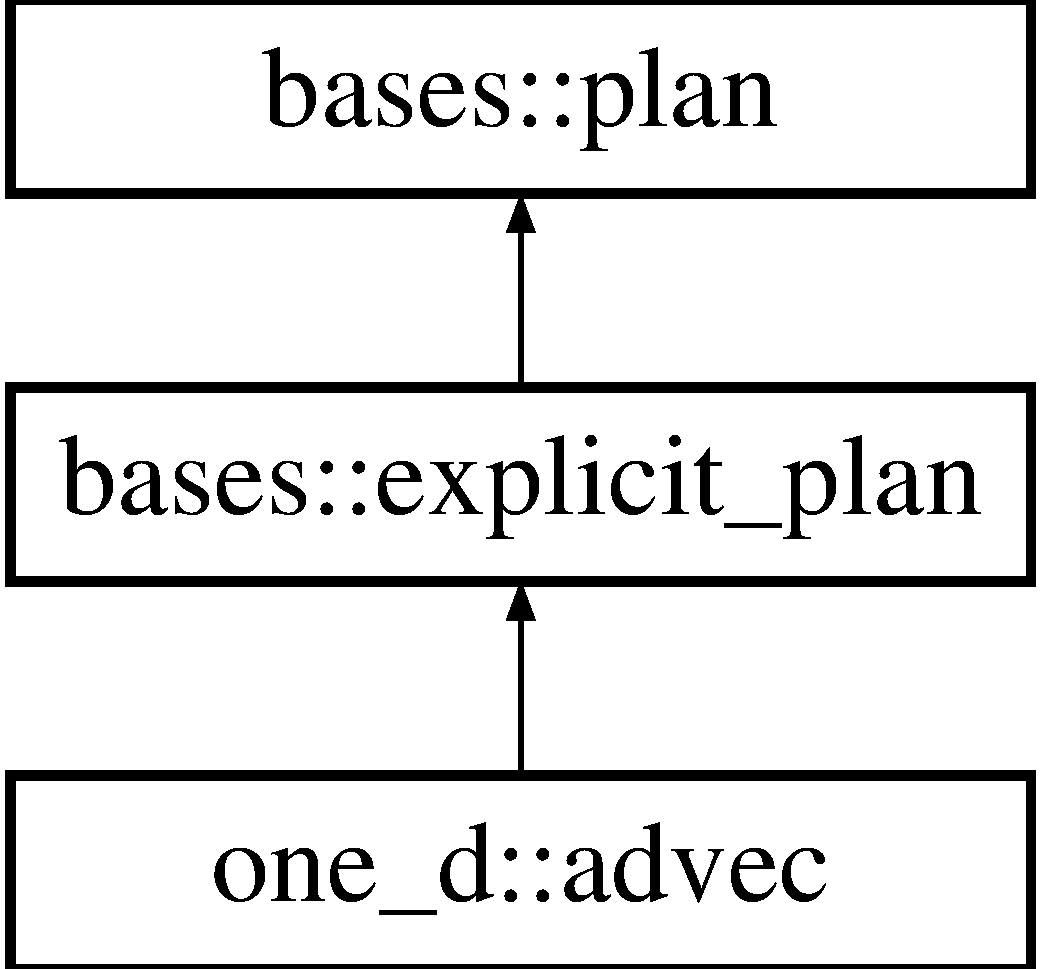
\includegraphics[height=3.000000cm]{classone__d_1_1advec}
\end{center}
\end{figure}
\subsection*{Public Member Functions}
\begin{DoxyCompactItemize}
\item 
\hypertarget{classone__d_1_1advec_a15229b440611b1f03ec254fa4c54d612}{{\bfseries advec} (\hyperlink{classbases_1_1element}{bases\-::element} $\ast$i\-\_\-element\-\_\-ptr, int i\-\_\-n, double i\-\_\-c, int i\-\_\-name\-\_\-in, int i\-\_\-name\-\_\-out, std\-::shared\-\_\-ptr$<$ \hyperlink{classbases_1_1collocation__grid}{bases\-::collocation\-\_\-grid} $>$ i\-\_\-grid)}\label{classone__d_1_1advec_a15229b440611b1f03ec254fa4c54d612}

\item 
void \hyperlink{classone__d_1_1advec_a1811538aec2a23cc27ef87fbce5dec8c}{execute} ()
\begin{DoxyCompactList}\small\item\em Operate the plan on the data arrays contained in the class. \end{DoxyCompactList}\end{DoxyCompactItemize}
\subsection*{Additional Inherited Members}


\subsection{Member Function Documentation}
\hypertarget{classone__d_1_1advec_a1811538aec2a23cc27ef87fbce5dec8c}{\index{one\-\_\-d\-::advec@{one\-\_\-d\-::advec}!execute@{execute}}
\index{execute@{execute}!one_d::advec@{one\-\_\-d\-::advec}}
\subsubsection[{execute}]{\setlength{\rightskip}{0pt plus 5cm}void one\-\_\-d\-::advec\-::execute (
\begin{DoxyParamCaption}
{}
\end{DoxyParamCaption}
)\hspace{0.3cm}{\ttfamily [virtual]}}}\label{classone__d_1_1advec_a1811538aec2a23cc27ef87fbce5dec8c}


Operate the plan on the data arrays contained in the class. 



 

 The plan class serves as a wrapper for this function. 

Reimplemented from \hyperlink{classbases_1_1explicit__plan_a21bcba4d429590031bba41ee2a48a4ef}{bases\-::explicit\-\_\-plan}.



The documentation for this class was generated from the following files\-:\begin{DoxyCompactItemize}
\item 
/\-Users/justinbrown/\-Dropbox/spectral\-\_\-element/src/one\-\_\-d/advection\-\_\-one\-\_\-d.\-h\item 
/\-Users/justinbrown/\-Dropbox/spectral\-\_\-element/src/one\-\_\-d/advection\-\_\-one\-\_\-d.\-cpp\end{DoxyCompactItemize}

\hypertarget{classone__d_1_1chebyshev_1_1advection__diffusion__element}{\section{one\-\_\-d\-:\-:chebyshev\-:\-:advection\-\_\-diffusion\-\_\-element Class Reference}
\label{classone__d_1_1chebyshev_1_1advection__diffusion__element}\index{one\-\_\-d\-::chebyshev\-::advection\-\_\-diffusion\-\_\-element@{one\-\_\-d\-::chebyshev\-::advection\-\_\-diffusion\-\_\-element}}
}


A simple implementation of the element class with diffusion.  




{\ttfamily \#include $<$element\-\_\-one\-\_\-d.\-hpp$>$}

Inheritance diagram for one\-\_\-d\-:\-:chebyshev\-:\-:advection\-\_\-diffusion\-\_\-element\-:\begin{figure}[H]
\begin{center}
\leavevmode
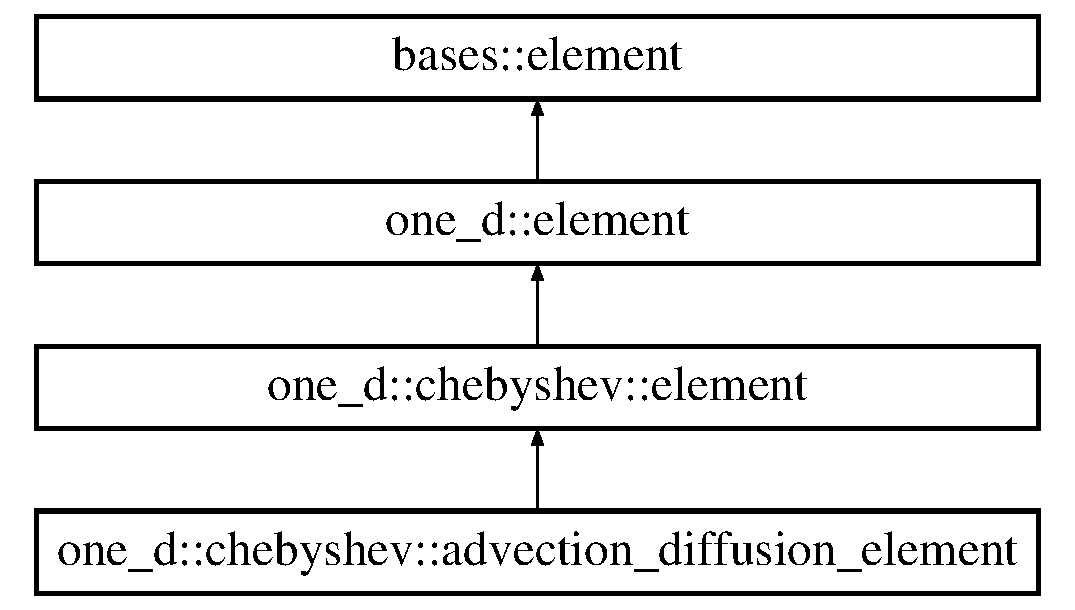
\includegraphics[height=4.000000cm]{classone__d_1_1chebyshev_1_1advection__diffusion__element}
\end{center}
\end{figure}
\subsection*{Public Member Functions}
\begin{DoxyCompactItemize}
\item 
\hyperlink{classone__d_1_1chebyshev_1_1advection__diffusion__element_aab3b41c17eb8806d8040ba75b03ed613}{advection\-\_\-diffusion\-\_\-element} (int i\-\_\-n, double i\-\_\-position\-\_\-0, double i\-\_\-position\-\_\-n, int i\-\_\-excess\-\_\-0, int i\-\_\-excess\-\_\-n, int i\-\_\-name, \hyperlink{namespaceio_a1c55c654666eeece6a9724f453fdbd87}{io\-::parameter\-\_\-map} \&i\-\_\-input\-Params, \hyperlink{classbases_1_1messenger}{bases\-::messenger} $\ast$i\-\_\-messenger\-\_\-ptr, int i\-\_\-flags)
\begin{DoxyCompactList}\small\item\em \end{DoxyCompactList}\item 
void \hyperlink{classone__d_1_1chebyshev_1_1advection__diffusion__element_a9f38631c75ee45cda5ce33ee51bddfc8}{implicit\-\_\-reset} ()
\begin{DoxyCompactList}\small\item\em Reset any matrices if necessary. \end{DoxyCompactList}\item 
virtual double \hyperlink{classone__d_1_1chebyshev_1_1advection__diffusion__element_a935392ea158d867bcc28733c72e3c9ae}{calculate\-\_\-timestep} ()
\begin{DoxyCompactList}\small\item\em Calculate the new timestep duration. \end{DoxyCompactList}\end{DoxyCompactItemize}
\subsection*{Additional Inherited Members}


\subsection{Detailed Description}
A simple implementation of the element class with diffusion. 



 This class contains a full element's capacity to run a single element diffusion in 1\-D with constant timestep. 

\subsection{Constructor \& Destructor Documentation}
\hypertarget{classone__d_1_1chebyshev_1_1advection__diffusion__element_aab3b41c17eb8806d8040ba75b03ed613}{\index{one\-\_\-d\-::chebyshev\-::advection\-\_\-diffusion\-\_\-element@{one\-\_\-d\-::chebyshev\-::advection\-\_\-diffusion\-\_\-element}!advection\-\_\-diffusion\-\_\-element@{advection\-\_\-diffusion\-\_\-element}}
\index{advection\-\_\-diffusion\-\_\-element@{advection\-\_\-diffusion\-\_\-element}!one_d::chebyshev::advection_diffusion_element@{one\-\_\-d\-::chebyshev\-::advection\-\_\-diffusion\-\_\-element}}
\subsubsection[{advection\-\_\-diffusion\-\_\-element}]{\setlength{\rightskip}{0pt plus 5cm}one\-\_\-d\-::chebyshev\-::advection\-\_\-diffusion\-\_\-element\-::advection\-\_\-diffusion\-\_\-element (
\begin{DoxyParamCaption}
\item[{int}]{i\-\_\-n, }
\item[{double}]{i\-\_\-position\-\_\-0, }
\item[{double}]{i\-\_\-position\-\_\-n, }
\item[{int}]{i\-\_\-excess\-\_\-0, }
\item[{int}]{i\-\_\-excess\-\_\-n, }
\item[{int}]{i\-\_\-name, }
\item[{{\bf io\-::parameter\-\_\-map} \&}]{i\-\_\-input\-Params, }
\item[{{\bf bases\-::messenger} $\ast$}]{i\-\_\-messenger\-\_\-ptr, }
\item[{int}]{i\-\_\-flags}
\end{DoxyParamCaption}
)}}\label{classone__d_1_1chebyshev_1_1advection__diffusion__element_aab3b41c17eb8806d8040ba75b03ed613}






 
\begin{DoxyParams}{Parameters}
{\em i\-\_\-excess\-\_\-0} & The integer number of points evaluated in the adjacent element \\
\hline
{\em i\-\_\-excess\-\_\-n} & The integer number of points evaluated in the adjacent element \\
\hline
\end{DoxyParams}


 

 
\begin{DoxyParams}{Parameters}
{\em i\-\_\-n} & The number of data elements in each scalar \\
\hline
{\em i\-\_\-position\-\_\-0} & The double position of index excess\-\_\-0 \\
\hline
{\em i\-\_\-position\-\_\-n} & The double position of index n -\/ 1 -\/ excess\-\_\-n \\
\hline
\end{DoxyParams}


 
\begin{DoxyParams}{Parameters}
{\em i\-\_\-name} & The string representation of the element \\
\hline
{\em n\-\_\-boundaries} & The integer number of boundaries (must be a multiple of 2) \\
\hline
{\em i\-\_\-input\-Params} & The parameter object that contains the input parameters of the run \\
\hline
{\em i\-\_\-messenger\-\_\-ptr} & A pointer to a messenger object \\
\hline
{\em i\-\_\-flags} & An integer set of execution flags \\
\hline
\end{DoxyParams}


\subsection{Member Function Documentation}
\hypertarget{classone__d_1_1chebyshev_1_1advection__diffusion__element_a935392ea158d867bcc28733c72e3c9ae}{\index{one\-\_\-d\-::chebyshev\-::advection\-\_\-diffusion\-\_\-element@{one\-\_\-d\-::chebyshev\-::advection\-\_\-diffusion\-\_\-element}!calculate\-\_\-timestep@{calculate\-\_\-timestep}}
\index{calculate\-\_\-timestep@{calculate\-\_\-timestep}!one_d::chebyshev::advection_diffusion_element@{one\-\_\-d\-::chebyshev\-::advection\-\_\-diffusion\-\_\-element}}
\subsubsection[{calculate\-\_\-timestep}]{\setlength{\rightskip}{0pt plus 5cm}double one\-\_\-d\-::chebyshev\-::advection\-\_\-diffusion\-\_\-element\-::calculate\-\_\-timestep (
\begin{DoxyParamCaption}
{}
\end{DoxyParamCaption}
)\hspace{0.3cm}{\ttfamily [virtual]}}}\label{classone__d_1_1chebyshev_1_1advection__diffusion__element_a935392ea158d867bcc28733c72e3c9ae}


Calculate the new timestep duration. 



 This method should be overwritten in the final class. It uses the knowledge of the user to beat numerical instabilities.

\begin{DoxyReturn}{Returns}
The double recommended timestep for the next timestep 
\end{DoxyReturn}


Implements \hyperlink{classbases_1_1element_aa8a344e596bf8cee3fdeda611b98bb1c}{bases\-::element}.

\hypertarget{classone__d_1_1chebyshev_1_1advection__diffusion__element_a9f38631c75ee45cda5ce33ee51bddfc8}{\index{one\-\_\-d\-::chebyshev\-::advection\-\_\-diffusion\-\_\-element@{one\-\_\-d\-::chebyshev\-::advection\-\_\-diffusion\-\_\-element}!implicit\-\_\-reset@{implicit\-\_\-reset}}
\index{implicit\-\_\-reset@{implicit\-\_\-reset}!one_d::chebyshev::advection_diffusion_element@{one\-\_\-d\-::chebyshev\-::advection\-\_\-diffusion\-\_\-element}}
\subsubsection[{implicit\-\_\-reset}]{\setlength{\rightskip}{0pt plus 5cm}void one\-\_\-d\-::chebyshev\-::advection\-\_\-diffusion\-\_\-element\-::implicit\-\_\-reset (
\begin{DoxyParamCaption}
{}
\end{DoxyParamCaption}
)\hspace{0.3cm}{\ttfamily [inline]}, {\ttfamily [virtual]}}}\label{classone__d_1_1chebyshev_1_1advection__diffusion__element_a9f38631c75ee45cda5ce33ee51bddfc8}


Reset any matrices if necessary. 



 

 This method should be overwritten if the element solves with an implicit part. It should only be called if the timestep duration has changed, for the most part. 

Reimplemented from \hyperlink{classbases_1_1element_a0311b32b397accaba0b9066c6c402274}{bases\-::element}.



The documentation for this class was generated from the following files\-:\begin{DoxyCompactItemize}
\item 
/\-Users/justinbrown/\-Dropbox/spectral\-\_\-element/src/one\-\_\-d/\hyperlink{element__one__d_8hpp}{element\-\_\-one\-\_\-d.\-hpp}\item 
/\-Users/justinbrown/\-Dropbox/spectral\-\_\-element/src/one\-\_\-d/\hyperlink{element__one__d_8cpp}{element\-\_\-one\-\_\-d.\-cpp}\end{DoxyCompactItemize}

\hypertarget{classchebyshev__grid}{\section{chebyshev\-\_\-grid Class Reference}
\label{classchebyshev__grid}\index{chebyshev\-\_\-grid@{chebyshev\-\_\-grid}}
}


A collocation grid for Chebyshev polynomials.  




{\ttfamily \#include $<$chebyshev.\-hpp$>$}

Inheritance diagram for chebyshev\-\_\-grid\-:\begin{figure}[H]
\begin{center}
\leavevmode
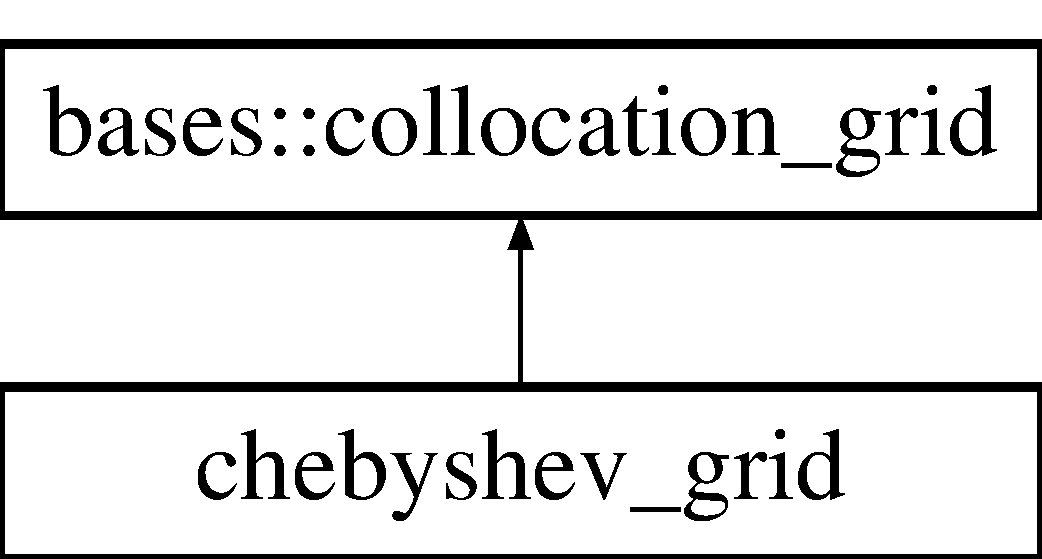
\includegraphics[height=2.000000cm]{classchebyshev__grid}
\end{center}
\end{figure}
\subsection*{Public Member Functions}
\begin{DoxyCompactItemize}
\item 
\hyperlink{classchebyshev__grid_ae37600b568e7d1e864b5ec10e6775c2d}{chebyshev\-\_\-grid} (int i\-\_\-\-M, int i\-\_\-\-N, double i\-\_\-scale=1.\-0, double i\-\_\-width=2.\-0)
\end{DoxyCompactItemize}
\subsection*{Additional Inherited Members}


\subsection{Detailed Description}
A collocation grid for Chebyshev polynomials. 



 This collocation grid stores the N collocation points for up to the Mth order Chebyshev polynomial and its first and second derivatives 

\subsection{Constructor \& Destructor Documentation}
\hypertarget{classchebyshev__grid_ae37600b568e7d1e864b5ec10e6775c2d}{\index{chebyshev\-\_\-grid@{chebyshev\-\_\-grid}!chebyshev\-\_\-grid@{chebyshev\-\_\-grid}}
\index{chebyshev\-\_\-grid@{chebyshev\-\_\-grid}!chebyshev_grid@{chebyshev\-\_\-grid}}
\subsubsection[{chebyshev\-\_\-grid}]{\setlength{\rightskip}{0pt plus 5cm}chebyshev\-\_\-grid\-::chebyshev\-\_\-grid (
\begin{DoxyParamCaption}
\item[{int}]{i\-\_\-\-M, }
\item[{int}]{i\-\_\-\-N, }
\item[{double}]{i\-\_\-scale = {\ttfamily 1.0}, }
\item[{double}]{i\-\_\-width = {\ttfamily 2.0}}
\end{DoxyParamCaption}
)}}\label{classchebyshev__grid_ae37600b568e7d1e864b5ec10e6775c2d}


 
\begin{DoxyParams}{Parameters}
{\em i\-\_\-\-M} & The integer max order of Chebyshev polynomial \\
\hline
{\em i\-\_\-\-N} & The integer number of collocation points \\
\hline
{\em i\-\_\-scale} & A double by which the grid should be scaled \\
\hline
{\em i\-\_\-width} & The double width of the collocation region \\
\hline
\end{DoxyParams}


The documentation for this class was generated from the following files\-:\begin{DoxyCompactItemize}
\item 
/\-Users/justinbrown/\-Dropbox/spectral\-\_\-element/src/utils/\hyperlink{chebyshev_8hpp}{chebyshev.\-hpp}\item 
/\-Users/justinbrown/\-Dropbox/spectral\-\_\-element/src/utils/\hyperlink{chebyshev_8cpp}{chebyshev.\-cpp}\end{DoxyCompactItemize}

\hypertarget{classbases_1_1collocation__grid}{\section{bases\-:\-:collocation\-\_\-grid Class Reference}
\label{classbases_1_1collocation__grid}\index{bases\-::collocation\-\_\-grid@{bases\-::collocation\-\_\-grid}}
}


A class containing a collocation grid.  




{\ttfamily \#include $<$collocation.\-hpp$>$}

Inheritance diagram for bases\-:\-:collocation\-\_\-grid\-:\begin{figure}[H]
\begin{center}
\leavevmode
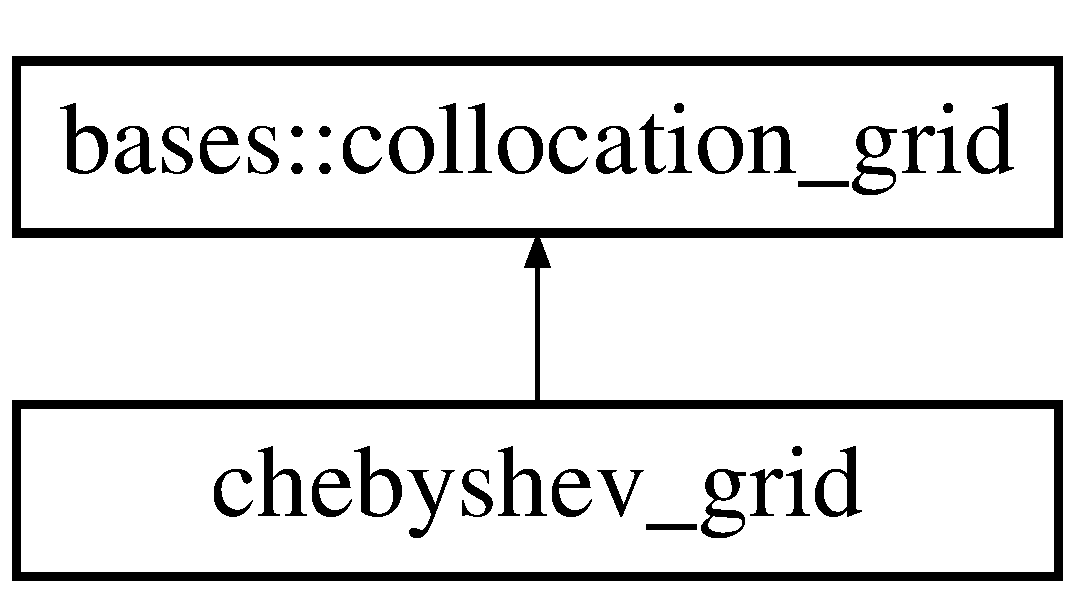
\includegraphics[height=2.000000cm]{classbases_1_1collocation__grid}
\end{center}
\end{figure}
\subsection*{Public Member Functions}
\begin{DoxyCompactItemize}
\item 
\hyperlink{classbases_1_1collocation__grid_a1413d667a9604794f460c5fd510d0cd4}{collocation\-\_\-grid} (int i\-\_\-derivs, int i\-\_\-rows, int i\-\_\-cols)
\item 
double \& \hyperlink{classbases_1_1collocation__grid_a61c927792d21388e43d077158b941de9}{index} (int deriv, int row, int col)
\begin{DoxyCompactList}\small\item\em An indexing operation into the grid, for convenience. \end{DoxyCompactList}\item 
double $\ast$ \hyperlink{classbases_1_1collocation__grid_a79757d7c1c12eacdbecf4c48ae67ef11}{get\-\_\-data} (int deriv)
\begin{DoxyCompactList}\small\item\em Get the data array for a given derivative level. \end{DoxyCompactList}\end{DoxyCompactItemize}
\subsection*{Protected Attributes}
\begin{DoxyCompactItemize}
\item 
\hypertarget{classbases_1_1collocation__grid_adcf647eb455d150b3c7c4c34bb33b1ae}{int \hyperlink{classbases_1_1collocation__grid_adcf647eb455d150b3c7c4c34bb33b1ae}{rows}}\label{classbases_1_1collocation__grid_adcf647eb455d150b3c7c4c34bb33b1ae}

\begin{DoxyCompactList}\small\item\em The integer number of rows in the grid. \end{DoxyCompactList}\item 
\hypertarget{classbases_1_1collocation__grid_ac42def515322bb14f572ef564d7101d8}{int \hyperlink{classbases_1_1collocation__grid_ac42def515322bb14f572ef564d7101d8}{cols}}\label{classbases_1_1collocation__grid_ac42def515322bb14f572ef564d7101d8}

\begin{DoxyCompactList}\small\item\em The integer number of columns in the grid. \end{DoxyCompactList}\item 
\hypertarget{classbases_1_1collocation__grid_a696572e39da7ee8ab64f3300db8b0408}{int \hyperlink{classbases_1_1collocation__grid_a696572e39da7ee8ab64f3300db8b0408}{derivs}}\label{classbases_1_1collocation__grid_a696572e39da7ee8ab64f3300db8b0408}

\begin{DoxyCompactList}\small\item\em The integer number of derivatives deep the collocation grid runs. \end{DoxyCompactList}\end{DoxyCompactItemize}


\subsection{Detailed Description}
A class containing a collocation grid. 



 This will need to be instantiated for a collocation method. Ideally, the structure contains a grid of polynomial values at a number of collocation points which can be called for little temporal expense. 

\subsection{Constructor \& Destructor Documentation}
\hypertarget{classbases_1_1collocation__grid_a1413d667a9604794f460c5fd510d0cd4}{\index{bases\-::collocation\-\_\-grid@{bases\-::collocation\-\_\-grid}!collocation\-\_\-grid@{collocation\-\_\-grid}}
\index{collocation\-\_\-grid@{collocation\-\_\-grid}!bases::collocation_grid@{bases\-::collocation\-\_\-grid}}
\subsubsection[{collocation\-\_\-grid}]{\setlength{\rightskip}{0pt plus 5cm}bases\-::collocation\-\_\-grid\-::collocation\-\_\-grid (
\begin{DoxyParamCaption}
\item[{int}]{i\-\_\-derivs, }
\item[{int}]{i\-\_\-rows, }
\item[{int}]{i\-\_\-cols}
\end{DoxyParamCaption}
)}}\label{classbases_1_1collocation__grid_a1413d667a9604794f460c5fd510d0cd4}


 
\begin{DoxyParams}{Parameters}
{\em i\-\_\-derivs} & The integer number of derivatives in the grid \\
\hline
{\em i\-\_\-rows} & The integer number of rows in the grid \\
\hline
{\em i\-\_\-cols} & The integer number of columns in the grid \\
\hline
\end{DoxyParams}


\subsection{Member Function Documentation}
\hypertarget{classbases_1_1collocation__grid_a79757d7c1c12eacdbecf4c48ae67ef11}{\index{bases\-::collocation\-\_\-grid@{bases\-::collocation\-\_\-grid}!get\-\_\-data@{get\-\_\-data}}
\index{get\-\_\-data@{get\-\_\-data}!bases::collocation_grid@{bases\-::collocation\-\_\-grid}}
\subsubsection[{get\-\_\-data}]{\setlength{\rightskip}{0pt plus 5cm}double$\ast$ bases\-::collocation\-\_\-grid\-::get\-\_\-data (
\begin{DoxyParamCaption}
\item[{int}]{deriv}
\end{DoxyParamCaption}
)\hspace{0.3cm}{\ttfamily [inline]}}}\label{classbases_1_1collocation__grid_a79757d7c1c12eacdbecf4c48ae67ef11}


Get the data array for a given derivative level. 



 This method is intended for use when a subroutine requires the matrix containing the collocation elements.


\begin{DoxyParams}{Parameters}
{\em deriv} & An integer derivative level (0 = value, 1 = first derivative, ...)\\
\hline
\end{DoxyParams}
\begin{DoxyReturn}{Returns}
A pointer to the first element of the double data array 
\end{DoxyReturn}
\hypertarget{classbases_1_1collocation__grid_a61c927792d21388e43d077158b941de9}{\index{bases\-::collocation\-\_\-grid@{bases\-::collocation\-\_\-grid}!index@{index}}
\index{index@{index}!bases::collocation_grid@{bases\-::collocation\-\_\-grid}}
\subsubsection[{index}]{\setlength{\rightskip}{0pt plus 5cm}double\& bases\-::collocation\-\_\-grid\-::index (
\begin{DoxyParamCaption}
\item[{int}]{deriv, }
\item[{int}]{row, }
\item[{int}]{col}
\end{DoxyParamCaption}
)\hspace{0.3cm}{\ttfamily [inline]}}}\label{classbases_1_1collocation__grid_a61c927792d21388e43d077158b941de9}


An indexing operation into the grid, for convenience. 



 
\begin{DoxyParams}{Parameters}
{\em deriv} & The integer deriv to be indexed \\
\hline
{\em row} & The integer row to be indexed \\
\hline
{\em col} & The integer column to be indexed\\
\hline
\end{DoxyParams}
\begin{DoxyReturn}{Returns}
The double value at the index 
\end{DoxyReturn}


The documentation for this class was generated from the following files\-:\begin{DoxyCompactItemize}
\item 
/\-Users/justinbrown/\-Dropbox/spectral\-\_\-element/src/bases/\hyperlink{collocation_8hpp}{collocation.\-hpp}\item 
/\-Users/justinbrown/\-Dropbox/spectral\-\_\-element/src/bases/\hyperlink{collocation_8cpp}{collocation.\-cpp}\end{DoxyCompactItemize}

\hypertarget{classone__d_1_1chebyshev_1_1cuda__element}{\section{one\-\_\-d\-:\-:chebyshev\-:\-:cuda\-\_\-element Class Reference}
\label{classone__d_1_1chebyshev_1_1cuda__element}\index{one\-\_\-d\-::chebyshev\-::cuda\-\_\-element@{one\-\_\-d\-::chebyshev\-::cuda\-\_\-element}}
}
Inheritance diagram for one\-\_\-d\-:\-:chebyshev\-:\-:cuda\-\_\-element\-:\begin{figure}[H]
\begin{center}
\leavevmode
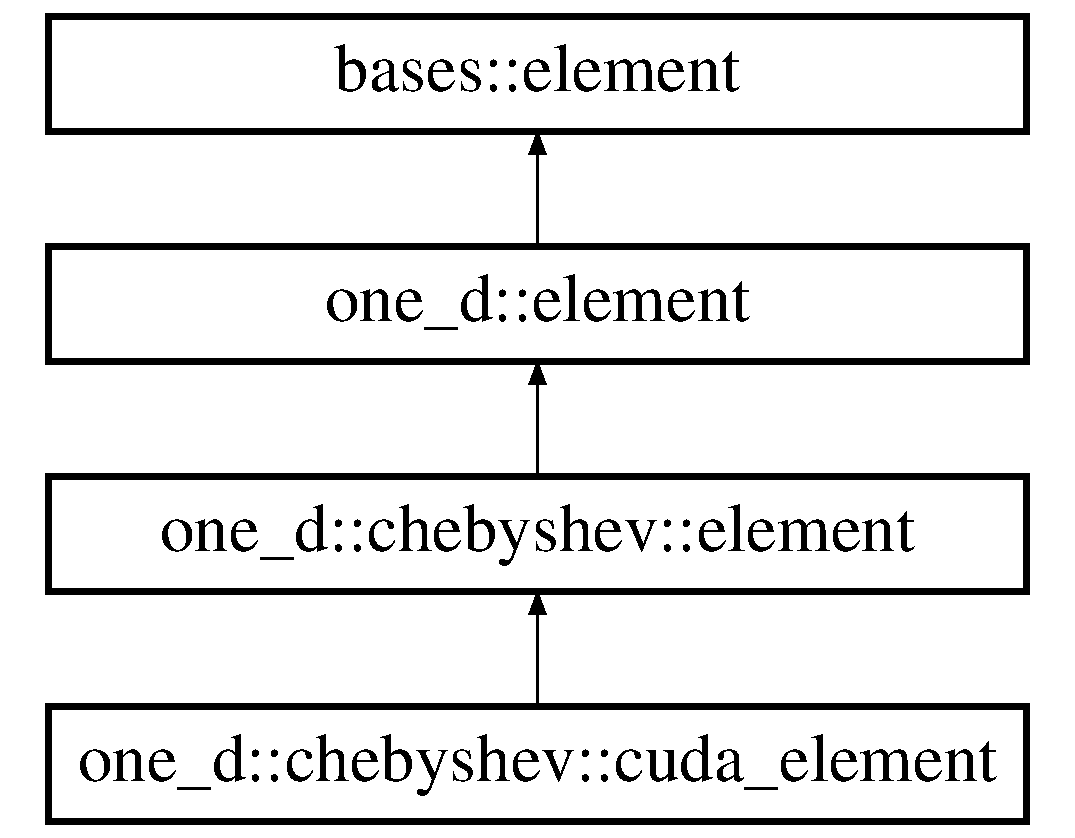
\includegraphics[height=4.000000cm]{classone__d_1_1chebyshev_1_1cuda__element}
\end{center}
\end{figure}
\subsection*{Public Member Functions}
\begin{DoxyCompactItemize}
\item 
\hypertarget{classone__d_1_1chebyshev_1_1cuda__element_a2a501d087aa0072a5feb79a594b108a3}{{\bfseries cuda\-\_\-element} (int i\-\_\-n, double i\-\_\-position\-\_\-0, double i\-\_\-position\-\_\-n, int i\-\_\-excess\-\_\-0, int i\-\_\-excess\-\_\-n, int i\-\_\-name, \hyperlink{namespaceio_a1c55c654666eeece6a9724f453fdbd87}{io\-::parameter\-\_\-map} \&i\-\_\-input\-\_\-\-Params, \hyperlink{classbases_1_1messenger}{bases\-::messenger} $\ast$i\-\_\-messenger\-\_\-ptr, int i\-\_\-flags)}\label{classone__d_1_1chebyshev_1_1cuda__element_a2a501d087aa0072a5feb79a594b108a3}

\item 
void \hyperlink{classone__d_1_1chebyshev_1_1cuda__element_ac304ac234f63b576d3acab5c31c9a31f}{implicit\-\_\-reset} ()
\begin{DoxyCompactList}\small\item\em Reset any matrices if necessary. \end{DoxyCompactList}\item 
virtual double \hyperlink{classone__d_1_1chebyshev_1_1cuda__element_a528350be3f4edf1470ca31576b3f7ea2}{calculate\-\_\-timestep} ()
\begin{DoxyCompactList}\small\item\em Calculate the new timestep duration. \end{DoxyCompactList}\end{DoxyCompactItemize}
\subsection*{Additional Inherited Members}


\subsection{Member Function Documentation}
\hypertarget{classone__d_1_1chebyshev_1_1cuda__element_a528350be3f4edf1470ca31576b3f7ea2}{\index{one\-\_\-d\-::chebyshev\-::cuda\-\_\-element@{one\-\_\-d\-::chebyshev\-::cuda\-\_\-element}!calculate\-\_\-timestep@{calculate\-\_\-timestep}}
\index{calculate\-\_\-timestep@{calculate\-\_\-timestep}!one_d::chebyshev::cuda_element@{one\-\_\-d\-::chebyshev\-::cuda\-\_\-element}}
\subsubsection[{calculate\-\_\-timestep}]{\setlength{\rightskip}{0pt plus 5cm}double one\-\_\-d\-::chebyshev\-::cuda\-\_\-element\-::calculate\-\_\-timestep (
\begin{DoxyParamCaption}
{}
\end{DoxyParamCaption}
)\hspace{0.3cm}{\ttfamily [virtual]}}}\label{classone__d_1_1chebyshev_1_1cuda__element_a528350be3f4edf1470ca31576b3f7ea2}


Calculate the new timestep duration. 



 This method should be overwritten in the final class. It uses the knowledge of the user to beat numerical instabilities.

\begin{DoxyReturn}{Returns}
The double recommended timestep for the next timestep 
\end{DoxyReturn}


Implements \hyperlink{classbases_1_1element_aa8a344e596bf8cee3fdeda611b98bb1c}{bases\-::element}.

\hypertarget{classone__d_1_1chebyshev_1_1cuda__element_ac304ac234f63b576d3acab5c31c9a31f}{\index{one\-\_\-d\-::chebyshev\-::cuda\-\_\-element@{one\-\_\-d\-::chebyshev\-::cuda\-\_\-element}!implicit\-\_\-reset@{implicit\-\_\-reset}}
\index{implicit\-\_\-reset@{implicit\-\_\-reset}!one_d::chebyshev::cuda_element@{one\-\_\-d\-::chebyshev\-::cuda\-\_\-element}}
\subsubsection[{implicit\-\_\-reset}]{\setlength{\rightskip}{0pt plus 5cm}void one\-\_\-d\-::chebyshev\-::cuda\-\_\-element\-::implicit\-\_\-reset (
\begin{DoxyParamCaption}
{}
\end{DoxyParamCaption}
)\hspace{0.3cm}{\ttfamily [inline]}, {\ttfamily [virtual]}}}\label{classone__d_1_1chebyshev_1_1cuda__element_ac304ac234f63b576d3acab5c31c9a31f}


Reset any matrices if necessary. 



 This method should be overwritten if the element solves with an implicit part. It should only be called if the timestep duration has changed, for the most part. 

Reimplemented from \hyperlink{classbases_1_1element_a0311b32b397accaba0b9066c6c402274}{bases\-::element}.



The documentation for this class was generated from the following files\-:\begin{DoxyCompactItemize}
\item 
/\-Users/justinbrown/\-Dropbox/spectral\-\_\-element/src/one\-\_\-d/\hyperlink{element__one__d_8hpp}{element\-\_\-one\-\_\-d.\-hpp}\item 
/\-Users/justinbrown/\-Dropbox/spectral\-\_\-element/src/one\-\_\-d/\hyperlink{element__one__d_8cpp}{element\-\_\-one\-\_\-d.\-cpp}\end{DoxyCompactItemize}

\hypertarget{classbases_1_1element}{\section{bases\-:\-:element Class Reference}
\label{classbases_1_1element}\index{bases\-::element@{bases\-::element}}
}


This is the basic class of the code.  




{\ttfamily \#include $<$element.\-hpp$>$}

Inheritance diagram for bases\-:\-:element\-:\begin{figure}[H]
\begin{center}
\leavevmode
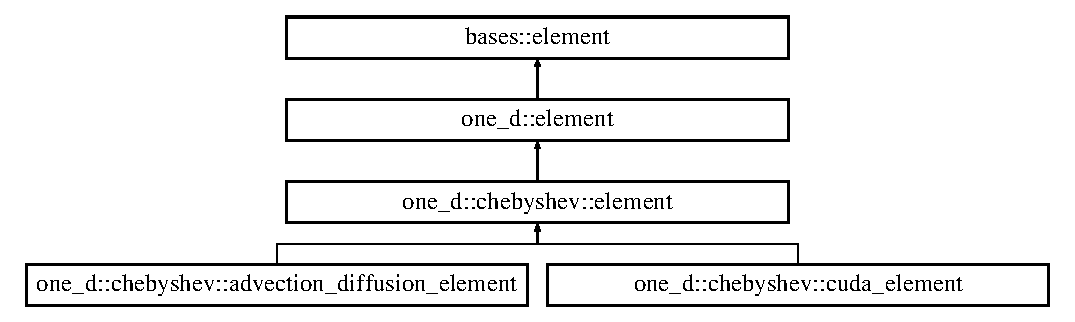
\includegraphics[height=3.875432cm]{classbases_1_1element}
\end{center}
\end{figure}
\subsection*{Public Types}
\begin{DoxyCompactItemize}
\item 
typedef std\-::vector$<$ int $>$\\*
\-::\hyperlink{classbases_1_1element_ad6c297b8fbb3ea61a1a7048f0fbf7d89}{iterator} \hyperlink{classbases_1_1element_ad6c297b8fbb3ea61a1a7048f0fbf7d89}{iterator}
\begin{DoxyCompactList}\small\item\em An iterator for the element class. \end{DoxyCompactList}\end{DoxyCompactItemize}
\subsection*{Public Member Functions}
\begin{DoxyCompactItemize}
\item 
\hyperlink{classbases_1_1element_a06505a1d8050683b6a9a07b4b92f38f5}{element} (int i\-\_\-name, int n\-\_\-boundaries, \hyperlink{namespaceio_a1c55c654666eeece6a9724f453fdbd87}{io\-::parameter\-\_\-map} \&i\-\_\-input\-Params, \hyperlink{classbases_1_1messenger}{messenger} $\ast$i\-\_\-messenger\-\_\-ptr, int i\-\_\-flags)
\item 
virtual double \& \hyperlink{classbases_1_1element_a4ae6c42893603fc086c5c207e236f9d8}{operator\mbox{[}$\,$\mbox{]}} (int \hyperlink{classbases_1_1element_a52af85c34174ec732a3feb6a7e63fbc6}{name})=0
\begin{DoxyCompactList}\small\item\em Get the double reference to the named scalar. \end{DoxyCompactList}\item 
virtual double \& \hyperlink{classbases_1_1element_aec8a0151fcc9259e3313558a928fdf62}{operator()} (int \hyperlink{classbases_1_1element_a52af85c34174ec732a3feb6a7e63fbc6}{name}, int \hyperlink{plan_8hpp_a6784e1c334dfceb8f017667c0b0f6a3e}{index}=0)
\begin{DoxyCompactList}\small\item\em Get the double reference to the given index of the named scalar. \end{DoxyCompactList}\item 
virtual \hyperlink{classbases_1_1element_ad6c297b8fbb3ea61a1a7048f0fbf7d89}{iterator} \hyperlink{classbases_1_1element_aa323f71efe1d063f3a75fb0ae52dd4e4}{begin} ()
\begin{DoxyCompactList}\small\item\em Get the iterator for the class at the first scalar index. \end{DoxyCompactList}\item 
virtual \hyperlink{classbases_1_1element_ad6c297b8fbb3ea61a1a7048f0fbf7d89}{iterator} \hyperlink{classbases_1_1element_a56ecd5c3a4ca85b1a818c9ff0d0d0213}{end} ()
\begin{DoxyCompactList}\small\item\em Get the iterator for the class at the last scalar index. \end{DoxyCompactList}\item 
void \hyperlink{classbases_1_1element_a4db7290cae3a85a32e28a6f73457c08c}{set\-\_\-grid} (std\-::shared\-\_\-ptr$<$ \hyperlink{classbases_1_1collocation__grid}{collocation\-\_\-grid} $>$ i\-\_\-grid)
\begin{DoxyCompactList}\small\item\em Set the collocation grid. \end{DoxyCompactList}\item 
void \hyperlink{classbases_1_1element_a798c23f47fb27d78569619cff8a03cf8}{add\-\_\-solver} (std\-::shared\-\_\-ptr$<$ \hyperlink{classbases_1_1solver}{solver} $>$ i\-\_\-solver)
\begin{DoxyCompactList}\small\item\em Set the matrix solver. \end{DoxyCompactList}\item 
void \hyperlink{classbases_1_1element_a9e46cf2492d82e9574ebcdbd39be3391}{add\-\_\-transform} (std\-::shared\-\_\-ptr$<$ \hyperlink{classbases_1_1plan}{plan} $>$ i\-\_\-plan)
\begin{DoxyCompactList}\small\item\em Set the transform operation. \end{DoxyCompactList}\item 
void \hyperlink{classbases_1_1element_aa3ee0ec9bda610aead7a6c8a02b84e19}{add\-\_\-pre\-\_\-plan} (std\-::shared\-\_\-ptr$<$ \hyperlink{classbases_1_1plan}{plan} $>$ i\-\_\-plan)
\begin{DoxyCompactList}\small\item\em Adds a plan to be executed in order. \end{DoxyCompactList}\item 
void \hyperlink{classbases_1_1element_aac0b4f2a8cf1aa6f6831ba99fe9d32df}{add\-\_\-post\-\_\-plan} (std\-::shared\-\_\-ptr$<$ \hyperlink{classbases_1_1plan}{plan} $>$ i\-\_\-plan)
\begin{DoxyCompactList}\small\item\em Adds a plan to be executed in order. \end{DoxyCompactList}\item 
void \hyperlink{classbases_1_1element_ad1ebcca153d00d0279df6c395ad91e83}{add\-\_\-implicit\-\_\-plan} (std\-::shared\-\_\-ptr$<$ \hyperlink{classbases_1_1plan}{plan} $>$ i\-\_\-plan)
\begin{DoxyCompactList}\small\item\em Adds an implicit plan to be executed in order once at the start. \end{DoxyCompactList}\item 
virtual void \hyperlink{classbases_1_1element_a8c0350a45f7aff09ba8ebbfb2a789027}{initialize} (int \hyperlink{classbases_1_1element_a52af85c34174ec732a3feb6a7e63fbc6}{name}, double $\ast$initial\-\_\-conditions=N\-U\-L\-L)=0
\begin{DoxyCompactList}\small\item\em Initialize the scalar name. \end{DoxyCompactList}\item 
virtual void \hyperlink{classbases_1_1element_ac2a829e5dc54ab249d8b567f608e7f69}{explicit\-\_\-reset} ()
\begin{DoxyCompactList}\small\item\em Reset every scalar index $<$ 0 and converts to spectral space. \end{DoxyCompactList}\item 
virtual void \hyperlink{classbases_1_1element_a0311b32b397accaba0b9066c6c402274}{implicit\-\_\-reset} ()
\begin{DoxyCompactList}\small\item\em Reset any matrices if necessary. \end{DoxyCompactList}\item 
virtual void \hyperlink{classbases_1_1element_aebdb8f7c290f78cc9e9abb019e96eeaf}{transform\-\_\-inverse} ()
\begin{DoxyCompactList}\small\item\em Transform from spectral space to physical space. \end{DoxyCompactList}\item 
\hypertarget{classbases_1_1element_acd5b77ded6283aec184192d313ee17e8}{virtual void {\bfseries solve} ()}\label{classbases_1_1element_acd5b77ded6283aec184192d313ee17e8}

\item 
virtual double \hyperlink{classbases_1_1element_aa8a344e596bf8cee3fdeda611b98bb1c}{calculate\-\_\-timestep} ()=0
\begin{DoxyCompactList}\small\item\em Calculate the new timestep duration. \end{DoxyCompactList}\item 
virtual void \hyperlink{classbases_1_1element_a86a15277a82abbc28ba75f67817e170a}{execute\-\_\-boundaries} ()=0
\begin{DoxyCompactList}\small\item\em Execute the boundary conditions. \end{DoxyCompactList}\item 
virtual void \hyperlink{classbases_1_1element_a4a8ef296f0853fc3e1941b696eee7dc9}{run} ()
\begin{DoxyCompactList}\small\item\em The main function call of the class. \end{DoxyCompactList}\item 
virtual void \hyperlink{classbases_1_1element_a8924e3a51b3c02433c082ebbb94c47d0}{failsafe} ()
\begin{DoxyCompactList}\small\item\em Output all information to a dump file in the current directory. \end{DoxyCompactList}\end{DoxyCompactItemize}
\subsection*{Protected Attributes}
\begin{DoxyCompactItemize}
\item 
\hypertarget{classbases_1_1element_a52af85c34174ec732a3feb6a7e63fbc6}{int \hyperlink{classbases_1_1element_a52af85c34174ec732a3feb6a7e63fbc6}{name}}\label{classbases_1_1element_a52af85c34174ec732a3feb6a7e63fbc6}

\begin{DoxyCompactList}\small\item\em An integer representation of the element, to be used in file output. \end{DoxyCompactList}\item 
\hypertarget{classbases_1_1element_adac9bb89cc00150c2546e9880e0f677a}{\hyperlink{namespaceio_a1c55c654666eeece6a9724f453fdbd87}{io\-::parameter\-\_\-map} \& \hyperlink{classbases_1_1element_adac9bb89cc00150c2546e9880e0f677a}{input\-Params}}\label{classbases_1_1element_adac9bb89cc00150c2546e9880e0f677a}

\begin{DoxyCompactList}\small\item\em The map that contains the input parameters. \end{DoxyCompactList}\item 
\hypertarget{classbases_1_1element_a0ca8319905d8702294384d940a5cf0f7}{\hyperlink{classbases_1_1messenger}{messenger} $\ast$ \hyperlink{classbases_1_1element_a0ca8319905d8702294384d940a5cf0f7}{messenger\-\_\-ptr}}\label{classbases_1_1element_a0ca8319905d8702294384d940a5cf0f7}

\begin{DoxyCompactList}\small\item\em A pointer to the messenger object. \end{DoxyCompactList}\item 
\hypertarget{classbases_1_1element_ae96e3c9a7a8c0aa53e6f98e62ecf23af}{int \hyperlink{classbases_1_1element_ae96e3c9a7a8c0aa53e6f98e62ecf23af}{flags}}\label{classbases_1_1element_ae96e3c9a7a8c0aa53e6f98e62ecf23af}

\begin{DoxyCompactList}\small\item\em An integer set of execution flags. \end{DoxyCompactList}\item 
\hypertarget{classbases_1_1element_a47315779623a1472300076f4df1c713b}{double \hyperlink{classbases_1_1element_a47315779623a1472300076f4df1c713b}{duration}}\label{classbases_1_1element_a47315779623a1472300076f4df1c713b}

\begin{DoxyCompactList}\small\item\em The double total simulated time. \end{DoxyCompactList}\item 
\hypertarget{classbases_1_1element_ac0bd283b49358bd1f5a0b6ec0e1daae0}{double \hyperlink{classbases_1_1element_ac0bd283b49358bd1f5a0b6ec0e1daae0}{timestep}}\label{classbases_1_1element_ac0bd283b49358bd1f5a0b6ec0e1daae0}

\begin{DoxyCompactList}\small\item\em The double timestep length. \end{DoxyCompactList}\item 
\hypertarget{classbases_1_1element_aa8c487033b765147186f5904cbfe39a6}{std\-::vector$<$ int $>$ \hyperlink{classbases_1_1element_aa8c487033b765147186f5904cbfe39a6}{names}}\label{classbases_1_1element_aa8c487033b765147186f5904cbfe39a6}

\begin{DoxyCompactList}\small\item\em A vector of integer name indices of the contained scalars. \end{DoxyCompactList}\item 
\hypertarget{classbases_1_1element_a0be44a6a3cef50bf30850759c9c1f433}{std\-::shared\-\_\-ptr$<$ \hyperlink{classbases_1_1collocation__grid}{collocation\-\_\-grid} $>$ \hyperlink{classbases_1_1element_a0be44a6a3cef50bf30850759c9c1f433}{grid}}\label{classbases_1_1element_a0be44a6a3cef50bf30850759c9c1f433}

\begin{DoxyCompactList}\small\item\em A shared pointer to the collocation grid. \end{DoxyCompactList}\item 
\hypertarget{classbases_1_1element_afe96a343a5fea6c7894a5a78bf460155}{std\-::shared\-\_\-ptr$<$ \hyperlink{classio_1_1output}{io\-::output} $>$ \hyperlink{classbases_1_1element_afe96a343a5fea6c7894a5a78bf460155}{failsafe\-\_\-dump}}\label{classbases_1_1element_afe96a343a5fea6c7894a5a78bf460155}

\begin{DoxyCompactList}\small\item\em An implementation to dump in case of failure. \end{DoxyCompactList}\item 
\hypertarget{classbases_1_1element_a876491b92ecc30b15971b72a04199262}{std\-::shared\-\_\-ptr$<$ \hyperlink{classio_1_1output}{io\-::output} $>$ \hyperlink{classbases_1_1element_a876491b92ecc30b15971b72a04199262}{normal\-\_\-stream}}\label{classbases_1_1element_a876491b92ecc30b15971b72a04199262}

\begin{DoxyCompactList}\small\item\em An implementation to output in normal space. \end{DoxyCompactList}\item 
\hypertarget{classbases_1_1element_a9f154ce2a7a6cb41810a412d56dc0d05}{std\-::shared\-\_\-ptr$<$ \hyperlink{classio_1_1output}{io\-::output} $>$ \hyperlink{classbases_1_1element_a9f154ce2a7a6cb41810a412d56dc0d05}{transform\-\_\-stream}}\label{classbases_1_1element_a9f154ce2a7a6cb41810a412d56dc0d05}

\begin{DoxyCompactList}\small\item\em An implementation to output in transform space. \end{DoxyCompactList}\item 
\hypertarget{classbases_1_1element_a4bfaed78e051894cdcb980272953a8df}{std\-::vector$<$ double $>$ \hyperlink{classbases_1_1element_a4bfaed78e051894cdcb980272953a8df}{boundary\-\_\-weights}}\label{classbases_1_1element_a4bfaed78e051894cdcb980272953a8df}

\begin{DoxyCompactList}\small\item\em A double vector of boundary weights. \end{DoxyCompactList}\end{DoxyCompactItemize}
\subsection*{Friends}
\begin{DoxyCompactItemize}
\item 
\hypertarget{classbases_1_1element_a09a337604df64eed6477718d9f120f91}{class {\bfseries plan}}\label{classbases_1_1element_a09a337604df64eed6477718d9f120f91}

\end{DoxyCompactItemize}


\subsection{Detailed Description}
This is the basic class of the code. 



 A true run will contain multiple elements linked together at the boundaries. This code is designed to work by the collocation method. 

\subsection{Member Typedef Documentation}
\hypertarget{classbases_1_1element_ad6c297b8fbb3ea61a1a7048f0fbf7d89}{\index{bases\-::element@{bases\-::element}!iterator@{iterator}}
\index{iterator@{iterator}!bases::element@{bases\-::element}}
\subsubsection[{iterator}]{\setlength{\rightskip}{0pt plus 5cm}typedef std\-::vector$<$int$>$\-::{\bf iterator} {\bf bases\-::element\-::iterator}}}\label{classbases_1_1element_ad6c297b8fbb3ea61a1a7048f0fbf7d89}


An iterator for the element class. 



 This iterator steps through the scalar fields in the order they were added. 

\subsection{Constructor \& Destructor Documentation}
\hypertarget{classbases_1_1element_a06505a1d8050683b6a9a07b4b92f38f5}{\index{bases\-::element@{bases\-::element}!element@{element}}
\index{element@{element}!bases::element@{bases\-::element}}
\subsubsection[{element}]{\setlength{\rightskip}{0pt plus 5cm}bases\-::element\-::element (
\begin{DoxyParamCaption}
\item[{int}]{i\-\_\-name, }
\item[{int}]{n\-\_\-boundaries, }
\item[{{\bf io\-::parameter\-\_\-map} \&}]{i\-\_\-input\-Params, }
\item[{{\bf messenger} $\ast$}]{i\-\_\-messenger\-\_\-ptr, }
\item[{int}]{i\-\_\-flags}
\end{DoxyParamCaption}
)\hspace{0.3cm}{\ttfamily [inline]}}}\label{classbases_1_1element_a06505a1d8050683b6a9a07b4b92f38f5}


 
\begin{DoxyParams}{Parameters}
{\em i\-\_\-name} & The string representation of the element \\
\hline
{\em n\-\_\-boundaries} & The integer number of boundaries (must be a multiple of 2) \\
\hline
{\em i\-\_\-input\-Params} & The parameter object that contains the input parameters of the run \\
\hline
{\em i\-\_\-messenger\-\_\-ptr} & A pointer to a messenger object \\
\hline
{\em i\-\_\-flags} & An integer set of execution flags \\
\hline
\end{DoxyParams}


\subsection{Member Function Documentation}
\hypertarget{classbases_1_1element_ad1ebcca153d00d0279df6c395ad91e83}{\index{bases\-::element@{bases\-::element}!add\-\_\-implicit\-\_\-plan@{add\-\_\-implicit\-\_\-plan}}
\index{add\-\_\-implicit\-\_\-plan@{add\-\_\-implicit\-\_\-plan}!bases::element@{bases\-::element}}
\subsubsection[{add\-\_\-implicit\-\_\-plan}]{\setlength{\rightskip}{0pt plus 5cm}void bases\-::element\-::add\-\_\-implicit\-\_\-plan (
\begin{DoxyParamCaption}
\item[{std\-::shared\-\_\-ptr$<$ {\bf plan} $>$}]{i\-\_\-plan}
\end{DoxyParamCaption}
)\hspace{0.3cm}{\ttfamily [inline]}}}\label{classbases_1_1element_ad1ebcca153d00d0279df6c395ad91e83}


Adds an implicit plan to be executed in order once at the start. 



 
\begin{DoxyParams}{Parameters}
{\em i\-\_\-plan} & A shared pointer to the plan to add \\
\hline
\end{DoxyParams}
\hypertarget{classbases_1_1element_aac0b4f2a8cf1aa6f6831ba99fe9d32df}{\index{bases\-::element@{bases\-::element}!add\-\_\-post\-\_\-plan@{add\-\_\-post\-\_\-plan}}
\index{add\-\_\-post\-\_\-plan@{add\-\_\-post\-\_\-plan}!bases::element@{bases\-::element}}
\subsubsection[{add\-\_\-post\-\_\-plan}]{\setlength{\rightskip}{0pt plus 5cm}void bases\-::element\-::add\-\_\-post\-\_\-plan (
\begin{DoxyParamCaption}
\item[{std\-::shared\-\_\-ptr$<$ {\bf plan} $>$}]{i\-\_\-plan}
\end{DoxyParamCaption}
)\hspace{0.3cm}{\ttfamily [inline]}}}\label{classbases_1_1element_aac0b4f2a8cf1aa6f6831ba99fe9d32df}


Adds a plan to be executed in order. 



 
\begin{DoxyParams}{Parameters}
{\em i\-\_\-plan} & A shared pointer to the plan to add \\
\hline
\end{DoxyParams}
\hypertarget{classbases_1_1element_aa3ee0ec9bda610aead7a6c8a02b84e19}{\index{bases\-::element@{bases\-::element}!add\-\_\-pre\-\_\-plan@{add\-\_\-pre\-\_\-plan}}
\index{add\-\_\-pre\-\_\-plan@{add\-\_\-pre\-\_\-plan}!bases::element@{bases\-::element}}
\subsubsection[{add\-\_\-pre\-\_\-plan}]{\setlength{\rightskip}{0pt plus 5cm}void bases\-::element\-::add\-\_\-pre\-\_\-plan (
\begin{DoxyParamCaption}
\item[{std\-::shared\-\_\-ptr$<$ {\bf plan} $>$}]{i\-\_\-plan}
\end{DoxyParamCaption}
)\hspace{0.3cm}{\ttfamily [inline]}}}\label{classbases_1_1element_aa3ee0ec9bda610aead7a6c8a02b84e19}


Adds a plan to be executed in order. 



 
\begin{DoxyParams}{Parameters}
{\em i\-\_\-plan} & A shared pointer to the plan to add \\
\hline
\end{DoxyParams}
\hypertarget{classbases_1_1element_a798c23f47fb27d78569619cff8a03cf8}{\index{bases\-::element@{bases\-::element}!add\-\_\-solver@{add\-\_\-solver}}
\index{add\-\_\-solver@{add\-\_\-solver}!bases::element@{bases\-::element}}
\subsubsection[{add\-\_\-solver}]{\setlength{\rightskip}{0pt plus 5cm}void bases\-::element\-::add\-\_\-solver (
\begin{DoxyParamCaption}
\item[{std\-::shared\-\_\-ptr$<$ {\bf solver} $>$}]{i\-\_\-solver}
\end{DoxyParamCaption}
)\hspace{0.3cm}{\ttfamily [inline]}}}\label{classbases_1_1element_a798c23f47fb27d78569619cff8a03cf8}


Set the matrix solver. 



 
\begin{DoxyParams}{Parameters}
{\em i\-\_\-solver} & A shared\-\_\-ptr to a solver object \begin{DoxyVerb}       TODO This assumes 1 equation. It should be generalized for multiple equations.\end{DoxyVerb}
 \\
\hline
\end{DoxyParams}
\hypertarget{classbases_1_1element_a9e46cf2492d82e9574ebcdbd39be3391}{\index{bases\-::element@{bases\-::element}!add\-\_\-transform@{add\-\_\-transform}}
\index{add\-\_\-transform@{add\-\_\-transform}!bases::element@{bases\-::element}}
\subsubsection[{add\-\_\-transform}]{\setlength{\rightskip}{0pt plus 5cm}void bases\-::element\-::add\-\_\-transform (
\begin{DoxyParamCaption}
\item[{std\-::shared\-\_\-ptr$<$ {\bf plan} $>$}]{i\-\_\-plan}
\end{DoxyParamCaption}
)\hspace{0.3cm}{\ttfamily [inline]}}}\label{classbases_1_1element_a9e46cf2492d82e9574ebcdbd39be3391}


Set the transform operation. 



 
\begin{DoxyParams}{Parameters}
{\em i\-\_\-plan} & A shared\-\_\-ptr to the transform object \begin{DoxyVerb}       TODO This assumes one scalar field. It should be generalized.\end{DoxyVerb}
 \\
\hline
\end{DoxyParams}
\hypertarget{classbases_1_1element_aa323f71efe1d063f3a75fb0ae52dd4e4}{\index{bases\-::element@{bases\-::element}!begin@{begin}}
\index{begin@{begin}!bases::element@{bases\-::element}}
\subsubsection[{begin}]{\setlength{\rightskip}{0pt plus 5cm}virtual {\bf iterator} bases\-::element\-::begin (
\begin{DoxyParamCaption}
{}
\end{DoxyParamCaption}
)\hspace{0.3cm}{\ttfamily [inline]}, {\ttfamily [virtual]}}}\label{classbases_1_1element_aa323f71efe1d063f3a75fb0ae52dd4e4}


Get the iterator for the class at the first scalar index. 



 This iterator has all the properties of a vector iterator. Dereferencing it returns the scalar indices in the order they were added.

\begin{DoxyReturn}{Returns}
The iterator for the element at the first scalar index 
\end{DoxyReturn}
\hypertarget{classbases_1_1element_aa8a344e596bf8cee3fdeda611b98bb1c}{\index{bases\-::element@{bases\-::element}!calculate\-\_\-timestep@{calculate\-\_\-timestep}}
\index{calculate\-\_\-timestep@{calculate\-\_\-timestep}!bases::element@{bases\-::element}}
\subsubsection[{calculate\-\_\-timestep}]{\setlength{\rightskip}{0pt plus 5cm}virtual double bases\-::element\-::calculate\-\_\-timestep (
\begin{DoxyParamCaption}
{}
\end{DoxyParamCaption}
)\hspace{0.3cm}{\ttfamily [pure virtual]}}}\label{classbases_1_1element_aa8a344e596bf8cee3fdeda611b98bb1c}


Calculate the new timestep duration. 



 This method should be overwritten in the final class. It uses the knowledge of the user to beat numerical instabilities.

\begin{DoxyReturn}{Returns}
The double recommended timestep for the next timestep 
\end{DoxyReturn}


Implemented in \hyperlink{classone__d_1_1chebyshev_1_1cuda__element_a528350be3f4edf1470ca31576b3f7ea2}{one\-\_\-d\-::chebyshev\-::cuda\-\_\-element}, and \hyperlink{classone__d_1_1chebyshev_1_1advection__diffusion__element_a935392ea158d867bcc28733c72e3c9ae}{one\-\_\-d\-::chebyshev\-::advection\-\_\-diffusion\-\_\-element}.

\hypertarget{classbases_1_1element_a56ecd5c3a4ca85b1a818c9ff0d0d0213}{\index{bases\-::element@{bases\-::element}!end@{end}}
\index{end@{end}!bases::element@{bases\-::element}}
\subsubsection[{end}]{\setlength{\rightskip}{0pt plus 5cm}virtual {\bf iterator} bases\-::element\-::end (
\begin{DoxyParamCaption}
{}
\end{DoxyParamCaption}
)\hspace{0.3cm}{\ttfamily [inline]}, {\ttfamily [virtual]}}}\label{classbases_1_1element_a56ecd5c3a4ca85b1a818c9ff0d0d0213}


Get the iterator for the class at the last scalar index. 



 \begin{DoxyReturn}{Returns}
The iterator for the element at the last scalar index 
\end{DoxyReturn}
\hypertarget{classbases_1_1element_a86a15277a82abbc28ba75f67817e170a}{\index{bases\-::element@{bases\-::element}!execute\-\_\-boundaries@{execute\-\_\-boundaries}}
\index{execute\-\_\-boundaries@{execute\-\_\-boundaries}!bases::element@{bases\-::element}}
\subsubsection[{execute\-\_\-boundaries}]{\setlength{\rightskip}{0pt plus 5cm}virtual void bases\-::element\-::execute\-\_\-boundaries (
\begin{DoxyParamCaption}
{}
\end{DoxyParamCaption}
)\hspace{0.3cm}{\ttfamily [pure virtual]}}}\label{classbases_1_1element_a86a15277a82abbc28ba75f67817e170a}


Execute the boundary conditions. 



 In general, this should be overwritten in subclasses.

T\-O\-D\-O I'm not entirely enthused about this method. 

Implemented in \hyperlink{classone__d_1_1element_a0d441c27c008871174b291b191f67323}{one\-\_\-d\-::element}.

\hypertarget{classbases_1_1element_ac2a829e5dc54ab249d8b567f608e7f69}{\index{bases\-::element@{bases\-::element}!explicit\-\_\-reset@{explicit\-\_\-reset}}
\index{explicit\-\_\-reset@{explicit\-\_\-reset}!bases::element@{bases\-::element}}
\subsubsection[{explicit\-\_\-reset}]{\setlength{\rightskip}{0pt plus 5cm}virtual void bases\-::element\-::explicit\-\_\-reset (
\begin{DoxyParamCaption}
{}
\end{DoxyParamCaption}
)\hspace{0.3cm}{\ttfamily [inline]}, {\ttfamily [virtual]}}}\label{classbases_1_1element_ac2a829e5dc54ab249d8b567f608e7f69}


Reset every scalar index $<$ 0 and converts to spectral space. 



 At the beginning of each timestep, all scalars with index $<$ 0 should be reset (e.\-g. the right hand sides of equations have index $<$ 0). This must be overwritten in a subclass, which should likely call the base method. The base method converts from normal space to spectral space if necessary. 

Reimplemented in \hyperlink{classone__d_1_1element_a14ad15e9b835116cd90947c9305725d9}{one\-\_\-d\-::element}.

\hypertarget{classbases_1_1element_a8924e3a51b3c02433c082ebbb94c47d0}{\index{bases\-::element@{bases\-::element}!failsafe@{failsafe}}
\index{failsafe@{failsafe}!bases::element@{bases\-::element}}
\subsubsection[{failsafe}]{\setlength{\rightskip}{0pt plus 5cm}virtual void bases\-::element\-::failsafe (
\begin{DoxyParamCaption}
{}
\end{DoxyParamCaption}
)\hspace{0.3cm}{\ttfamily [inline]}, {\ttfamily [virtual]}}}\label{classbases_1_1element_a8924e3a51b3c02433c082ebbb94c47d0}


Output all information to a dump file in the current directory. 



 This failsafe method is designed to create a snapshot immediately before the simulation crashed. \hypertarget{classbases_1_1element_a0311b32b397accaba0b9066c6c402274}{\index{bases\-::element@{bases\-::element}!implicit\-\_\-reset@{implicit\-\_\-reset}}
\index{implicit\-\_\-reset@{implicit\-\_\-reset}!bases::element@{bases\-::element}}
\subsubsection[{implicit\-\_\-reset}]{\setlength{\rightskip}{0pt plus 5cm}virtual void bases\-::element\-::implicit\-\_\-reset (
\begin{DoxyParamCaption}
{}
\end{DoxyParamCaption}
)\hspace{0.3cm}{\ttfamily [inline]}, {\ttfamily [virtual]}}}\label{classbases_1_1element_a0311b32b397accaba0b9066c6c402274}


Reset any matrices if necessary. 



 This method should be overwritten if the element solves with an implicit part. It should only be called if the timestep duration has changed, for the most part. 

Reimplemented in \hyperlink{classone__d_1_1chebyshev_1_1cuda__element_ac304ac234f63b576d3acab5c31c9a31f}{one\-\_\-d\-::chebyshev\-::cuda\-\_\-element}, and \hyperlink{classone__d_1_1chebyshev_1_1advection__diffusion__element_a9f38631c75ee45cda5ce33ee51bddfc8}{one\-\_\-d\-::chebyshev\-::advection\-\_\-diffusion\-\_\-element}.

\hypertarget{classbases_1_1element_a8c0350a45f7aff09ba8ebbfb2a789027}{\index{bases\-::element@{bases\-::element}!initialize@{initialize}}
\index{initialize@{initialize}!bases::element@{bases\-::element}}
\subsubsection[{initialize}]{\setlength{\rightskip}{0pt plus 5cm}virtual void bases\-::element\-::initialize (
\begin{DoxyParamCaption}
\item[{int}]{name, }
\item[{double $\ast$}]{initial\-\_\-conditions = {\ttfamily NULL}}
\end{DoxyParamCaption}
)\hspace{0.3cm}{\ttfamily [pure virtual]}}}\label{classbases_1_1element_a8c0350a45f7aff09ba8ebbfb2a789027}


Initialize the scalar name. 



 
\begin{DoxyParams}{Parameters}
{\em name} & The integer name index to be initialized \\
\hline
{\em initial\-\_\-conditions} & The double array of initial conditions \\
\hline
\end{DoxyParams}


Implemented in \hyperlink{classone__d_1_1chebyshev_1_1element_a9af801e1cdc7ccfb79500ba7efad4359}{one\-\_\-d\-::chebyshev\-::element}, and \hyperlink{classone__d_1_1element_ad6885917730b12fa85d698850184cd4f}{one\-\_\-d\-::element}.

\hypertarget{classbases_1_1element_aec8a0151fcc9259e3313558a928fdf62}{\index{bases\-::element@{bases\-::element}!operator()@{operator()}}
\index{operator()@{operator()}!bases::element@{bases\-::element}}
\subsubsection[{operator()}]{\setlength{\rightskip}{0pt plus 5cm}virtual double\& bases\-::element\-::operator() (
\begin{DoxyParamCaption}
\item[{int}]{name, }
\item[{int}]{index = {\ttfamily 0}}
\end{DoxyParamCaption}
)\hspace{0.3cm}{\ttfamily [inline]}, {\ttfamily [virtual]}}}\label{classbases_1_1element_aec8a0151fcc9259e3313558a928fdf62}


Get the double reference to the given index of the named scalar. 



 
\begin{DoxyParams}{Parameters}
{\em name} & The integer name from the index enumeration \\
\hline
{\em index} & The integer index of interest \begin{DoxyVerb}       For simplicity, this may need to be overloaded in higher dimensions.
\end{DoxyVerb}
\\
\hline
\end{DoxyParams}
\begin{DoxyReturn}{Returns}
A double reference to the given index of the named scalar 
\end{DoxyReturn}
\hypertarget{classbases_1_1element_a4ae6c42893603fc086c5c207e236f9d8}{\index{bases\-::element@{bases\-::element}!operator\mbox{[}$\,$\mbox{]}@{operator[]}}
\index{operator\mbox{[}$\,$\mbox{]}@{operator[]}!bases::element@{bases\-::element}}
\subsubsection[{operator[]}]{\setlength{\rightskip}{0pt plus 5cm}virtual double\& bases\-::element\-::operator\mbox{[}$\,$\mbox{]} (
\begin{DoxyParamCaption}
\item[{int}]{name}
\end{DoxyParamCaption}
)\hspace{0.3cm}{\ttfamily [pure virtual]}}}\label{classbases_1_1element_a4ae6c42893603fc086c5c207e236f9d8}


Get the double reference to the named scalar. 



 
\begin{DoxyParams}{Parameters}
{\em name} & The integer name from the index enumeration \begin{DoxyVerb}       This must be implemented in a subclass and will depend on the 
       storage system.
\end{DoxyVerb}
\\
\hline
\end{DoxyParams}
\begin{DoxyReturn}{Returns}
A double reference to the first element of the named scalar 
\end{DoxyReturn}


Implemented in \hyperlink{classone__d_1_1element_a1d3fa9f4c9f6aacc378f1a71f2729825}{one\-\_\-d\-::element}.

\hypertarget{classbases_1_1element_a4a8ef296f0853fc3e1941b696eee7dc9}{\index{bases\-::element@{bases\-::element}!run@{run}}
\index{run@{run}!bases::element@{bases\-::element}}
\subsubsection[{run}]{\setlength{\rightskip}{0pt plus 5cm}void bases\-::element\-::run (
\begin{DoxyParamCaption}
{}
\end{DoxyParamCaption}
)\hspace{0.3cm}{\ttfamily [virtual]}}}\label{classbases_1_1element_a4a8ef296f0853fc3e1941b696eee7dc9}


The main function call of the class. 



 This method tells the element to begin the main run of the simulation. It runs through all the specified plans in the appropriate order, and updates the values as necessary. Output, if desired, is specified by the output streams. \hypertarget{classbases_1_1element_a4db7290cae3a85a32e28a6f73457c08c}{\index{bases\-::element@{bases\-::element}!set\-\_\-grid@{set\-\_\-grid}}
\index{set\-\_\-grid@{set\-\_\-grid}!bases::element@{bases\-::element}}
\subsubsection[{set\-\_\-grid}]{\setlength{\rightskip}{0pt plus 5cm}void bases\-::element\-::set\-\_\-grid (
\begin{DoxyParamCaption}
\item[{std\-::shared\-\_\-ptr$<$ {\bf collocation\-\_\-grid} $>$}]{i\-\_\-grid}
\end{DoxyParamCaption}
)\hspace{0.3cm}{\ttfamily [inline]}}}\label{classbases_1_1element_a4db7290cae3a85a32e28a6f73457c08c}


Set the collocation grid. 



 
\begin{DoxyParams}{Parameters}
{\em i\-\_\-grid} & A shared\-\_\-ptr to a \hyperlink{classbases_1_1collocation__grid}{collocation\-\_\-grid} object \begin{DoxyVerb}       TODO This assumes 1D n^3. Either the grid should be moved to a subclass or made more general\end{DoxyVerb}
 \\
\hline
\end{DoxyParams}
\hypertarget{classbases_1_1element_aebdb8f7c290f78cc9e9abb019e96eeaf}{\index{bases\-::element@{bases\-::element}!transform\-\_\-inverse@{transform\-\_\-inverse}}
\index{transform\-\_\-inverse@{transform\-\_\-inverse}!bases::element@{bases\-::element}}
\subsubsection[{transform\-\_\-inverse}]{\setlength{\rightskip}{0pt plus 5cm}virtual void bases\-::element\-::transform\-\_\-inverse (
\begin{DoxyParamCaption}
{}
\end{DoxyParamCaption}
)\hspace{0.3cm}{\ttfamily [inline]}, {\ttfamily [virtual]}}}\label{classbases_1_1element_aebdb8f7c290f78cc9e9abb019e96eeaf}


Transform from spectral space to physical space. 



 In some cases, like the cosine transform, this can work in reverse.

T\-O\-D\-O Multiple transforms and batch transforms should be possible T\-O\-D\-O Need implementation if reverse transform is not forward transform 

The documentation for this class was generated from the following files\-:\begin{DoxyCompactItemize}
\item 
/\-Users/justinbrown/\-Dropbox/spectral\-\_\-element/src/bases/\hyperlink{element_8hpp}{element.\-hpp}\item 
/\-Users/justinbrown/\-Dropbox/spectral\-\_\-element/src/bases/\hyperlink{element_8cpp}{element.\-cpp}\end{DoxyCompactItemize}

\hypertarget{classone__d_1_1chebyshev_1_1element}{\section{one\-\_\-d\-:\-:chebyshev\-:\-:element Class Reference}
\label{classone__d_1_1chebyshev_1_1element}\index{one\-\_\-d\-::chebyshev\-::element@{one\-\_\-d\-::chebyshev\-::element}}
}


A Chebyshev implementation of the 1\-D element class.  




{\ttfamily \#include $<$element\-\_\-one\-\_\-d.\-hpp$>$}

Inheritance diagram for one\-\_\-d\-:\-:chebyshev\-:\-:element\-:\begin{figure}[H]
\begin{center}
\leavevmode
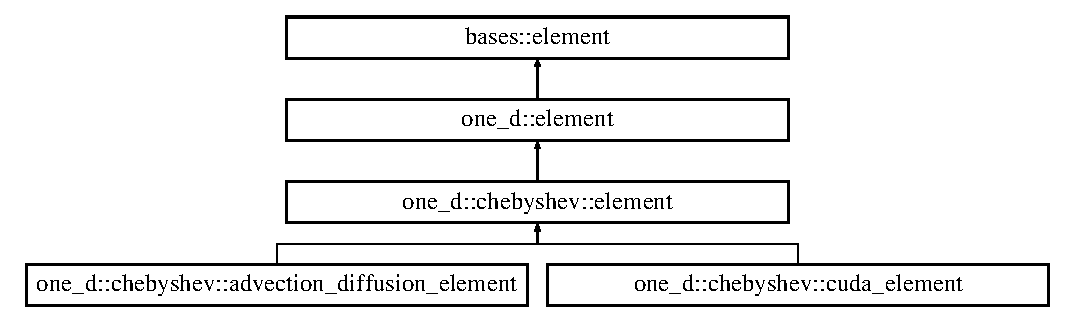
\includegraphics[height=3.875432cm]{classone__d_1_1chebyshev_1_1element}
\end{center}
\end{figure}
\subsection*{Public Member Functions}
\begin{DoxyCompactItemize}
\item 
\hyperlink{classone__d_1_1chebyshev_1_1element_a28bb81f135c419b854354ba966a532af}{element} (int i\-\_\-n, double i\-\_\-position\-\_\-0, double i\-\_\-position\-\_\-n, int i\-\_\-name, \hyperlink{namespaceio_a1c55c654666eeece6a9724f453fdbd87}{io\-::parameter\-\_\-map} \&i\-\_\-input\-Params, \hyperlink{classbases_1_1messenger}{bases\-::messenger} $\ast$i\-\_\-messenger\-\_\-ptr, int i\-\_\-flags)
\begin{DoxyCompactList}\small\item\em \end{DoxyCompactList}\item 
virtual void \hyperlink{classone__d_1_1chebyshev_1_1element_a9af801e1cdc7ccfb79500ba7efad4359}{initialize} (int \hyperlink{classbases_1_1element_a52af85c34174ec732a3feb6a7e63fbc6}{name}, double $\ast$initial\-\_\-conditions=N\-U\-L\-L)
\begin{DoxyCompactList}\small\item\em Initialize the scalar name. \end{DoxyCompactList}\end{DoxyCompactItemize}
\subsection*{Additional Inherited Members}


\subsection{Detailed Description}
A Chebyshev implementation of the 1\-D element class. 



 

\subsection{Constructor \& Destructor Documentation}
\hypertarget{classone__d_1_1chebyshev_1_1element_a28bb81f135c419b854354ba966a532af}{\index{one\-\_\-d\-::chebyshev\-::element@{one\-\_\-d\-::chebyshev\-::element}!element@{element}}
\index{element@{element}!one_d::chebyshev::element@{one\-\_\-d\-::chebyshev\-::element}}
\subsubsection[{element}]{\setlength{\rightskip}{0pt plus 5cm}one\-\_\-d\-::chebyshev\-::element\-::element (
\begin{DoxyParamCaption}
\item[{int}]{i\-\_\-n, }
\item[{double}]{i\-\_\-position\-\_\-0, }
\item[{double}]{i\-\_\-position\-\_\-n, }
\item[{int}]{i\-\_\-name, }
\item[{{\bf io\-::parameter\-\_\-map} \&}]{i\-\_\-input\-Params, }
\item[{{\bf bases\-::messenger} $\ast$}]{i\-\_\-messenger\-\_\-ptr, }
\item[{int}]{i\-\_\-flags}
\end{DoxyParamCaption}
)\hspace{0.3cm}{\ttfamily [inline]}}}\label{classone__d_1_1chebyshev_1_1element_a28bb81f135c419b854354ba966a532af}






 

 
\begin{DoxyParams}{Parameters}
{\em i\-\_\-n} & The number of data elements in each scalar \\
\hline
{\em i\-\_\-position\-\_\-0} & The double position of index excess\-\_\-0 \\
\hline
{\em i\-\_\-position\-\_\-n} & The double position of index n -\/ 1 -\/ excess\-\_\-n \\
\hline
\end{DoxyParams}


 
\begin{DoxyParams}{Parameters}
{\em i\-\_\-name} & The string representation of the element \\
\hline
{\em n\-\_\-boundaries} & The integer number of boundaries (must be a multiple of 2) \\
\hline
{\em i\-\_\-input\-Params} & The parameter object that contains the input parameters of the run \\
\hline
{\em i\-\_\-messenger\-\_\-ptr} & A pointer to a messenger object \\
\hline
{\em i\-\_\-flags} & An integer set of execution flags \\
\hline
\end{DoxyParams}


\subsection{Member Function Documentation}
\hypertarget{classone__d_1_1chebyshev_1_1element_a9af801e1cdc7ccfb79500ba7efad4359}{\index{one\-\_\-d\-::chebyshev\-::element@{one\-\_\-d\-::chebyshev\-::element}!initialize@{initialize}}
\index{initialize@{initialize}!one_d::chebyshev::element@{one\-\_\-d\-::chebyshev\-::element}}
\subsubsection[{initialize}]{\setlength{\rightskip}{0pt plus 5cm}virtual void one\-\_\-d\-::chebyshev\-::element\-::initialize (
\begin{DoxyParamCaption}
\item[{int}]{name, }
\item[{double $\ast$}]{initial\-\_\-conditions = {\ttfamily NULL}}
\end{DoxyParamCaption}
)\hspace{0.3cm}{\ttfamily [inline]}, {\ttfamily [virtual]}}}\label{classone__d_1_1chebyshev_1_1element_a9af801e1cdc7ccfb79500ba7efad4359}


Initialize the scalar name. 



 

 

 
\begin{DoxyParams}{Parameters}
{\em name} & The integer name index to be initialized \\
\hline
{\em initial\-\_\-conditions} & The double array of initial conditions \\
\hline
\end{DoxyParams}


Reimplemented from \hyperlink{classone__d_1_1element_ad6885917730b12fa85d698850184cd4f}{one\-\_\-d\-::element}.



The documentation for this class was generated from the following file\-:\begin{DoxyCompactItemize}
\item 
/\-Users/justinbrown/\-Dropbox/spectral\-\_\-element/src/one\-\_\-d/\hyperlink{element__one__d_8hpp}{element\-\_\-one\-\_\-d.\-hpp}\end{DoxyCompactItemize}

\hypertarget{classone__d_1_1element}{\section{one\-\_\-d\-:\-:element Class Reference}
\label{classone__d_1_1element}\index{one\-\_\-d\-::element@{one\-\_\-d\-::element}}
}


The 1\-D base element class.  




{\ttfamily \#include $<$element\-\_\-one\-\_\-d.\-hpp$>$}

Inheritance diagram for one\-\_\-d\-:\-:element\-:\begin{figure}[H]
\begin{center}
\leavevmode
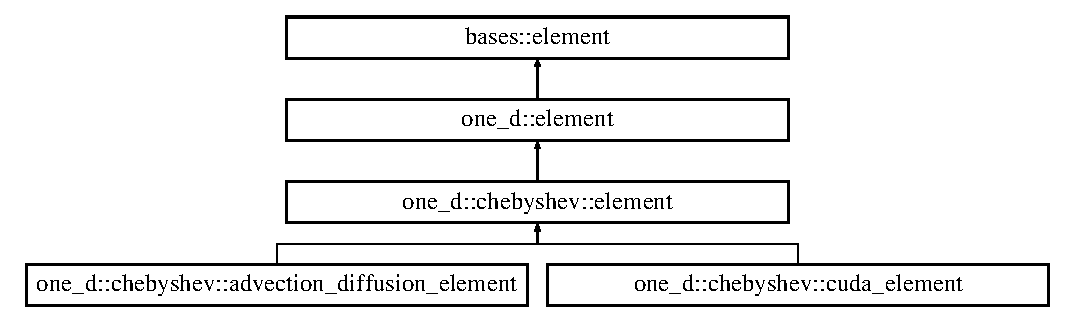
\includegraphics[height=3.875432cm]{classone__d_1_1element}
\end{center}
\end{figure}
\subsection*{Public Member Functions}
\begin{DoxyCompactItemize}
\item 
\hyperlink{classone__d_1_1element_aff9332f16ab0c55ab7cc2f4456ea58d2}{element} (int i\-\_\-n, double i\-\_\-position\-\_\-0, double i\-\_\-position\-\_\-n, int i\-\_\-name, \hyperlink{namespaceio_a1c55c654666eeece6a9724f453fdbd87}{io\-::parameter\-\_\-map} \&i\-\_\-input\-Params, \hyperlink{classbases_1_1messenger}{bases\-::messenger} $\ast$i\-\_\-messenger\-\_\-ptr, int i\-\_\-flags)
\begin{DoxyCompactList}\small\item\em \end{DoxyCompactList}\item 
double \& \hyperlink{classone__d_1_1element_a1d3fa9f4c9f6aacc378f1a71f2729825}{operator\mbox{[}$\,$\mbox{]}} (int \hyperlink{classbases_1_1element_a52af85c34174ec732a3feb6a7e63fbc6}{name})
\begin{DoxyCompactList}\small\item\em Get the double reference to the named scalar. \end{DoxyCompactList}\item 
virtual void \hyperlink{classone__d_1_1element_ad6885917730b12fa85d698850184cd4f}{initialize} (int \hyperlink{classbases_1_1element_a52af85c34174ec732a3feb6a7e63fbc6}{name}, double $\ast$initial\-\_\-conditions=N\-U\-L\-L)
\begin{DoxyCompactList}\small\item\em Initialize the scalar name. \end{DoxyCompactList}\item 
void \hyperlink{classone__d_1_1element_a14ad15e9b835116cd90947c9305725d9}{explicit\-\_\-reset} ()
\begin{DoxyCompactList}\small\item\em Reset every scalar index $<$ 0 and converts to spectral space. \end{DoxyCompactList}\item 
void \hyperlink{classone__d_1_1element_a0d441c27c008871174b291b191f67323}{execute\-\_\-boundaries} ()
\begin{DoxyCompactList}\small\item\em Execute the boundary conditions. \end{DoxyCompactList}\end{DoxyCompactItemize}
\subsection*{Protected Attributes}
\begin{DoxyCompactItemize}
\item 
\hypertarget{classone__d_1_1element_abffb6235b8bcf6e2085ad7dde0c5be3c}{int \hyperlink{classone__d_1_1element_abffb6235b8bcf6e2085ad7dde0c5be3c}{n}}\label{classone__d_1_1element_abffb6235b8bcf6e2085ad7dde0c5be3c}

\begin{DoxyCompactList}\small\item\em The number of elements in each 1\-D array. \end{DoxyCompactList}\item 
\hypertarget{classone__d_1_1element_ad3c5a49b063ecaa54da15a5ff149ad39}{double \hyperlink{classone__d_1_1element_ad3c5a49b063ecaa54da15a5ff149ad39}{position\-\_\-0}}\label{classone__d_1_1element_ad3c5a49b063ecaa54da15a5ff149ad39}

\begin{DoxyCompactList}\small\item\em The double position of index 0. \end{DoxyCompactList}\item 
\hypertarget{classone__d_1_1element_aa9c1febb4303b52f9390e0b198bd8334}{double \hyperlink{classone__d_1_1element_aa9c1febb4303b52f9390e0b198bd8334}{position\-\_\-n}}\label{classone__d_1_1element_aa9c1febb4303b52f9390e0b198bd8334}

\begin{DoxyCompactList}\small\item\em The double position of index n -\/ 1. \end{DoxyCompactList}\item 
\hypertarget{classone__d_1_1element_abc6399df360c45095f825f8cc33c4016}{std\-::vector$<$ int $>$ \hyperlink{classone__d_1_1element_abc6399df360c45095f825f8cc33c4016}{cell}}\label{classone__d_1_1element_abc6399df360c45095f825f8cc33c4016}

\begin{DoxyCompactList}\small\item\em An integer array for tracking each cell number for output. \end{DoxyCompactList}\item 
\hypertarget{classone__d_1_1element_a5a748296569f85cf4d904e0d17aa6388}{std\-::map$<$ int, std\-::vector\\*
$<$ double $>$ $>$ \hyperlink{classone__d_1_1element_a5a748296569f85cf4d904e0d17aa6388}{scalars}}\label{classone__d_1_1element_a5a748296569f85cf4d904e0d17aa6388}

\begin{DoxyCompactList}\small\item\em A vector of scalar vectors. \end{DoxyCompactList}\item 
\hypertarget{classone__d_1_1element_a9f3230a0f72c358b6d2188645cb4058f}{std\-::map$<$ int, double $>$ \hyperlink{classone__d_1_1element_a9f3230a0f72c358b6d2188645cb4058f}{fixed\-\_\-points\-\_\-0}}\label{classone__d_1_1element_a9f3230a0f72c358b6d2188645cb4058f}

\begin{DoxyCompactList}\small\item\em The initial values of the scalars at index 0. \end{DoxyCompactList}\item 
\hypertarget{classone__d_1_1element_a0b44d23843f57cd3c924e07816685bad}{std\-::map$<$ int, double $>$ \hyperlink{classone__d_1_1element_a0b44d23843f57cd3c924e07816685bad}{fixed\-\_\-points\-\_\-n}}\label{classone__d_1_1element_a0b44d23843f57cd3c924e07816685bad}

\begin{DoxyCompactList}\small\item\em The initial values of the scalars at index n -\/ 1. \end{DoxyCompactList}\end{DoxyCompactItemize}
\subsection*{Additional Inherited Members}


\subsection{Detailed Description}
The 1\-D base element class. 



 A 1\-D implementation of the element base class. This provides the storage, indexing facilities, and failsafe\-\_\-dump output. The plans should be added in a further subclass. 

\subsection{Constructor \& Destructor Documentation}
\hypertarget{classone__d_1_1element_aff9332f16ab0c55ab7cc2f4456ea58d2}{\index{one\-\_\-d\-::element@{one\-\_\-d\-::element}!element@{element}}
\index{element@{element}!one_d::element@{one\-\_\-d\-::element}}
\subsubsection[{element}]{\setlength{\rightskip}{0pt plus 5cm}one\-\_\-d\-::element\-::element (
\begin{DoxyParamCaption}
\item[{int}]{i\-\_\-n, }
\item[{double}]{i\-\_\-position\-\_\-0, }
\item[{double}]{i\-\_\-position\-\_\-n, }
\item[{int}]{i\-\_\-name, }
\item[{{\bf io\-::parameter\-\_\-map} \&}]{i\-\_\-input\-Params, }
\item[{{\bf bases\-::messenger} $\ast$}]{i\-\_\-messenger\-\_\-ptr, }
\item[{int}]{i\-\_\-flags}
\end{DoxyParamCaption}
)\hspace{0.3cm}{\ttfamily [inline]}}}\label{classone__d_1_1element_aff9332f16ab0c55ab7cc2f4456ea58d2}






 
\begin{DoxyParams}{Parameters}
{\em i\-\_\-n} & The number of data elements in each scalar \\
\hline
{\em i\-\_\-position\-\_\-0} & The double position of index excess\-\_\-0 \\
\hline
{\em i\-\_\-position\-\_\-n} & The double position of index n -\/ 1 -\/ excess\-\_\-n \\
\hline
\end{DoxyParams}


 
\begin{DoxyParams}{Parameters}
{\em i\-\_\-name} & The string representation of the element \\
\hline
{\em n\-\_\-boundaries} & The integer number of boundaries (must be a multiple of 2) \\
\hline
{\em i\-\_\-input\-Params} & The parameter object that contains the input parameters of the run \\
\hline
{\em i\-\_\-messenger\-\_\-ptr} & A pointer to a messenger object \\
\hline
{\em i\-\_\-flags} & An integer set of execution flags \\
\hline
\end{DoxyParams}


\subsection{Member Function Documentation}
\hypertarget{classone__d_1_1element_a0d441c27c008871174b291b191f67323}{\index{one\-\_\-d\-::element@{one\-\_\-d\-::element}!execute\-\_\-boundaries@{execute\-\_\-boundaries}}
\index{execute\-\_\-boundaries@{execute\-\_\-boundaries}!one_d::element@{one\-\_\-d\-::element}}
\subsubsection[{execute\-\_\-boundaries}]{\setlength{\rightskip}{0pt plus 5cm}void one\-\_\-d\-::element\-::execute\-\_\-boundaries (
\begin{DoxyParamCaption}
{}
\end{DoxyParamCaption}
)\hspace{0.3cm}{\ttfamily [inline]}, {\ttfamily [virtual]}}}\label{classone__d_1_1element_a0d441c27c008871174b291b191f67323}


Execute the boundary conditions. 



 

 In general, this should be overwritten in subclasses.

T\-O\-D\-O I'm not entirely enthused about this method. 

Implements \hyperlink{classbases_1_1element_a86a15277a82abbc28ba75f67817e170a}{bases\-::element}.

\hypertarget{classone__d_1_1element_a14ad15e9b835116cd90947c9305725d9}{\index{one\-\_\-d\-::element@{one\-\_\-d\-::element}!explicit\-\_\-reset@{explicit\-\_\-reset}}
\index{explicit\-\_\-reset@{explicit\-\_\-reset}!one_d::element@{one\-\_\-d\-::element}}
\subsubsection[{explicit\-\_\-reset}]{\setlength{\rightskip}{0pt plus 5cm}void one\-\_\-d\-::element\-::explicit\-\_\-reset (
\begin{DoxyParamCaption}
{}
\end{DoxyParamCaption}
)\hspace{0.3cm}{\ttfamily [inline]}, {\ttfamily [virtual]}}}\label{classone__d_1_1element_a14ad15e9b835116cd90947c9305725d9}


Reset every scalar index $<$ 0 and converts to spectral space. 



 

 At the beginning of each timestep, all scalars with index $<$ 0 should be reset (e.\-g. the right hand sides of equations have index $<$ 0). This must be overwritten in a subclass, which should likely call the base method. The base method converts from normal space to spectral space if necessary. 

Reimplemented from \hyperlink{classbases_1_1element_ac2a829e5dc54ab249d8b567f608e7f69}{bases\-::element}.

\hypertarget{classone__d_1_1element_ad6885917730b12fa85d698850184cd4f}{\index{one\-\_\-d\-::element@{one\-\_\-d\-::element}!initialize@{initialize}}
\index{initialize@{initialize}!one_d::element@{one\-\_\-d\-::element}}
\subsubsection[{initialize}]{\setlength{\rightskip}{0pt plus 5cm}virtual void one\-\_\-d\-::element\-::initialize (
\begin{DoxyParamCaption}
\item[{int}]{name, }
\item[{double $\ast$}]{initial\-\_\-conditions = {\ttfamily NULL}}
\end{DoxyParamCaption}
)\hspace{0.3cm}{\ttfamily [inline]}, {\ttfamily [virtual]}}}\label{classone__d_1_1element_ad6885917730b12fa85d698850184cd4f}


Initialize the scalar name. 



 

 
\begin{DoxyParams}{Parameters}
{\em name} & The integer name index to be initialized \\
\hline
{\em initial\-\_\-conditions} & The double array of initial conditions \\
\hline
\end{DoxyParams}


Implements \hyperlink{classbases_1_1element_a8c0350a45f7aff09ba8ebbfb2a789027}{bases\-::element}.



Reimplemented in \hyperlink{classone__d_1_1chebyshev_1_1element_a9af801e1cdc7ccfb79500ba7efad4359}{one\-\_\-d\-::chebyshev\-::element}.

\hypertarget{classone__d_1_1element_a1d3fa9f4c9f6aacc378f1a71f2729825}{\index{one\-\_\-d\-::element@{one\-\_\-d\-::element}!operator\mbox{[}$\,$\mbox{]}@{operator[]}}
\index{operator\mbox{[}$\,$\mbox{]}@{operator[]}!one_d::element@{one\-\_\-d\-::element}}
\subsubsection[{operator[]}]{\setlength{\rightskip}{0pt plus 5cm}double\& one\-\_\-d\-::element\-::operator\mbox{[}$\,$\mbox{]} (
\begin{DoxyParamCaption}
\item[{int}]{name}
\end{DoxyParamCaption}
)\hspace{0.3cm}{\ttfamily [inline]}, {\ttfamily [virtual]}}}\label{classone__d_1_1element_a1d3fa9f4c9f6aacc378f1a71f2729825}


Get the double reference to the named scalar. 



 
\begin{DoxyParams}{Parameters}
{\em name} & The integer name from the index enumeration\\
\hline
\end{DoxyParams}
\begin{DoxyReturn}{Returns}
A double reference to the first element of the named scalar 
\end{DoxyReturn}


Implements \hyperlink{classbases_1_1element_a4ae6c42893603fc086c5c207e236f9d8}{bases\-::element}.



The documentation for this class was generated from the following file\-:\begin{DoxyCompactItemize}
\item 
/\-Users/justinbrown/\-Dropbox/spectral\-\_\-element/src/one\-\_\-d/\hyperlink{element__one__d_8hpp}{element\-\_\-one\-\_\-d.\-hpp}\end{DoxyCompactItemize}

\hypertarget{classone__d_1_1chebyshev_1_1explicit__diffusion}{\section{one\-\_\-d\-:\-:chebyshev\-:\-:explicit\-\_\-diffusion Class Reference}
\label{classone__d_1_1chebyshev_1_1explicit__diffusion}\index{one\-\_\-d\-::chebyshev\-::explicit\-\_\-diffusion@{one\-\_\-d\-::chebyshev\-::explicit\-\_\-diffusion}}
}


Implementation of explicit diffusion for data expressed as a sum of orthogonal functions in 1\-D.  




{\ttfamily \#include $<$diffusion\-\_\-one\-\_\-d.\-hpp$>$}

Inheritance diagram for one\-\_\-d\-:\-:chebyshev\-:\-:explicit\-\_\-diffusion\-:\begin{figure}[H]
\begin{center}
\leavevmode
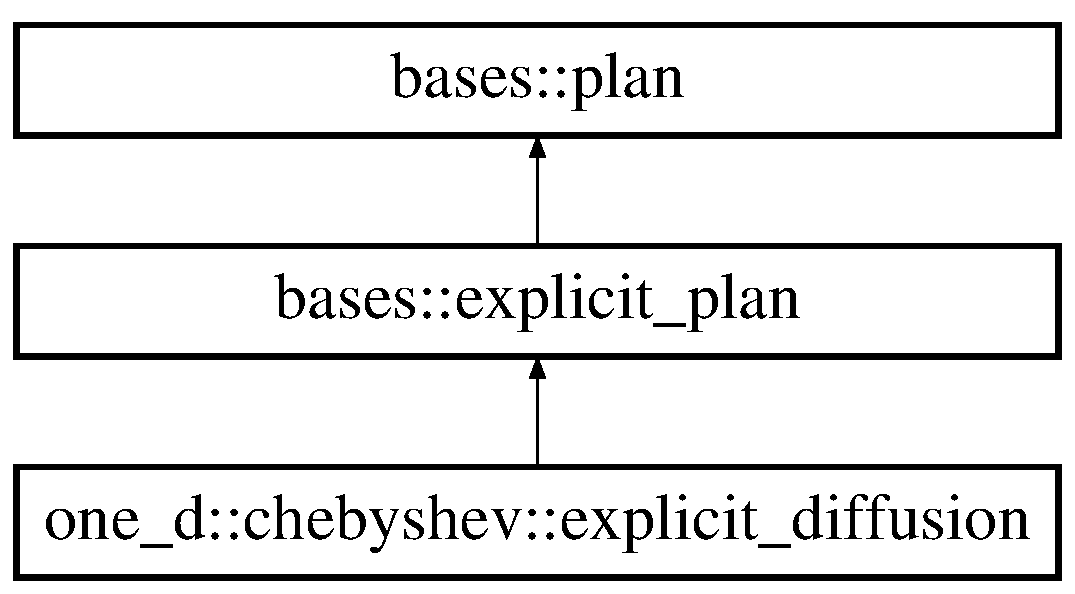
\includegraphics[height=3.000000cm]{classone__d_1_1chebyshev_1_1explicit__diffusion}
\end{center}
\end{figure}
\subsection*{Public Member Functions}
\begin{DoxyCompactItemize}
\item 
\hyperlink{classone__d_1_1chebyshev_1_1explicit__diffusion_a5b7347acb85ad5fcb1c76adb10dc20fa}{explicit\-\_\-diffusion} (\hyperlink{classbases_1_1element}{bases\-::element} $\ast$i\-\_\-element\-\_\-ptr, double i\-\_\-coeff, int i\-\_\-n, \hyperlink{classbases_1_1collocation__grid}{bases\-::collocation\-\_\-grid} $\ast$i\-\_\-grid, int i\-\_\-name\-\_\-in, int i\-\_\-name\-\_\-out=null, int i\-\_\-flags=0x00)
\begin{DoxyCompactList}\small\item\em \end{DoxyCompactList}\item 
void \hyperlink{classone__d_1_1chebyshev_1_1explicit__diffusion_a2a6de638d550ecd781c74d7ef35dd866}{execute} ()
\begin{DoxyCompactList}\small\item\em Operate the plan on the data arrays contained in the class. \end{DoxyCompactList}\end{DoxyCompactItemize}
\subsection*{Additional Inherited Members}


\subsection{Detailed Description}
Implementation of explicit diffusion for data expressed as a sum of orthogonal functions in 1\-D. 



 This implementation calculates the derivatives at the current time 

\subsection{Constructor \& Destructor Documentation}
\hypertarget{classone__d_1_1chebyshev_1_1explicit__diffusion_a5b7347acb85ad5fcb1c76adb10dc20fa}{\index{one\-\_\-d\-::chebyshev\-::explicit\-\_\-diffusion@{one\-\_\-d\-::chebyshev\-::explicit\-\_\-diffusion}!explicit\-\_\-diffusion@{explicit\-\_\-diffusion}}
\index{explicit\-\_\-diffusion@{explicit\-\_\-diffusion}!one_d::chebyshev::explicit_diffusion@{one\-\_\-d\-::chebyshev\-::explicit\-\_\-diffusion}}
\subsubsection[{explicit\-\_\-diffusion}]{\setlength{\rightskip}{0pt plus 5cm}one\-\_\-d\-::chebyshev\-::explicit\-\_\-diffusion\-::explicit\-\_\-diffusion (
\begin{DoxyParamCaption}
\item[{{\bf bases\-::element} $\ast$}]{i\-\_\-element\-\_\-ptr, }
\item[{double}]{i\-\_\-coeff, }
\item[{int}]{i\-\_\-n, }
\item[{{\bf bases\-::collocation\-\_\-grid} $\ast$}]{i\-\_\-grid, }
\item[{int}]{i\-\_\-name\-\_\-in, }
\item[{int}]{i\-\_\-name\-\_\-out = {\ttfamily null}, }
\item[{int}]{i\-\_\-flags = {\ttfamily 0x00}}
\end{DoxyParamCaption}
)}}\label{classone__d_1_1chebyshev_1_1explicit__diffusion_a5b7347acb85ad5fcb1c76adb10dc20fa}






 
\begin{DoxyParams}{Parameters}
{\em i\-\_\-coeff} & A double containing the coefficient in front of the diffusion term in the differential equation \\
\hline
{\em i\-\_\-grid} & a shared pointer to the collocation\-\_\-grid, which must be defined for the second derivative \\
\hline
\end{DoxyParams}


 
\begin{DoxyParams}{Parameters}
{\em i\-\_\-n} & The integer number of elements in the data \\
\hline
{\em i\-\_\-name\-\_\-in} & The integer scalar index of the input \\
\hline
{\em i\-\_\-name\-\_\-out} & The integer scalar index of the output \\
\hline
\end{DoxyParams}


 
\begin{DoxyParams}{Parameters}
{\em i\-\_\-element\-\_\-ptr} & A pointer to the associated element \\
\hline
\end{DoxyParams}


\subsection{Member Function Documentation}
\hypertarget{classone__d_1_1chebyshev_1_1explicit__diffusion_a2a6de638d550ecd781c74d7ef35dd866}{\index{one\-\_\-d\-::chebyshev\-::explicit\-\_\-diffusion@{one\-\_\-d\-::chebyshev\-::explicit\-\_\-diffusion}!execute@{execute}}
\index{execute@{execute}!one_d::chebyshev::explicit_diffusion@{one\-\_\-d\-::chebyshev\-::explicit\-\_\-diffusion}}
\subsubsection[{execute}]{\setlength{\rightskip}{0pt plus 5cm}void one\-\_\-d\-::chebyshev\-::explicit\-\_\-diffusion\-::execute (
\begin{DoxyParamCaption}
{}
\end{DoxyParamCaption}
)\hspace{0.3cm}{\ttfamily [virtual]}}}\label{classone__d_1_1chebyshev_1_1explicit__diffusion_a2a6de638d550ecd781c74d7ef35dd866}


Operate the plan on the data arrays contained in the class. 



 

 

 The plan class serves as a wrapper for this function. 

Reimplemented from \hyperlink{classbases_1_1explicit__plan_a21bcba4d429590031bba41ee2a48a4ef}{bases\-::explicit\-\_\-plan}.



The documentation for this class was generated from the following files\-:\begin{DoxyCompactItemize}
\item 
/\-Users/justinbrown/\-Dropbox/spectral\-\_\-element/src/one\-\_\-d/\hyperlink{diffusion__one__d_8hpp}{diffusion\-\_\-one\-\_\-d.\-hpp}\item 
/\-Users/justinbrown/\-Dropbox/spectral\-\_\-element/src/one\-\_\-d/\hyperlink{diffusion__one__d_8cpp}{diffusion\-\_\-one\-\_\-d.\-cpp}\end{DoxyCompactItemize}

\hypertarget{classbases_1_1explicit__plan}{\section{bases\-:\-:explicit\-\_\-plan Class Reference}
\label{classbases_1_1explicit__plan}\index{bases\-::explicit\-\_\-plan@{bases\-::explicit\-\_\-plan}}
}


A subclass of plan, specific to explicit methods.  




{\ttfamily \#include $<$plan.\-hpp$>$}

Inheritance diagram for bases\-:\-:explicit\-\_\-plan\-:\begin{figure}[H]
\begin{center}
\leavevmode
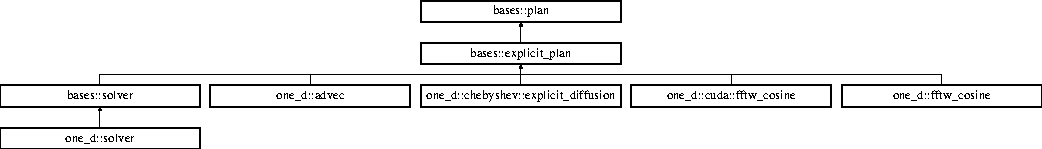
\includegraphics[height=2.008969cm]{classbases_1_1explicit__plan}
\end{center}
\end{figure}
\subsection*{Public Member Functions}
\begin{DoxyCompactItemize}
\item 
\hyperlink{classbases_1_1explicit__plan_a4c4c1f48e79e10dd6f85610f5814ba7f}{explicit\-\_\-plan} (\hyperlink{classbases_1_1element}{element} $\ast$i\-\_\-element\-\_\-ptr, int i\-\_\-n, int i\-\_\-name\-\_\-in, int i\-\_\-name\-\_\-out=null, int flags=0x00)
\begin{DoxyCompactList}\small\item\em \end{DoxyCompactList}\item 
virtual void \hyperlink{classbases_1_1explicit__plan_a21bcba4d429590031bba41ee2a48a4ef}{execute} ()
\begin{DoxyCompactList}\small\item\em Operate the plan on the data arrays contained in the class. \end{DoxyCompactList}\end{DoxyCompactItemize}
\subsection*{Protected Attributes}
\begin{DoxyCompactItemize}
\item 
\hypertarget{classbases_1_1explicit__plan_a6acccce0b2ef4489b411a264cab019c9}{int \hyperlink{classbases_1_1explicit__plan_a6acccce0b2ef4489b411a264cab019c9}{n}}\label{classbases_1_1explicit__plan_a6acccce0b2ef4489b411a264cab019c9}

\begin{DoxyCompactList}\small\item\em An integer number of data elements (grid points) that collocation\-\_\-1\-D will be built to handle. \end{DoxyCompactList}\item 
\hypertarget{classbases_1_1explicit__plan_a8faf976ec6c01951dd6d5e7421630184}{double $\ast$ \hyperlink{classbases_1_1explicit__plan_a8faf976ec6c01951dd6d5e7421630184}{data\-\_\-in}}\label{classbases_1_1explicit__plan_a8faf976ec6c01951dd6d5e7421630184}

\begin{DoxyCompactList}\small\item\em A double pointer to the input data. \end{DoxyCompactList}\item 
\hypertarget{classbases_1_1explicit__plan_a55946d0b4b1a19da12469447de247b82}{double $\ast$ \hyperlink{classbases_1_1explicit__plan_a55946d0b4b1a19da12469447de247b82}{data\-\_\-out}}\label{classbases_1_1explicit__plan_a55946d0b4b1a19da12469447de247b82}

\begin{DoxyCompactList}\small\item\em A double pointer to the output data. \end{DoxyCompactList}\end{DoxyCompactItemize}


\subsection{Detailed Description}
A subclass of plan, specific to explicit methods. 



 These plans take input and produce output. 

\subsection{Constructor \& Destructor Documentation}
\hypertarget{classbases_1_1explicit__plan_a4c4c1f48e79e10dd6f85610f5814ba7f}{\index{bases\-::explicit\-\_\-plan@{bases\-::explicit\-\_\-plan}!explicit\-\_\-plan@{explicit\-\_\-plan}}
\index{explicit\-\_\-plan@{explicit\-\_\-plan}!bases::explicit_plan@{bases\-::explicit\-\_\-plan}}
\subsubsection[{explicit\-\_\-plan}]{\setlength{\rightskip}{0pt plus 5cm}bases\-::explicit\-\_\-plan\-::explicit\-\_\-plan (
\begin{DoxyParamCaption}
\item[{{\bf element} $\ast$}]{i\-\_\-element\-\_\-ptr, }
\item[{int}]{i\-\_\-n, }
\item[{int}]{i\-\_\-name\-\_\-in, }
\item[{int}]{i\-\_\-name\-\_\-out = {\ttfamily null}, }
\item[{int}]{flags = {\ttfamily 0x00}}
\end{DoxyParamCaption}
)}}\label{classbases_1_1explicit__plan_a4c4c1f48e79e10dd6f85610f5814ba7f}






 
\begin{DoxyParams}{Parameters}
{\em i\-\_\-n} & The integer number of elements in the data \\
\hline
{\em i\-\_\-name\-\_\-in} & The integer scalar index of the input \\
\hline
{\em i\-\_\-name\-\_\-out} & The integer scalar index of the output \\
\hline
\end{DoxyParams}


 
\begin{DoxyParams}{Parameters}
{\em i\-\_\-element\-\_\-ptr} & A pointer to the associated element \\
\hline
\end{DoxyParams}


\subsection{Member Function Documentation}
\hypertarget{classbases_1_1explicit__plan_a21bcba4d429590031bba41ee2a48a4ef}{\index{bases\-::explicit\-\_\-plan@{bases\-::explicit\-\_\-plan}!execute@{execute}}
\index{execute@{execute}!bases::explicit_plan@{bases\-::explicit\-\_\-plan}}
\subsubsection[{execute}]{\setlength{\rightskip}{0pt plus 5cm}void bases\-::explicit\-\_\-plan\-::execute (
\begin{DoxyParamCaption}
{}
\end{DoxyParamCaption}
)\hspace{0.3cm}{\ttfamily [virtual]}}}\label{classbases_1_1explicit__plan_a21bcba4d429590031bba41ee2a48a4ef}


Operate the plan on the data arrays contained in the class. 



 

 The plan class serves as a wrapper for this function. 

Reimplemented from \hyperlink{classbases_1_1plan_a85d7e7f7a04ac8213ea57bde32db34c2}{bases\-::plan}.



Reimplemented in \hyperlink{classone__d_1_1solver_a7c28bd733cb3c3849afe1773974eb4f6}{one\-\_\-d\-::solver}, \hyperlink{classone__d_1_1chebyshev_1_1explicit__diffusion_a2a6de638d550ecd781c74d7ef35dd866}{one\-\_\-d\-::chebyshev\-::explicit\-\_\-diffusion}, \hyperlink{classone__d_1_1cuda_1_1fftw__cosine_a557fc154a9e6ffe9a8179667b66901dc}{one\-\_\-d\-::cuda\-::fftw\-\_\-cosine}, \hyperlink{classone__d_1_1fftw__cosine_aa8b0befe7b047feb004b2c41644a2fa4}{one\-\_\-d\-::fftw\-\_\-cosine}, \hyperlink{classbases_1_1solver_a8adf4c428bf4322a664c811073b491e1}{bases\-::solver}, and \hyperlink{classone__d_1_1advec_a1811538aec2a23cc27ef87fbce5dec8c}{one\-\_\-d\-::advec}.



The documentation for this class was generated from the following files\-:\begin{DoxyCompactItemize}
\item 
/\-Users/justinbrown/\-Dropbox/spectral\-\_\-element/src/bases/\hyperlink{plan_8hpp}{plan.\-hpp}\item 
/\-Users/justinbrown/\-Dropbox/spectral\-\_\-element/src/bases/\hyperlink{plan_8cpp}{plan.\-cpp}\end{DoxyCompactItemize}

\hypertarget{classone__d_1_1fftw__cosine}{\section{one\-\_\-d\-:\-:fftw\-\_\-cosine Class Reference}
\label{classone__d_1_1fftw__cosine}\index{one\-\_\-d\-::fftw\-\_\-cosine@{one\-\_\-d\-::fftw\-\_\-cosine}}
}


 




{\ttfamily \#include $<$fftw\-\_\-one\-\_\-d.\-hpp$>$}

Inheritance diagram for one\-\_\-d\-:\-:fftw\-\_\-cosine\-:\begin{figure}[H]
\begin{center}
\leavevmode
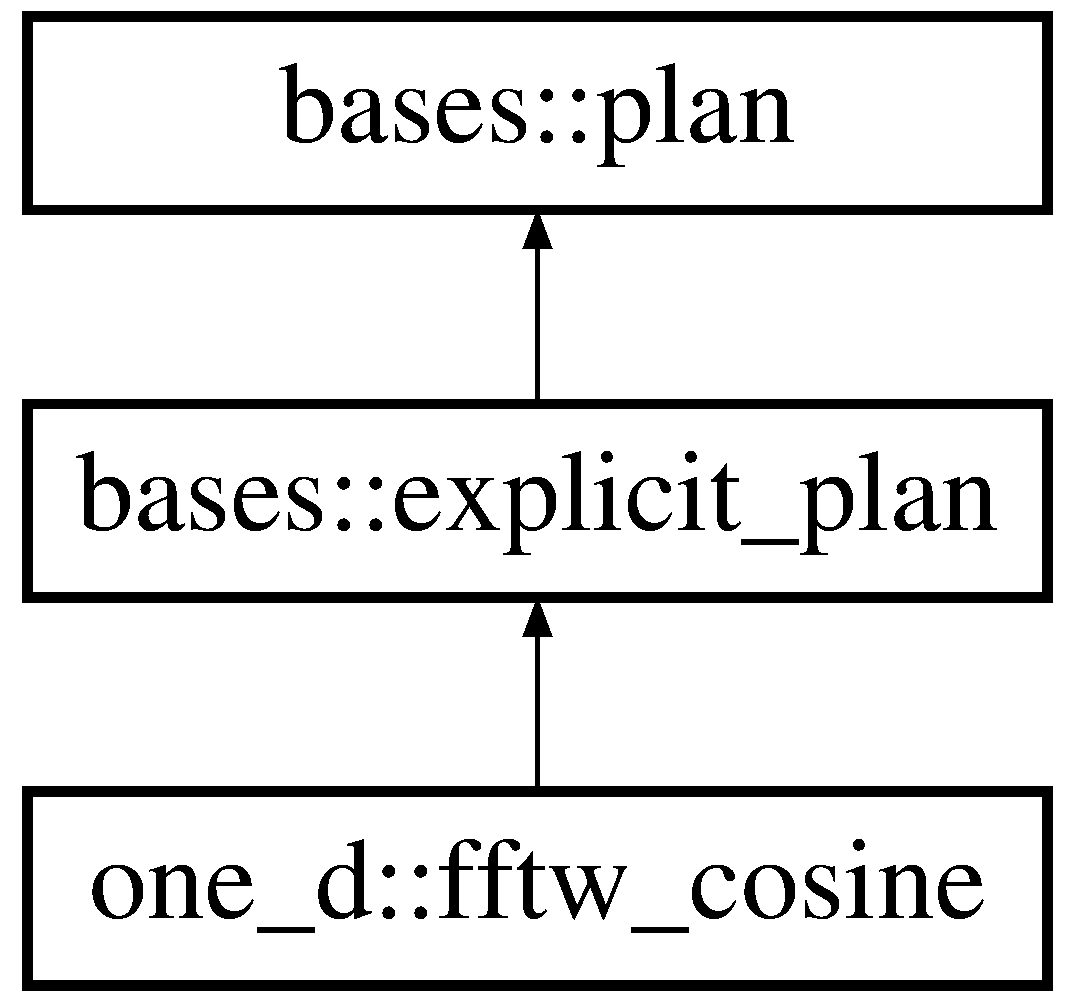
\includegraphics[height=3.000000cm]{classone__d_1_1fftw__cosine}
\end{center}
\end{figure}
\subsection*{Public Member Functions}
\begin{DoxyCompactItemize}
\item 
\hyperlink{classone__d_1_1fftw__cosine_aa74ba6cf6ada1c3a1573137328dbc9a0}{fftw\-\_\-cosine} (\hyperlink{classbases_1_1element}{bases\-::element} $\ast$i\-\_\-element\-\_\-ptr, int i\-\_\-n, int i\-\_\-name\-\_\-in, int i\-\_\-name\-\_\-out=null, int i\-\_\-flags=0x00)
\begin{DoxyCompactList}\small\item\em \end{DoxyCompactList}\item 
void \hyperlink{classone__d_1_1fftw__cosine_aa8b0befe7b047feb004b2c41644a2fa4}{execute} ()
\begin{DoxyCompactList}\small\item\em \end{DoxyCompactList}\end{DoxyCompactItemize}
\subsection*{Additional Inherited Members}


\subsection{Detailed Description}




 An implementation of the transform class using F\-F\-T\-W3. 

\subsection{Constructor \& Destructor Documentation}
\hypertarget{classone__d_1_1fftw__cosine_aa74ba6cf6ada1c3a1573137328dbc9a0}{\index{one\-\_\-d\-::fftw\-\_\-cosine@{one\-\_\-d\-::fftw\-\_\-cosine}!fftw\-\_\-cosine@{fftw\-\_\-cosine}}
\index{fftw\-\_\-cosine@{fftw\-\_\-cosine}!one_d::fftw_cosine@{one\-\_\-d\-::fftw\-\_\-cosine}}
\subsubsection[{fftw\-\_\-cosine}]{\setlength{\rightskip}{0pt plus 5cm}one\-\_\-d\-::fftw\-\_\-cosine\-::fftw\-\_\-cosine (
\begin{DoxyParamCaption}
\item[{{\bf bases\-::element} $\ast$}]{i\-\_\-element\-\_\-ptr, }
\item[{int}]{i\-\_\-n, }
\item[{int}]{i\-\_\-name\-\_\-in, }
\item[{int}]{i\-\_\-name\-\_\-out = {\ttfamily null}, }
\item[{int}]{i\-\_\-flags = {\ttfamily 0x00}}
\end{DoxyParamCaption}
)\hspace{0.3cm}{\ttfamily [inline]}}}\label{classone__d_1_1fftw__cosine_aa74ba6cf6ada1c3a1573137328dbc9a0}






 

\subsection{Member Function Documentation}
\hypertarget{classone__d_1_1fftw__cosine_aa8b0befe7b047feb004b2c41644a2fa4}{\index{one\-\_\-d\-::fftw\-\_\-cosine@{one\-\_\-d\-::fftw\-\_\-cosine}!execute@{execute}}
\index{execute@{execute}!one_d::fftw_cosine@{one\-\_\-d\-::fftw\-\_\-cosine}}
\subsubsection[{execute}]{\setlength{\rightskip}{0pt plus 5cm}void one\-\_\-d\-::fftw\-\_\-cosine\-::execute (
\begin{DoxyParamCaption}
{}
\end{DoxyParamCaption}
)\hspace{0.3cm}{\ttfamily [inline]}, {\ttfamily [virtual]}}}\label{classone__d_1_1fftw__cosine_aa8b0befe7b047feb004b2c41644a2fa4}






 

Reimplemented from \hyperlink{classbases_1_1explicit__plan_a21bcba4d429590031bba41ee2a48a4ef}{bases\-::explicit\-\_\-plan}.



The documentation for this class was generated from the following file\-:\begin{DoxyCompactItemize}
\item 
/\-Users/justinbrown/\-Dropbox/spectral\-\_\-element/src/one\-\_\-d/\hyperlink{fftw__one__d_8hpp}{fftw\-\_\-one\-\_\-d.\-hpp}\end{DoxyCompactItemize}

\hypertarget{classone__d_1_1cuda_1_1fftw__cosine}{\section{one\-\_\-d\-:\-:cuda\-:\-:fftw\-\_\-cosine Class Reference}
\label{classone__d_1_1cuda_1_1fftw__cosine}\index{one\-\_\-d\-::cuda\-::fftw\-\_\-cosine@{one\-\_\-d\-::cuda\-::fftw\-\_\-cosine}}
}


A subclass of plan, specific to explicit methods.  




{\ttfamily \#include $<$fftw\-\_\-one\-\_\-d\-\_\-cuda.\-hpp$>$}

Inheritance diagram for one\-\_\-d\-:\-:cuda\-:\-:fftw\-\_\-cosine\-:\begin{figure}[H]
\begin{center}
\leavevmode
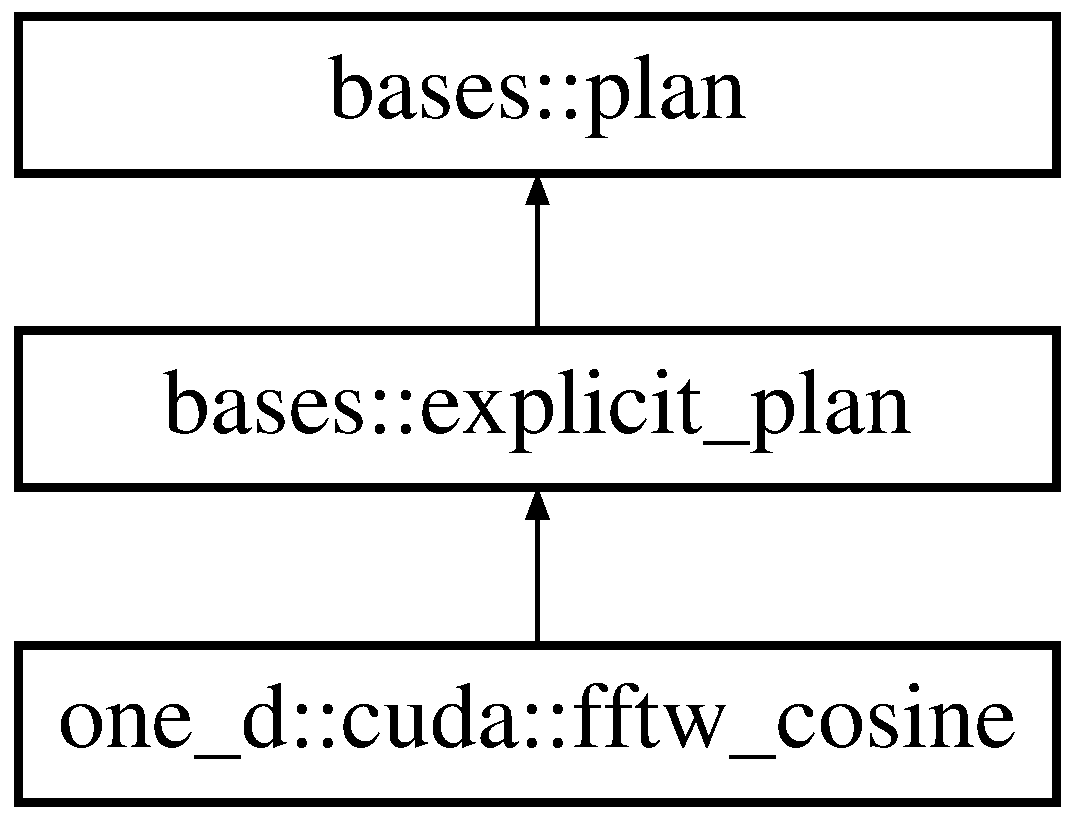
\includegraphics[height=3.000000cm]{classone__d_1_1cuda_1_1fftw__cosine}
\end{center}
\end{figure}
\subsection*{Public Member Functions}
\begin{DoxyCompactItemize}
\item 
\hyperlink{classone__d_1_1cuda_1_1fftw__cosine_a35bf1ddd6e20eb04ab5293c461344919}{fftw\-\_\-cosine} (\hyperlink{classbases_1_1element}{bases\-::element} $\ast$i\-\_\-element\-\_\-ptr, int i\-\_\-n, int i\-\_\-name\-\_\-in, int i\-\_\-name\-\_\-out=null)
\begin{DoxyCompactList}\small\item\em \end{DoxyCompactList}\item 
void \hyperlink{classone__d_1_1cuda_1_1fftw__cosine_a557fc154a9e6ffe9a8179667b66901dc}{execute} ()
\begin{DoxyCompactList}\small\item\em Operate the plan on the data arrays contained in the class. \end{DoxyCompactList}\end{DoxyCompactItemize}
\subsection*{Additional Inherited Members}


\subsection{Detailed Description}
A subclass of plan, specific to explicit methods. 



 An implementation of the transform class using F\-F\-T\-W3. 

\subsection{Constructor \& Destructor Documentation}
\hypertarget{classone__d_1_1cuda_1_1fftw__cosine_a35bf1ddd6e20eb04ab5293c461344919}{\index{one\-\_\-d\-::cuda\-::fftw\-\_\-cosine@{one\-\_\-d\-::cuda\-::fftw\-\_\-cosine}!fftw\-\_\-cosine@{fftw\-\_\-cosine}}
\index{fftw\-\_\-cosine@{fftw\-\_\-cosine}!one_d::cuda::fftw_cosine@{one\-\_\-d\-::cuda\-::fftw\-\_\-cosine}}
\subsubsection[{fftw\-\_\-cosine}]{\setlength{\rightskip}{0pt plus 5cm}one\-\_\-d\-::cuda\-::fftw\-\_\-cosine\-::fftw\-\_\-cosine (
\begin{DoxyParamCaption}
\item[{{\bf bases\-::element} $\ast$}]{i\-\_\-element\-\_\-ptr, }
\item[{int}]{i\-\_\-n, }
\item[{int}]{i\-\_\-name\-\_\-in, }
\item[{int}]{i\-\_\-name\-\_\-out = {\ttfamily null}}
\end{DoxyParamCaption}
)}}\label{classone__d_1_1cuda_1_1fftw__cosine_a35bf1ddd6e20eb04ab5293c461344919}






 

 
\begin{DoxyParams}{Parameters}
{\em i\-\_\-n} & The integer number of elements in the data \\
\hline
{\em i\-\_\-name\-\_\-in} & The integer scalar index of the input \\
\hline
{\em i\-\_\-name\-\_\-out} & The integer scalar index of the output \\
\hline
\end{DoxyParams}


 
\begin{DoxyParams}{Parameters}
{\em i\-\_\-element\-\_\-ptr} & A pointer to the associated element \\
\hline
\end{DoxyParams}


\subsection{Member Function Documentation}
\hypertarget{classone__d_1_1cuda_1_1fftw__cosine_a557fc154a9e6ffe9a8179667b66901dc}{\index{one\-\_\-d\-::cuda\-::fftw\-\_\-cosine@{one\-\_\-d\-::cuda\-::fftw\-\_\-cosine}!execute@{execute}}
\index{execute@{execute}!one_d::cuda::fftw_cosine@{one\-\_\-d\-::cuda\-::fftw\-\_\-cosine}}
\subsubsection[{execute}]{\setlength{\rightskip}{0pt plus 5cm}void one\-\_\-d\-::cuda\-::fftw\-\_\-cosine\-::execute (
\begin{DoxyParamCaption}
{}
\end{DoxyParamCaption}
)\hspace{0.3cm}{\ttfamily [virtual]}}}\label{classone__d_1_1cuda_1_1fftw__cosine_a557fc154a9e6ffe9a8179667b66901dc}


Operate the plan on the data arrays contained in the class. 



 

 

 The plan class serves as a wrapper for this function. 

Reimplemented from \hyperlink{classbases_1_1explicit__plan_a21bcba4d429590031bba41ee2a48a4ef}{bases\-::explicit\-\_\-plan}.



The documentation for this class was generated from the following file\-:\begin{DoxyCompactItemize}
\item 
/\-Users/justinbrown/\-Dropbox/spectral\-\_\-element/src/one\-\_\-d/\hyperlink{fftw__one__d__cuda_8hpp}{fftw\-\_\-one\-\_\-d\-\_\-cuda.\-hpp}\end{DoxyCompactItemize}

\hypertarget{classio_1_1exceptions_1_1file__exception}{\section{io\-:\-:exceptions\-:\-:file\-\_\-exception Class Reference}
\label{classio_1_1exceptions_1_1file__exception}\index{io\-::exceptions\-::file\-\_\-exception@{io\-::exceptions\-::file\-\_\-exception}}
}


This is an exception that can occur when opening files.  




{\ttfamily \#include $<$exceptions.\-hpp$>$}

Inheritance diagram for io\-:\-:exceptions\-:\-:file\-\_\-exception\-:\begin{figure}[H]
\begin{center}
\leavevmode
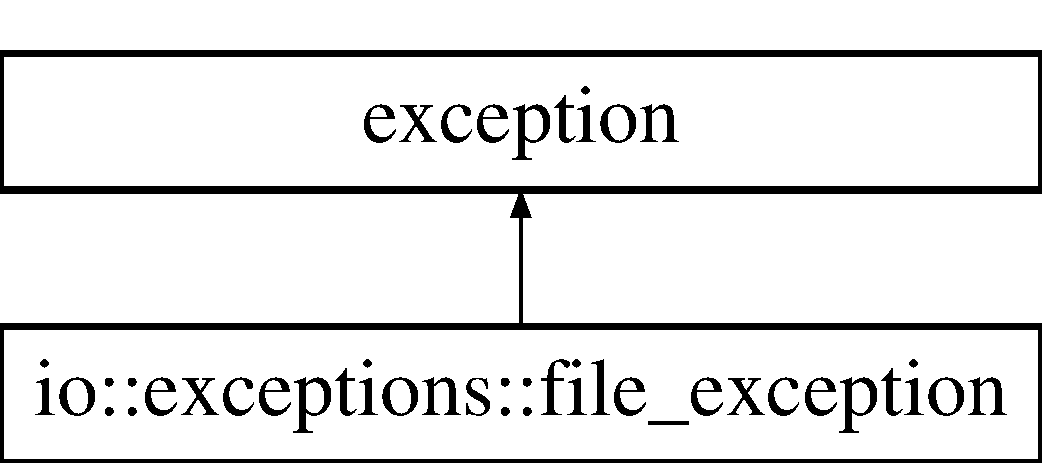
\includegraphics[height=2.000000cm]{classio_1_1exceptions_1_1file__exception}
\end{center}
\end{figure}
\subsection*{Public Member Functions}
\begin{DoxyCompactItemize}
\item 
const char $\ast$ \hyperlink{classio_1_1exceptions_1_1file__exception_ad9313788b0771722c6e2e51ac1ec8a8d}{what} ()
\begin{DoxyCompactList}\small\item\em Describe the nature of the exception. \end{DoxyCompactList}\end{DoxyCompactItemize}


\subsection{Detailed Description}
This is an exception that can occur when opening files. 



 

\subsection{Member Function Documentation}
\hypertarget{classio_1_1exceptions_1_1file__exception_ad9313788b0771722c6e2e51ac1ec8a8d}{\index{io\-::exceptions\-::file\-\_\-exception@{io\-::exceptions\-::file\-\_\-exception}!what@{what}}
\index{what@{what}!io::exceptions::file_exception@{io\-::exceptions\-::file\-\_\-exception}}
\subsubsection[{what}]{\setlength{\rightskip}{0pt plus 5cm}const char$\ast$ io\-::exceptions\-::file\-\_\-exception\-::what (
\begin{DoxyParamCaption}
{}
\end{DoxyParamCaption}
)\hspace{0.3cm}{\ttfamily [inline]}}}\label{classio_1_1exceptions_1_1file__exception_ad9313788b0771722c6e2e51ac1ec8a8d}


Describe the nature of the exception. 



 

The documentation for this class was generated from the following file\-:\begin{DoxyCompactItemize}
\item 
/\-Users/justinbrown/\-Dropbox/spectral\-\_\-element/src/utils/\hyperlink{exceptions_8hpp}{exceptions.\-hpp}\end{DoxyCompactItemize}

\hypertarget{classio_1_1header}{\section{io\-:\-:header Class Reference}
\label{classio_1_1header}\index{io\-::header@{io\-::header}}
}


A base class that is essentially a null header.  




{\ttfamily \#include $<$io.\-hpp$>$}

Inheritance diagram for io\-:\-:header\-:\begin{figure}[H]
\begin{center}
\leavevmode
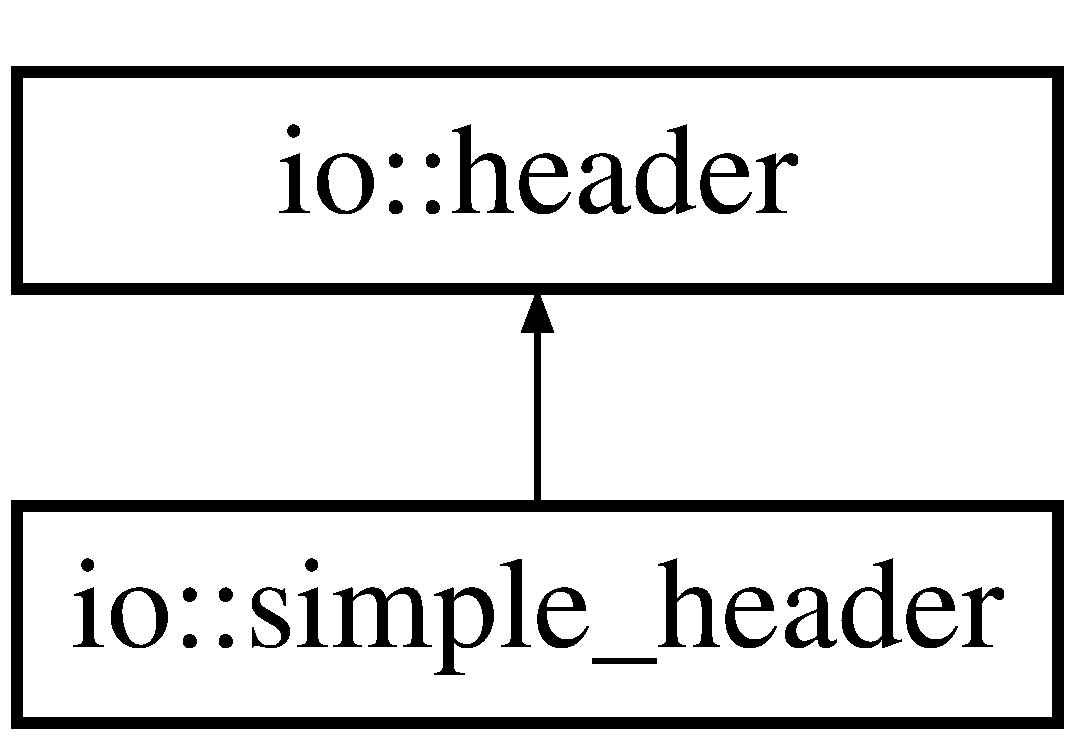
\includegraphics[height=2.000000cm]{classio_1_1header}
\end{center}
\end{figure}
\subsection*{Public Member Functions}
\begin{DoxyCompactItemize}
\item 
virtual std\-::string \hyperlink{classio_1_1header_af7535d58a31712cdfb753ab0f19626f1}{output\-\_\-header} ()
\begin{DoxyCompactList}\small\item\em Method that generates the header for an output object. \end{DoxyCompactList}\end{DoxyCompactItemize}


\subsection{Detailed Description}
A base class that is essentially a null header. 



 Subclasses inheriting from this class should overload the output\-\_\-header method, which outputs a string that will represent the header of the output file. 

\subsection{Member Function Documentation}
\hypertarget{classio_1_1header_af7535d58a31712cdfb753ab0f19626f1}{\index{io\-::header@{io\-::header}!output\-\_\-header@{output\-\_\-header}}
\index{output\-\_\-header@{output\-\_\-header}!io::header@{io\-::header}}
\subsubsection[{output\-\_\-header}]{\setlength{\rightskip}{0pt plus 5cm}virtual std\-::string io\-::header\-::output\-\_\-header (
\begin{DoxyParamCaption}
{}
\end{DoxyParamCaption}
)\hspace{0.3cm}{\ttfamily [inline]}, {\ttfamily [virtual]}}}\label{classio_1_1header_af7535d58a31712cdfb753ab0f19626f1}


Method that generates the header for an output object. 



 This method should be overwritted by subclasses to be replaced with more elaborate headers.

\begin{DoxyReturn}{Returns}
A string which will be used as the header in the associated output 
\end{DoxyReturn}


Reimplemented in \hyperlink{classio_1_1simple__header_a24e9f310d5a022872ef315204e4b0add}{io\-::simple\-\_\-header}.



The documentation for this class was generated from the following file\-:\begin{DoxyCompactItemize}
\item 
/\-Users/justinbrown/\-Dropbox/spectral\-\_\-element/src/utils/\hyperlink{io_8hpp}{io.\-hpp}\end{DoxyCompactItemize}

\hypertarget{classone__d_1_1chebyshev_1_1implicit__diffusion}{\section{one\-\_\-d\-:\-:chebyshev\-:\-:implicit\-\_\-diffusion Class Reference}
\label{classone__d_1_1chebyshev_1_1implicit__diffusion}\index{one\-\_\-d\-::chebyshev\-::implicit\-\_\-diffusion@{one\-\_\-d\-::chebyshev\-::implicit\-\_\-diffusion}}
}


Implementation of implicit diffusion for data expressed as a sum of orthogonal functions in 1\-D.  




{\ttfamily \#include $<$diffusion\-\_\-one\-\_\-d.\-hpp$>$}

Inheritance diagram for one\-\_\-d\-:\-:chebyshev\-:\-:implicit\-\_\-diffusion\-:\begin{figure}[H]
\begin{center}
\leavevmode
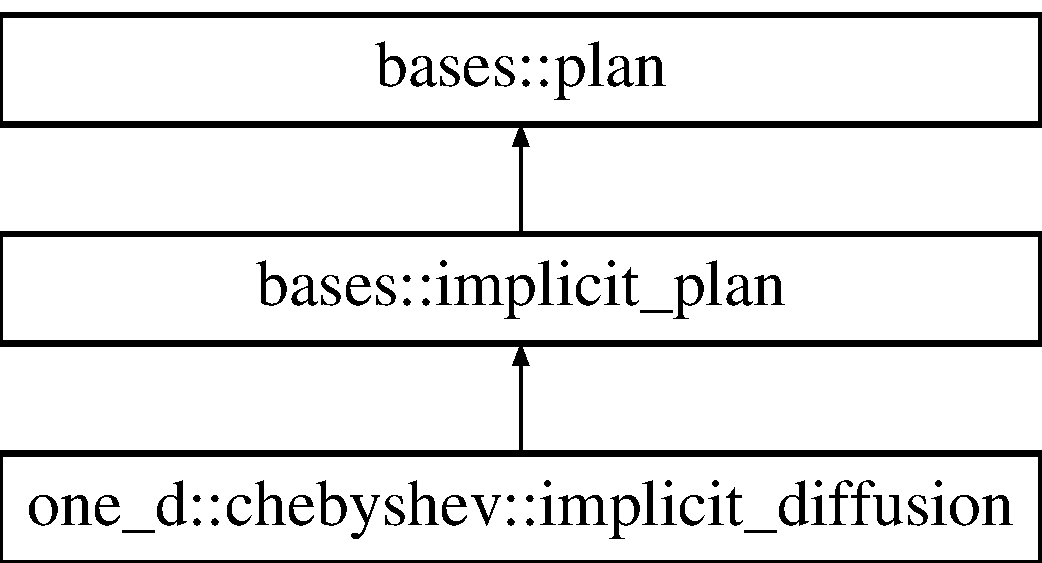
\includegraphics[height=3.000000cm]{classone__d_1_1chebyshev_1_1implicit__diffusion}
\end{center}
\end{figure}
\subsection*{Public Member Functions}
\begin{DoxyCompactItemize}
\item 
\hyperlink{classone__d_1_1chebyshev_1_1implicit__diffusion_a35446cbf70197754a5039cd8bfc3d30e}{implicit\-\_\-diffusion} (\hyperlink{classbases_1_1element}{bases\-::element} $\ast$i\-\_\-element\-\_\-ptr, double i\-\_\-coeff, int i\-\_\-n, \hyperlink{classbases_1_1collocation__grid}{bases\-::collocation\-\_\-grid} $\ast$i\-\_\-grid, double $\ast$i\-\_\-matrix, int i\-\_\-flags=0x00)
\item 
void \hyperlink{classone__d_1_1chebyshev_1_1implicit__diffusion_a5da5289b943a5d3384c7b0341f890125}{execute} ()
\begin{DoxyCompactList}\small\item\em Operate the plan on the data arrays contained in the class. \end{DoxyCompactList}\end{DoxyCompactItemize}
\subsection*{Additional Inherited Members}


\subsection{Detailed Description}
Implementation of implicit diffusion for data expressed as a sum of orthogonal functions in 1\-D. 



 This implementation adds the diffusion terms to the implicit matrix. 

\subsection{Constructor \& Destructor Documentation}
\hypertarget{classone__d_1_1chebyshev_1_1implicit__diffusion_a35446cbf70197754a5039cd8bfc3d30e}{\index{one\-\_\-d\-::chebyshev\-::implicit\-\_\-diffusion@{one\-\_\-d\-::chebyshev\-::implicit\-\_\-diffusion}!implicit\-\_\-diffusion@{implicit\-\_\-diffusion}}
\index{implicit\-\_\-diffusion@{implicit\-\_\-diffusion}!one_d::chebyshev::implicit_diffusion@{one\-\_\-d\-::chebyshev\-::implicit\-\_\-diffusion}}
\subsubsection[{implicit\-\_\-diffusion}]{\setlength{\rightskip}{0pt plus 5cm}one\-\_\-d\-::chebyshev\-::implicit\-\_\-diffusion\-::implicit\-\_\-diffusion (
\begin{DoxyParamCaption}
\item[{{\bf bases\-::element} $\ast$}]{i\-\_\-element\-\_\-ptr, }
\item[{double}]{i\-\_\-coeff, }
\item[{int}]{i\-\_\-n, }
\item[{{\bf bases\-::collocation\-\_\-grid} $\ast$}]{i\-\_\-grid, }
\item[{double $\ast$}]{i\-\_\-matrix, }
\item[{int}]{i\-\_\-flags = {\ttfamily 0x00}}
\end{DoxyParamCaption}
)}}\label{classone__d_1_1chebyshev_1_1implicit__diffusion_a35446cbf70197754a5039cd8bfc3d30e}


 
\begin{DoxyParams}{Parameters}
{\em i\-\_\-coeff} & A double containing the coefficient in front of the diffusion term in the differential equation \\
\hline
{\em i\-\_\-grid} & a shared pointer to the collocation\-\_\-grid, which must be defined for the second derivative\\
\hline
\end{DoxyParams}


 
\begin{DoxyParams}{Parameters}
{\em i\-\_\-n} & The integer number of elements in a row of the square i\-\_\-matrix \\
\hline
{\em i\-\_\-grid} & A shared pointer to the collocation grid object \\
\hline
{\em i\-\_\-matrix} & The double matrix to be updated \\
\hline
\end{DoxyParams}


 
\begin{DoxyParams}{Parameters}
{\em i\-\_\-element\-\_\-ptr} & A pointer to the associated element \\
\hline
\end{DoxyParams}


\subsection{Member Function Documentation}
\hypertarget{classone__d_1_1chebyshev_1_1implicit__diffusion_a5da5289b943a5d3384c7b0341f890125}{\index{one\-\_\-d\-::chebyshev\-::implicit\-\_\-diffusion@{one\-\_\-d\-::chebyshev\-::implicit\-\_\-diffusion}!execute@{execute}}
\index{execute@{execute}!one_d::chebyshev::implicit_diffusion@{one\-\_\-d\-::chebyshev\-::implicit\-\_\-diffusion}}
\subsubsection[{execute}]{\setlength{\rightskip}{0pt plus 5cm}void one\-\_\-d\-::chebyshev\-::implicit\-\_\-diffusion\-::execute (
\begin{DoxyParamCaption}
{}
\end{DoxyParamCaption}
)\hspace{0.3cm}{\ttfamily [virtual]}}}\label{classone__d_1_1chebyshev_1_1implicit__diffusion_a5da5289b943a5d3384c7b0341f890125}


Operate the plan on the data arrays contained in the class. 



 

 

 The plan class serves as a wrapper for this function. 

Reimplemented from \hyperlink{classbases_1_1implicit__plan_a564bcb2be88ca9abe77c981d77d58d74}{bases\-::implicit\-\_\-plan}.



The documentation for this class was generated from the following files\-:\begin{DoxyCompactItemize}
\item 
/\-Users/justinbrown/\-Dropbox/spectral\-\_\-element/src/one\-\_\-d/\hyperlink{diffusion__one__d_8hpp}{diffusion\-\_\-one\-\_\-d.\-hpp}\item 
/\-Users/justinbrown/\-Dropbox/spectral\-\_\-element/src/one\-\_\-d/\hyperlink{diffusion__one__d_8cpp}{diffusion\-\_\-one\-\_\-d.\-cpp}\end{DoxyCompactItemize}

\hypertarget{classbases_1_1implicit__plan}{\section{bases\-:\-:implicit\-\_\-plan Class Reference}
\label{classbases_1_1implicit__plan}\index{bases\-::implicit\-\_\-plan@{bases\-::implicit\-\_\-plan}}
}


A subclass of plan, specific to implicit methods.  




{\ttfamily \#include $<$plan.\-hpp$>$}

Inheritance diagram for bases\-:\-:implicit\-\_\-plan\-:\begin{figure}[H]
\begin{center}
\leavevmode
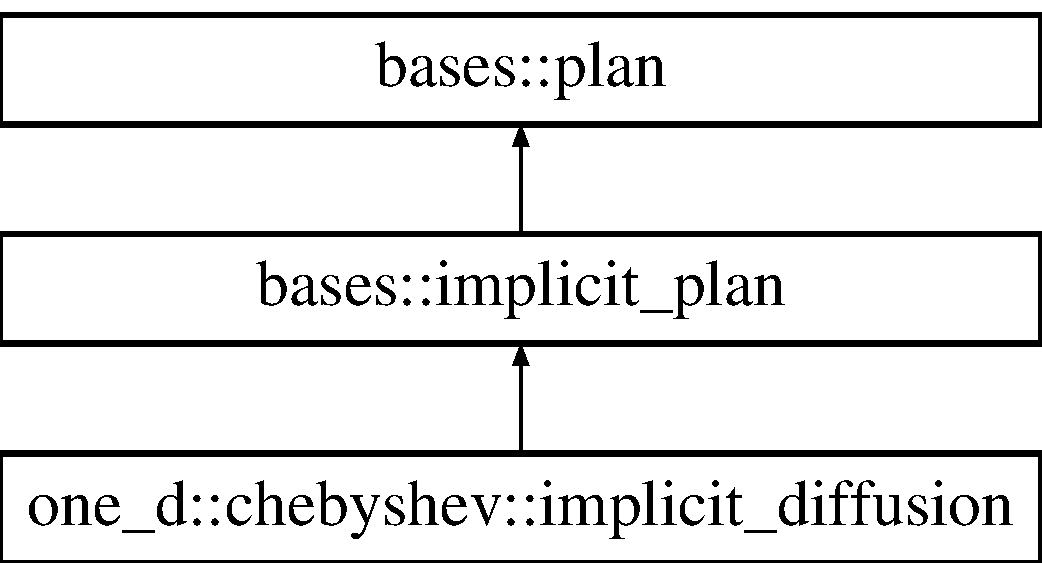
\includegraphics[height=3.000000cm]{classbases_1_1implicit__plan}
\end{center}
\end{figure}
\subsection*{Public Member Functions}
\begin{DoxyCompactItemize}
\item 
\hyperlink{classbases_1_1implicit__plan_aee12711a50c3fdec6da0861fba6736f1}{implicit\-\_\-plan} (\hyperlink{classbases_1_1element}{element} $\ast$i\-\_\-element\-\_\-ptr, int i\-\_\-n, \hyperlink{classbases_1_1collocation__grid}{bases\-::collocation\-\_\-grid} $\ast$i\-\_\-grid, double $\ast$i\-\_\-matrix, int i\-\_\-flags=0x00)
\begin{DoxyCompactList}\small\item\em \end{DoxyCompactList}\item 
virtual void \hyperlink{classbases_1_1implicit__plan_a564bcb2be88ca9abe77c981d77d58d74}{execute} ()
\begin{DoxyCompactList}\small\item\em Operate the plan on the data arrays contained in the class. \end{DoxyCompactList}\end{DoxyCompactItemize}
\subsection*{Protected Attributes}
\begin{DoxyCompactItemize}
\item 
\hypertarget{classbases_1_1implicit__plan_a43fa2adfff9e68a66a23cf03b027a32d}{int \hyperlink{classbases_1_1implicit__plan_a43fa2adfff9e68a66a23cf03b027a32d}{n}}\label{classbases_1_1implicit__plan_a43fa2adfff9e68a66a23cf03b027a32d}

\begin{DoxyCompactList}\small\item\em An integer number of data elements. \end{DoxyCompactList}\item 
\hypertarget{classbases_1_1implicit__plan_a23a0aa32f42b2ba03ef47ba60567522b}{\hyperlink{classbases_1_1collocation__grid}{bases\-::collocation\-\_\-grid} $\ast$ \hyperlink{classbases_1_1implicit__plan_a23a0aa32f42b2ba03ef47ba60567522b}{grid}}\label{classbases_1_1implicit__plan_a23a0aa32f42b2ba03ef47ba60567522b}

\begin{DoxyCompactList}\small\item\em A shared pointer to the grid. \end{DoxyCompactList}\item 
\hypertarget{classbases_1_1implicit__plan_af9d3db062039649e63a7fe1f83a9d155}{double $\ast$ \hyperlink{classbases_1_1implicit__plan_af9d3db062039649e63a7fe1f83a9d155}{matrix}}\label{classbases_1_1implicit__plan_af9d3db062039649e63a7fe1f83a9d155}

\begin{DoxyCompactList}\small\item\em A double pointer to the input data. \end{DoxyCompactList}\end{DoxyCompactItemize}


\subsection{Detailed Description}
A subclass of plan, specific to implicit methods. 



 These plans produce output in a square matrix but take no input. 

\subsection{Constructor \& Destructor Documentation}
\hypertarget{classbases_1_1implicit__plan_aee12711a50c3fdec6da0861fba6736f1}{\index{bases\-::implicit\-\_\-plan@{bases\-::implicit\-\_\-plan}!implicit\-\_\-plan@{implicit\-\_\-plan}}
\index{implicit\-\_\-plan@{implicit\-\_\-plan}!bases::implicit_plan@{bases\-::implicit\-\_\-plan}}
\subsubsection[{implicit\-\_\-plan}]{\setlength{\rightskip}{0pt plus 5cm}bases\-::implicit\-\_\-plan\-::implicit\-\_\-plan (
\begin{DoxyParamCaption}
\item[{{\bf element} $\ast$}]{i\-\_\-element\-\_\-ptr, }
\item[{int}]{i\-\_\-n, }
\item[{{\bf bases\-::collocation\-\_\-grid} $\ast$}]{i\-\_\-grid, }
\item[{double $\ast$}]{i\-\_\-matrix, }
\item[{int}]{i\-\_\-flags = {\ttfamily 0x00}}
\end{DoxyParamCaption}
)\hspace{0.3cm}{\ttfamily [inline]}}}\label{classbases_1_1implicit__plan_aee12711a50c3fdec6da0861fba6736f1}






 
\begin{DoxyParams}{Parameters}
{\em i\-\_\-n} & The integer number of elements in a row of the square i\-\_\-matrix \\
\hline
{\em i\-\_\-grid} & A shared pointer to the collocation grid object \\
\hline
{\em i\-\_\-matrix} & The double matrix to be updated \\
\hline
\end{DoxyParams}


 
\begin{DoxyParams}{Parameters}
{\em i\-\_\-element\-\_\-ptr} & A pointer to the associated element \\
\hline
\end{DoxyParams}


\subsection{Member Function Documentation}
\hypertarget{classbases_1_1implicit__plan_a564bcb2be88ca9abe77c981d77d58d74}{\index{bases\-::implicit\-\_\-plan@{bases\-::implicit\-\_\-plan}!execute@{execute}}
\index{execute@{execute}!bases::implicit_plan@{bases\-::implicit\-\_\-plan}}
\subsubsection[{execute}]{\setlength{\rightskip}{0pt plus 5cm}void bases\-::implicit\-\_\-plan\-::execute (
\begin{DoxyParamCaption}
{}
\end{DoxyParamCaption}
)\hspace{0.3cm}{\ttfamily [virtual]}}}\label{classbases_1_1implicit__plan_a564bcb2be88ca9abe77c981d77d58d74}


Operate the plan on the data arrays contained in the class. 



 

 The plan class serves as a wrapper for this function. 

Reimplemented from \hyperlink{classbases_1_1plan_a85d7e7f7a04ac8213ea57bde32db34c2}{bases\-::plan}.



Reimplemented in \hyperlink{classone__d_1_1chebyshev_1_1implicit__diffusion_a5da5289b943a5d3384c7b0341f890125}{one\-\_\-d\-::chebyshev\-::implicit\-\_\-diffusion}.



The documentation for this class was generated from the following files\-:\begin{DoxyCompactItemize}
\item 
/\-Users/justinbrown/\-Dropbox/spectral\-\_\-element/src/bases/\hyperlink{plan_8hpp}{plan.\-hpp}\item 
/\-Users/justinbrown/\-Dropbox/spectral\-\_\-element/src/bases/\hyperlink{plan_8cpp}{plan.\-cpp}\end{DoxyCompactItemize}

\hypertarget{classio_1_1incremental__output}{\section{io\-:\-:incremental\-\_\-output Class Reference}
\label{classio_1_1incremental__output}\index{io\-::incremental\-\_\-output@{io\-::incremental\-\_\-output}}
}


An incremental implementation of the output class.  




{\ttfamily \#include $<$io.\-hpp$>$}

Inheritance diagram for io\-:\-:incremental\-\_\-output\-:\begin{figure}[H]
\begin{center}
\leavevmode
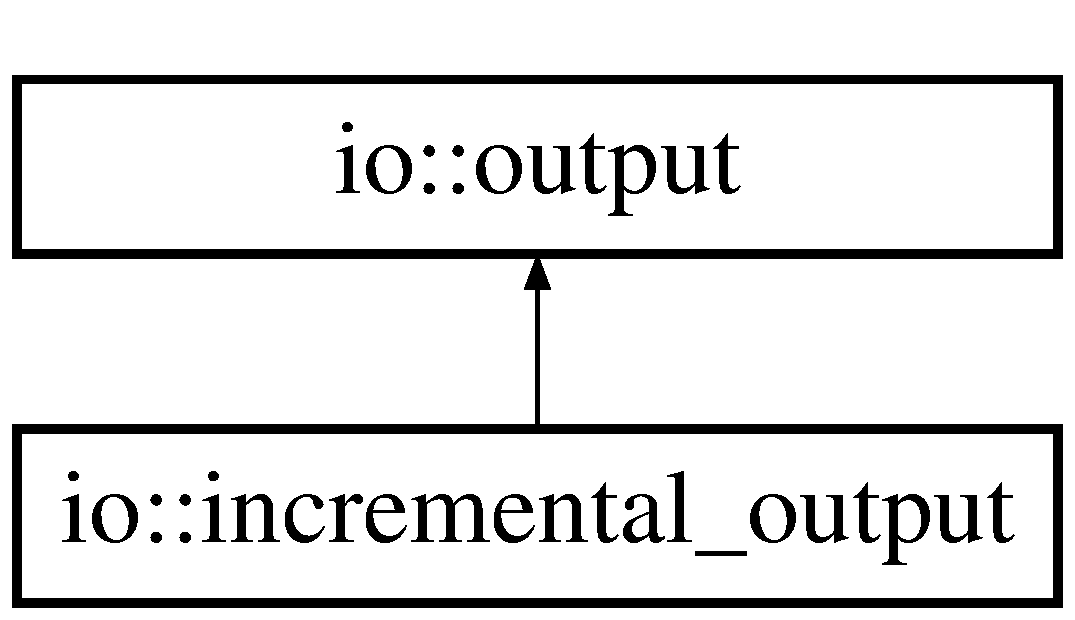
\includegraphics[height=2.000000cm]{classio_1_1incremental__output}
\end{center}
\end{figure}
\subsection*{Public Member Functions}
\begin{DoxyCompactItemize}
\item 
\hyperlink{classio_1_1incremental__output_a01308d0fb0a638bd9f382deecfbe82a5}{incremental\-\_\-output} (std\-::string i\-\_\-file\-\_\-base, std\-::string i\-\_\-file\-\_\-extension, int i\-\_\-int\-\_\-width, \hyperlink{classio_1_1header}{header} $\ast$i\-\_\-header\-\_\-ptr, int i\-\_\-n, int i\-\_\-output\-\_\-every)
\item 
std\-::string \hyperlink{classio_1_1incremental__output_a239bbe0e73c9c26b7eab7970dac95a56}{generate\-\_\-file\-\_\-name} ()
\begin{DoxyCompactList}\small\item\em Generates the next file name in the sequence. \end{DoxyCompactList}\item 
void \hyperlink{classio_1_1incremental__output_a966b0a04f3150e1060d69fd08aed0c99}{to\-\_\-file} ()
\begin{DoxyCompactList}\small\item\em Outputs to file. \end{DoxyCompactList}\end{DoxyCompactItemize}
\subsection*{Additional Inherited Members}


\subsection{Detailed Description}
An incremental implementation of the output class. 



 This class is an implementation of the output class that increments the file number with each iteration. 

\subsection{Constructor \& Destructor Documentation}
\hypertarget{classio_1_1incremental__output_a01308d0fb0a638bd9f382deecfbe82a5}{\index{io\-::incremental\-\_\-output@{io\-::incremental\-\_\-output}!incremental\-\_\-output@{incremental\-\_\-output}}
\index{incremental\-\_\-output@{incremental\-\_\-output}!io::incremental_output@{io\-::incremental\-\_\-output}}
\subsubsection[{incremental\-\_\-output}]{\setlength{\rightskip}{0pt plus 5cm}io\-::incremental\-\_\-output\-::incremental\-\_\-output (
\begin{DoxyParamCaption}
\item[{std\-::string}]{i\-\_\-file\-\_\-base, }
\item[{std\-::string}]{i\-\_\-file\-\_\-extension, }
\item[{int}]{i\-\_\-int\-\_\-width, }
\item[{{\bf header} $\ast$}]{i\-\_\-header\-\_\-ptr, }
\item[{int}]{i\-\_\-n, }
\item[{int}]{i\-\_\-output\-\_\-every}
\end{DoxyParamCaption}
)\hspace{0.3cm}{\ttfamily [inline]}}}\label{classio_1_1incremental__output_a01308d0fb0a638bd9f382deecfbe82a5}


 
\begin{DoxyParams}{Parameters}
{\em i\-\_\-file\-\_\-base} & A string containing the file name base (the string before the numbers, including the path) \\
\hline
{\em i\-\_\-file\-\_\-extension} & A string containing the file name extension (the string after the numbers, including the '.') \\
\hline
{\em i\-\_\-int\-\_\-width} & The total number of characters the integer in the file name can have \\
\hline
{\em i\-\_\-header\-\_\-ptr} & A pointer to the header object \\
\hline
{\em i\-\_\-n} & The integer number of points in the data \\
\hline
{\em i\-\_\-output\-\_\-every} & An integer number of steps between outputs \\
\hline
\end{DoxyParams}


\subsection{Member Function Documentation}
\hypertarget{classio_1_1incremental__output_a239bbe0e73c9c26b7eab7970dac95a56}{\index{io\-::incremental\-\_\-output@{io\-::incremental\-\_\-output}!generate\-\_\-file\-\_\-name@{generate\-\_\-file\-\_\-name}}
\index{generate\-\_\-file\-\_\-name@{generate\-\_\-file\-\_\-name}!io::incremental_output@{io\-::incremental\-\_\-output}}
\subsubsection[{generate\-\_\-file\-\_\-name}]{\setlength{\rightskip}{0pt plus 5cm}std\-::string io\-::incremental\-\_\-output\-::generate\-\_\-file\-\_\-name (
\begin{DoxyParamCaption}
{}
\end{DoxyParamCaption}
)}}\label{classio_1_1incremental__output_a239bbe0e73c9c26b7eab7970dac95a56}


Generates the next file name in the sequence. 



 \begin{DoxyReturn}{Returns}
The incremented file name 
\end{DoxyReturn}
\hypertarget{classio_1_1incremental__output_a966b0a04f3150e1060d69fd08aed0c99}{\index{io\-::incremental\-\_\-output@{io\-::incremental\-\_\-output}!to\-\_\-file@{to\-\_\-file}}
\index{to\-\_\-file@{to\-\_\-file}!io::incremental_output@{io\-::incremental\-\_\-output}}
\subsubsection[{to\-\_\-file}]{\setlength{\rightskip}{0pt plus 5cm}void io\-::incremental\-\_\-output\-::to\-\_\-file (
\begin{DoxyParamCaption}
{}
\end{DoxyParamCaption}
)\hspace{0.3cm}{\ttfamily [inline]}, {\ttfamily [virtual]}}}\label{classio_1_1incremental__output_a966b0a04f3150e1060d69fd08aed0c99}


Outputs to file. 



 

Implements \hyperlink{classio_1_1output_aae295dd37ca6397fcf8c2109f2c0e418}{io\-::output}.



The documentation for this class was generated from the following files\-:\begin{DoxyCompactItemize}
\item 
/\-Users/justinbrown/\-Dropbox/spectral\-\_\-element/src/utils/\hyperlink{io_8hpp}{io.\-hpp}\item 
/\-Users/justinbrown/\-Dropbox/spectral\-\_\-element/src/utils/\hyperlink{io_8cpp}{io.\-cpp}\end{DoxyCompactItemize}

\hypertarget{classlog__config}{\section{log\-\_\-config Class Reference}
\label{classlog__config}\index{log\-\_\-config@{log\-\_\-config}}
}


A class containing the relevant configuration details, such as logging severity.  




{\ttfamily \#include $<$config.\-hpp$>$}

\subsection*{Static Public Member Functions}
\begin{DoxyCompactItemize}
\item 
static void \hyperlink{classlog__config_a00103c7e762a66cb5e7717f3dfb46c53}{update\-\_\-severity} (int severity\-\_\-index)
\begin{DoxyCompactList}\small\item\em Updates the severity of the logger. \end{DoxyCompactList}\item 
static void \hyperlink{classlog__config_ae9fa43978bbf0007ff911eed5b46d17c}{update\-\_\-name} (int id)
\begin{DoxyCompactList}\small\item\em Updates the name of the logger and log file. \end{DoxyCompactList}\end{DoxyCompactItemize}
\subsection*{Static Public Attributes}
\begin{DoxyCompactItemize}
\item 
\hypertarget{classlog__config_a834f2cce03a7594e4f112d21ff72d260}{static int \hyperlink{classlog__config_a834f2cce03a7594e4f112d21ff72d260}{severity} = 2}\label{classlog__config_a834f2cce03a7594e4f112d21ff72d260}

\begin{DoxyCompactList}\small\item\em The integer level of severity to be output in the log. \end{DoxyCompactList}\end{DoxyCompactItemize}


\subsection{Detailed Description}
A class containing the relevant configuration details, such as logging severity. 



 

\subsection{Member Function Documentation}
\hypertarget{classlog__config_ae9fa43978bbf0007ff911eed5b46d17c}{\index{log\-\_\-config@{log\-\_\-config}!update\-\_\-name@{update\-\_\-name}}
\index{update\-\_\-name@{update\-\_\-name}!log_config@{log\-\_\-config}}
\subsubsection[{update\-\_\-name}]{\setlength{\rightskip}{0pt plus 5cm}void log\-\_\-config\-::update\-\_\-name (
\begin{DoxyParamCaption}
\item[{int}]{id}
\end{DoxyParamCaption}
)\hspace{0.3cm}{\ttfamily [static]}}}\label{classlog__config_ae9fa43978bbf0007ff911eed5b46d17c}


Updates the name of the logger and log file. 



 The name of the logger becomes element\-\_\-id, and the file name element\-\_\-id.\-log.


\begin{DoxyParams}{Parameters}
{\em id} & The integer id with which to label the log. \\
\hline
\end{DoxyParams}
\hypertarget{classlog__config_a00103c7e762a66cb5e7717f3dfb46c53}{\index{log\-\_\-config@{log\-\_\-config}!update\-\_\-severity@{update\-\_\-severity}}
\index{update\-\_\-severity@{update\-\_\-severity}!log_config@{log\-\_\-config}}
\subsubsection[{update\-\_\-severity}]{\setlength{\rightskip}{0pt plus 5cm}void log\-\_\-config\-::update\-\_\-severity (
\begin{DoxyParamCaption}
\item[{int}]{severity\-\_\-index}
\end{DoxyParamCaption}
)\hspace{0.3cm}{\ttfamily [static]}}}\label{classlog__config_a00103c7e762a66cb5e7717f3dfb46c53}


Updates the severity of the logger. 



 The severity scheme is as follows\-: 0\-: Trace\-: Indicates a code location, used for optimization 1\-: Debug\-: Used to diagnose bugs 2\-: Info\-: Produces relevant information to user (default) 3\-: Warn\-: May indicate an issue, depending on user intent 4\-: Error\-: A problem that can be handled has occurred 5\-: Fatal\-: A problem that cannot be handled has occurred


\begin{DoxyParams}{Parameters}
{\em severity\-\_\-index} & The integer severity below which log statements are suppressed \\
\hline
\end{DoxyParams}


The documentation for this class was generated from the following files\-:\begin{DoxyCompactItemize}
\item 
/\-Users/justinbrown/\-Dropbox/spectral\-\_\-element/src/\hyperlink{config_8hpp}{config.\-hpp}\item 
/\-Users/justinbrown/\-Dropbox/spectral\-\_\-element/src/\hyperlink{config_8cpp}{config.\-cpp}\end{DoxyCompactItemize}

\hypertarget{classbases_1_1messenger}{\section{bases\-:\-:messenger Class Reference}
\label{classbases_1_1messenger}\index{bases\-::messenger@{bases\-::messenger}}
}


A class to manage boundary communication.  




{\ttfamily \#include $<$messenger.\-hpp$>$}

\subsection*{Public Member Functions}
\begin{DoxyCompactItemize}
\item 
\hyperlink{classbases_1_1messenger_ae4aade26c6ef7809a30659471a6d0ad2}{messenger} (int $\ast$argc, char $\ast$$\ast$$\ast$argv, int n\-\_\-boundaries)
\item 
int \hyperlink{classbases_1_1messenger_a6aa3309dfbebace3cec88f57cf9edfce}{get\-\_\-id} ()
\begin{DoxyCompactList}\small\item\em Return the id of the current process. \end{DoxyCompactList}\item 
int \hyperlink{classbases_1_1messenger_ad5eda2bab3d38ae383579108a03f2c5b}{get\-\_\-np} ()
\begin{DoxyCompactList}\small\item\em Return the total number of processes. \end{DoxyCompactList}\item 
bool \hyperlink{classbases_1_1messenger_ae7e221a16bc75c302fe3d48a63359be7}{linked} (int edge)
\begin{DoxyCompactList}\small\item\em Return whether the specified edge is linked. \end{DoxyCompactList}\item 
virtual int \hyperlink{classbases_1_1messenger_a7d9b96f1b04598c480d367a95015cc72}{edge\-\_\-to\-\_\-index} (int mode, int edge)
\begin{DoxyCompactList}\small\item\em Given an edge and action mode, determine the correct index. \end{DoxyCompactList}\item 
virtual int \hyperlink{classbases_1_1messenger_a419d764733431f850130f1024fbe75fc}{index\-\_\-to\-\_\-mode} (int \hyperlink{plan_8hpp_a6784e1c334dfceb8f017667c0b0f6a3e}{index})
\begin{DoxyCompactList}\small\item\em Given an index, determine whether to send or recv. \end{DoxyCompactList}\item 
virtual void \hyperlink{classbases_1_1messenger_a64687bc91d7e8c818951eb311ec59bb8}{add\-\_\-boundary} (int edge, int process)
\begin{DoxyCompactList}\small\item\em Link this element with another. \end{DoxyCompactList}\item 
virtual void \hyperlink{classbases_1_1messenger_ad0d6143a787a00261784493ec7413a17}{send} (int n, double $\ast$data, int edge)
\begin{DoxyCompactList}\small\item\em Add send action in the double queue. \end{DoxyCompactList}\item 
virtual void \hyperlink{classbases_1_1messenger_a5d43e922b30cbe13f76f3ff46511601b}{recv} (int n, double $\ast$data, int edge)
\begin{DoxyCompactList}\small\item\em Add recv action in the double queue. \end{DoxyCompactList}\item 
virtual void \hyperlink{classbases_1_1messenger_a7a0b0da172ae2a53693e330daf945acf}{send} (int n, int $\ast$data, int edge)
\begin{DoxyCompactList}\small\item\em Add send action in the integer queue. \end{DoxyCompactList}\item 
virtual void \hyperlink{classbases_1_1messenger_ae59f0a20772afbb06c836310b3a3f452}{recv} (int n, int $\ast$data, int edge)
\begin{DoxyCompactList}\small\item\em Add recv action in the integer queue. \end{DoxyCompactList}\item 
virtual void \hyperlink{classbases_1_1messenger_a7d14d988ce500b9c56a34b44b6e6ca94}{min} (double $\ast$data)
\begin{DoxyCompactList}\small\item\em Calculate a minimum across elements. \end{DoxyCompactList}\item 
virtual bool \hyperlink{classbases_1_1messenger_a9f711b71b09ca9940a7363c821307c93}{bool\-\_\-and} (bool boolean)
\begin{DoxyCompactList}\small\item\em Determine if all processes meet a condition. \end{DoxyCompactList}\end{DoxyCompactItemize}


\subsection{Detailed Description}
A class to manage boundary communication. 



 This class should provide implementation to send boundary information to other elements. It may be dimension specific. There should only be one per thread. 

\subsection{Constructor \& Destructor Documentation}
\hypertarget{classbases_1_1messenger_ae4aade26c6ef7809a30659471a6d0ad2}{\index{bases\-::messenger@{bases\-::messenger}!messenger@{messenger}}
\index{messenger@{messenger}!bases::messenger@{bases\-::messenger}}
\subsubsection[{messenger}]{\setlength{\rightskip}{0pt plus 5cm}bases\-::messenger\-::messenger (
\begin{DoxyParamCaption}
\item[{int $\ast$}]{argc, }
\item[{char $\ast$$\ast$$\ast$}]{argv, }
\item[{int}]{n\-\_\-boundaries}
\end{DoxyParamCaption}
)}}\label{classbases_1_1messenger_ae4aade26c6ef7809a30659471a6d0ad2}


 
\begin{DoxyParams}{Parameters}
{\em argc} & An integer pointer to the number of command arguments \\
\hline
{\em argv} & A pointer to an array of character arrays of command arguments \\
\hline
{\em n\-\_\-boundaries} & The integer number of boundaries per element (must be even) \\
\hline
\end{DoxyParams}


\subsection{Member Function Documentation}
\hypertarget{classbases_1_1messenger_a64687bc91d7e8c818951eb311ec59bb8}{\index{bases\-::messenger@{bases\-::messenger}!add\-\_\-boundary@{add\-\_\-boundary}}
\index{add\-\_\-boundary@{add\-\_\-boundary}!bases::messenger@{bases\-::messenger}}
\subsubsection[{add\-\_\-boundary}]{\setlength{\rightskip}{0pt plus 5cm}void bases\-::messenger\-::add\-\_\-boundary (
\begin{DoxyParamCaption}
\item[{int}]{edge, }
\item[{int}]{process}
\end{DoxyParamCaption}
)\hspace{0.3cm}{\ttfamily [virtual]}}}\label{classbases_1_1messenger_a64687bc91d7e8c818951eb311ec59bb8}


Link this element with another. 



 
\begin{DoxyParams}{Parameters}
{\em edge} & The integer representation of the edge to link \\
\hline
{\em process} & The integer id of the process to link to \\
\hline
\end{DoxyParams}
\hypertarget{classbases_1_1messenger_a9f711b71b09ca9940a7363c821307c93}{\index{bases\-::messenger@{bases\-::messenger}!bool\-\_\-and@{bool\-\_\-and}}
\index{bool\-\_\-and@{bool\-\_\-and}!bases::messenger@{bases\-::messenger}}
\subsubsection[{bool\-\_\-and}]{\setlength{\rightskip}{0pt plus 5cm}bool bases\-::messenger\-::bool\-\_\-and (
\begin{DoxyParamCaption}
\item[{bool}]{boolean}
\end{DoxyParamCaption}
)\hspace{0.3cm}{\ttfamily [virtual]}}}\label{classbases_1_1messenger_a9f711b71b09ca9940a7363c821307c93}


Determine if all processes meet a condition. 



 This uses the messenger integer buffer.


\begin{DoxyParams}{Parameters}
{\em boolean} & The bool condition to check \\
\hline
\end{DoxyParams}
\hypertarget{classbases_1_1messenger_a7d9b96f1b04598c480d367a95015cc72}{\index{bases\-::messenger@{bases\-::messenger}!edge\-\_\-to\-\_\-index@{edge\-\_\-to\-\_\-index}}
\index{edge\-\_\-to\-\_\-index@{edge\-\_\-to\-\_\-index}!bases::messenger@{bases\-::messenger}}
\subsubsection[{edge\-\_\-to\-\_\-index}]{\setlength{\rightskip}{0pt plus 5cm}virtual int bases\-::messenger\-::edge\-\_\-to\-\_\-index (
\begin{DoxyParamCaption}
\item[{int}]{mode, }
\item[{int}]{edge}
\end{DoxyParamCaption}
)\hspace{0.3cm}{\ttfamily [inline]}, {\ttfamily [virtual]}}}\label{classbases_1_1messenger_a7d9b96f1b04598c480d367a95015cc72}


Given an edge and action mode, determine the correct index. 



 Each action on each edge has a queue index, which this function reads


\begin{DoxyParams}{Parameters}
{\em mode} & The integer representation of the action (0 for send, 1 for recv) \\
\hline
{\em edge} & The integer representation of the edge \\
\hline
\end{DoxyParams}
\hypertarget{classbases_1_1messenger_a6aa3309dfbebace3cec88f57cf9edfce}{\index{bases\-::messenger@{bases\-::messenger}!get\-\_\-id@{get\-\_\-id}}
\index{get\-\_\-id@{get\-\_\-id}!bases::messenger@{bases\-::messenger}}
\subsubsection[{get\-\_\-id}]{\setlength{\rightskip}{0pt plus 5cm}int bases\-::messenger\-::get\-\_\-id (
\begin{DoxyParamCaption}
{}
\end{DoxyParamCaption}
)\hspace{0.3cm}{\ttfamily [inline]}}}\label{classbases_1_1messenger_a6aa3309dfbebace3cec88f57cf9edfce}


Return the id of the current process. 



 \begin{DoxyReturn}{Returns}
The integer id of the current process 
\end{DoxyReturn}
\hypertarget{classbases_1_1messenger_ad5eda2bab3d38ae383579108a03f2c5b}{\index{bases\-::messenger@{bases\-::messenger}!get\-\_\-np@{get\-\_\-np}}
\index{get\-\_\-np@{get\-\_\-np}!bases::messenger@{bases\-::messenger}}
\subsubsection[{get\-\_\-np}]{\setlength{\rightskip}{0pt plus 5cm}int bases\-::messenger\-::get\-\_\-np (
\begin{DoxyParamCaption}
{}
\end{DoxyParamCaption}
)\hspace{0.3cm}{\ttfamily [inline]}}}\label{classbases_1_1messenger_ad5eda2bab3d38ae383579108a03f2c5b}


Return the total number of processes. 



 \begin{DoxyReturn}{Returns}
The integer number of processes 
\end{DoxyReturn}
\hypertarget{classbases_1_1messenger_a419d764733431f850130f1024fbe75fc}{\index{bases\-::messenger@{bases\-::messenger}!index\-\_\-to\-\_\-mode@{index\-\_\-to\-\_\-mode}}
\index{index\-\_\-to\-\_\-mode@{index\-\_\-to\-\_\-mode}!bases::messenger@{bases\-::messenger}}
\subsubsection[{index\-\_\-to\-\_\-mode}]{\setlength{\rightskip}{0pt plus 5cm}virtual int bases\-::messenger\-::index\-\_\-to\-\_\-mode (
\begin{DoxyParamCaption}
\item[{int}]{index}
\end{DoxyParamCaption}
)\hspace{0.3cm}{\ttfamily [inline]}, {\ttfamily [virtual]}}}\label{classbases_1_1messenger_a419d764733431f850130f1024fbe75fc}


Given an index, determine whether to send or recv. 



 
\begin{DoxyParams}{Parameters}
{\em index} & The queue index of the action \\
\hline
\end{DoxyParams}
\hypertarget{classbases_1_1messenger_ae7e221a16bc75c302fe3d48a63359be7}{\index{bases\-::messenger@{bases\-::messenger}!linked@{linked}}
\index{linked@{linked}!bases::messenger@{bases\-::messenger}}
\subsubsection[{linked}]{\setlength{\rightskip}{0pt plus 5cm}bool bases\-::messenger\-::linked (
\begin{DoxyParamCaption}
\item[{int}]{edge}
\end{DoxyParamCaption}
)\hspace{0.3cm}{\ttfamily [inline]}}}\label{classbases_1_1messenger_ae7e221a16bc75c302fe3d48a63359be7}


Return whether the specified edge is linked. 



 \begin{DoxyReturn}{Returns}
A bool of if the edge is linked to another process 
\end{DoxyReturn}
\hypertarget{classbases_1_1messenger_a7d14d988ce500b9c56a34b44b6e6ca94}{\index{bases\-::messenger@{bases\-::messenger}!min@{min}}
\index{min@{min}!bases::messenger@{bases\-::messenger}}
\subsubsection[{min}]{\setlength{\rightskip}{0pt plus 5cm}void bases\-::messenger\-::min (
\begin{DoxyParamCaption}
\item[{double $\ast$}]{data}
\end{DoxyParamCaption}
)\hspace{0.3cm}{\ttfamily [virtual]}}}\label{classbases_1_1messenger_a7d14d988ce500b9c56a34b44b6e6ca94}


Calculate a minimum across elements. 



 This uses the messenger buffer.


\begin{DoxyParams}{Parameters}
{\em data} & The double pointer to the double to minimize \\
\hline
\end{DoxyParams}
\hypertarget{classbases_1_1messenger_a5d43e922b30cbe13f76f3ff46511601b}{\index{bases\-::messenger@{bases\-::messenger}!recv@{recv}}
\index{recv@{recv}!bases::messenger@{bases\-::messenger}}
\subsubsection[{recv}]{\setlength{\rightskip}{0pt plus 5cm}void bases\-::messenger\-::recv (
\begin{DoxyParamCaption}
\item[{int}]{n, }
\item[{double $\ast$}]{data, }
\item[{int}]{edge}
\end{DoxyParamCaption}
)\hspace{0.3cm}{\ttfamily [virtual]}}}\label{classbases_1_1messenger_a5d43e922b30cbe13f76f3ff46511601b}


Add recv action in the double queue. 



 Warning. This does not recv the data immediately. This could be rewritten to wait for the information, but it does not at present. It recvs if it can, but the information is not guaranteed to arrive until an entire set of send/recv commands are queued.


\begin{DoxyParams}{Parameters}
{\em n} & The integer number of elements to recv \\
\hline
{\em data} & The double pointer to the data to recv \\
\hline
{\em edge} & The integer representation of the corresponding edge \\
\hline
\end{DoxyParams}
\hypertarget{classbases_1_1messenger_ae59f0a20772afbb06c836310b3a3f452}{\index{bases\-::messenger@{bases\-::messenger}!recv@{recv}}
\index{recv@{recv}!bases::messenger@{bases\-::messenger}}
\subsubsection[{recv}]{\setlength{\rightskip}{0pt plus 5cm}void bases\-::messenger\-::recv (
\begin{DoxyParamCaption}
\item[{int}]{n, }
\item[{int $\ast$}]{data, }
\item[{int}]{edge}
\end{DoxyParamCaption}
)\hspace{0.3cm}{\ttfamily [virtual]}}}\label{classbases_1_1messenger_ae59f0a20772afbb06c836310b3a3f452}


Add recv action in the integer queue. 



 Warning. This does not recv the data immediately. This could be rewritten to wait for the information, but it does not at present. It recvs if it can, but the information is not guaranteed to arrive until an entire set of send/recv commands are queued.


\begin{DoxyParams}{Parameters}
{\em n} & The integer number of elements to recv \\
\hline
{\em data} & The integer pointer to the data to recv \\
\hline
{\em edge} & The integer representation of the corresponding edge \\
\hline
\end{DoxyParams}
\hypertarget{classbases_1_1messenger_ad0d6143a787a00261784493ec7413a17}{\index{bases\-::messenger@{bases\-::messenger}!send@{send}}
\index{send@{send}!bases::messenger@{bases\-::messenger}}
\subsubsection[{send}]{\setlength{\rightskip}{0pt plus 5cm}void bases\-::messenger\-::send (
\begin{DoxyParamCaption}
\item[{int}]{n, }
\item[{double $\ast$}]{data, }
\item[{int}]{edge}
\end{DoxyParamCaption}
)\hspace{0.3cm}{\ttfamily [virtual]}}}\label{classbases_1_1messenger_ad0d6143a787a00261784493ec7413a17}


Add send action in the double queue. 



 Warning. This does not send the data immediately. This could be rewritten to save the information in a buffer, but it does not at present. It sends if it can, but the information is not guaranteed to be sent until an entire set of send/recv commands are queued.


\begin{DoxyParams}{Parameters}
{\em n} & The integer number of elements to send \\
\hline
{\em data} & The double pointer to the data to send \\
\hline
{\em edge} & The integer representation of the corresponding edge \\
\hline
\end{DoxyParams}
\hypertarget{classbases_1_1messenger_a7a0b0da172ae2a53693e330daf945acf}{\index{bases\-::messenger@{bases\-::messenger}!send@{send}}
\index{send@{send}!bases::messenger@{bases\-::messenger}}
\subsubsection[{send}]{\setlength{\rightskip}{0pt plus 5cm}void bases\-::messenger\-::send (
\begin{DoxyParamCaption}
\item[{int}]{n, }
\item[{int $\ast$}]{data, }
\item[{int}]{edge}
\end{DoxyParamCaption}
)\hspace{0.3cm}{\ttfamily [virtual]}}}\label{classbases_1_1messenger_a7a0b0da172ae2a53693e330daf945acf}


Add send action in the integer queue. 



 Warning. This does not send the data immediately. This could be rewritten to save the information in a buffer, but it does not at present. It sends if it can, but the information is not guaranteed to be sent until an entire set of send/recv commands are queued.


\begin{DoxyParams}{Parameters}
{\em n} & The integer number of elements to send \\
\hline
{\em data} & The integer pointer to the data to send \\
\hline
{\em edge} & The integer representation of the corresponding edge \\
\hline
\end{DoxyParams}


The documentation for this class was generated from the following files\-:\begin{DoxyCompactItemize}
\item 
/\-Users/justinbrown/\-Dropbox/spectral\-\_\-element/src/bases/\hyperlink{messenger_8hpp}{messenger.\-hpp}\item 
/\-Users/justinbrown/\-Dropbox/spectral\-\_\-element/src/bases/\hyperlink{messenger_8cpp}{messenger.\-cpp}\end{DoxyCompactItemize}

\hypertarget{classio_1_1output}{\section{io\-:\-:output Class Reference}
\label{classio_1_1output}\index{io\-::output@{io\-::output}}
}


An abstract output stream base class that generates output files.  




{\ttfamily \#include $<$io.\-hpp$>$}

Inheritance diagram for io\-:\-:output\-:\begin{figure}[H]
\begin{center}
\leavevmode
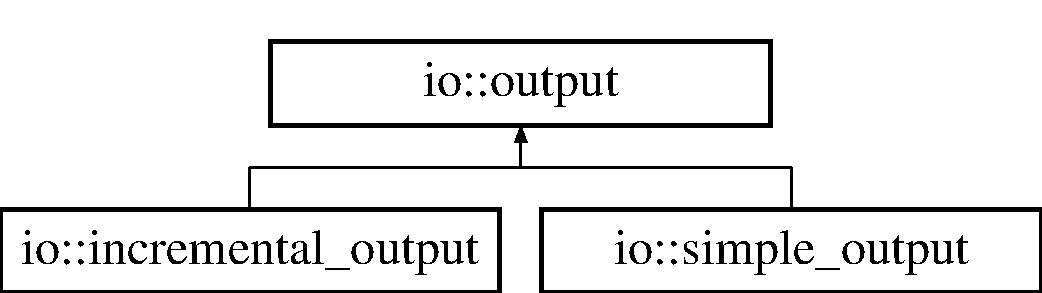
\includegraphics[height=2.000000cm]{classio_1_1output}
\end{center}
\end{figure}
\subsection*{Public Member Functions}
\begin{DoxyCompactItemize}
\item 
\hyperlink{classio_1_1output_af2cf6a328dfae9737484dc52cb804a6e}{output} (\hyperlink{classio_1_1header}{header} $\ast$i\-\_\-header\-\_\-ptr, int i\-\_\-n)
\item 
virtual void \hyperlink{classio_1_1output_a3dc7c5cc8f0d374d41813c5496a04d7b}{append} (double $\ast$data\-\_\-ptr)
\begin{DoxyCompactList}\small\item\em Append a double array to the list to be output. \end{DoxyCompactList}\item 
virtual void \hyperlink{classio_1_1output_ad77598d1587f724cb928429cbf10d4dd}{append} (double \&data\-\_\-ptr)
\begin{DoxyCompactList}\small\item\em Append a double array to the list to be output. \end{DoxyCompactList}\item 
virtual void \hyperlink{classio_1_1output_a206f90ef42584c60efb44276fd2c691d}{append} (int $\ast$data\-\_\-ptr)
\begin{DoxyCompactList}\small\item\em Append an integer array to the list to be output. \end{DoxyCompactList}\item 
virtual void \hyperlink{classio_1_1output_a39a20cad9edf52ed505efe82726adb92}{append} (int \&data\-\_\-ptr)
\begin{DoxyCompactList}\small\item\em Append an integer array to the list to be output. \end{DoxyCompactList}\item 
virtual void \hyperlink{classio_1_1output_aae295dd37ca6397fcf8c2109f2c0e418}{to\-\_\-file} ()=0
\begin{DoxyCompactList}\small\item\em A virtual function to output the data to file. \end{DoxyCompactList}\end{DoxyCompactItemize}
\subsection*{Protected Member Functions}
\begin{DoxyCompactItemize}
\item 
void \hyperlink{classio_1_1output_a99f92e423caae7ceb24f4da88b3572ff}{std\-\_\-to\-\_\-file} (std\-::string file\-\_\-name)
\begin{DoxyCompactList}\small\item\em Write all the tracked data to file using standard C conversions. \end{DoxyCompactList}\end{DoxyCompactItemize}
\subsection*{Protected Attributes}
\begin{DoxyCompactItemize}
\item 
\hypertarget{classio_1_1output_acc0b537649132b91846a89931933554d}{int \hyperlink{classio_1_1output_acc0b537649132b91846a89931933554d}{n}}\label{classio_1_1output_acc0b537649132b91846a89931933554d}

\begin{DoxyCompactList}\small\item\em An integer number of elements in each array. \end{DoxyCompactList}\item 
\hypertarget{classio_1_1output_a3cd5f0fc09271a653568abc8e10de6aa}{int \hyperlink{classio_1_1output_a3cd5f0fc09271a653568abc8e10de6aa}{n\-\_\-data\-\_\-ptrs}}\label{classio_1_1output_a3cd5f0fc09271a653568abc8e10de6aa}

\begin{DoxyCompactList}\small\item\em An integer number of arrays to output. \end{DoxyCompactList}\item 
\hypertarget{classio_1_1output_a88f0aef3b2bc117e94a876435e59ff96}{std\-::vector$<$ double $\ast$ $>$ \hyperlink{classio_1_1output_a88f0aef3b2bc117e94a876435e59ff96}{double\-\_\-ptrs}}\label{classio_1_1output_a88f0aef3b2bc117e94a876435e59ff96}

\begin{DoxyCompactList}\small\item\em A vector of double pointers to the arrays of data (if an element is N\-U\-L\-L, check int\-\_\-ptrs at the same index instead) \end{DoxyCompactList}\item 
\hypertarget{classio_1_1output_adb08e827090160f0457cb5260bb2998a}{std\-::vector$<$ int $\ast$ $>$ \hyperlink{classio_1_1output_adb08e827090160f0457cb5260bb2998a}{int\-\_\-ptrs}}\label{classio_1_1output_adb08e827090160f0457cb5260bb2998a}

\begin{DoxyCompactList}\small\item\em A vector of integer pointers to the arrays of data. \end{DoxyCompactList}\item 
\hypertarget{classio_1_1output_a9b505ce2bcef3ef4d1bd770b2a718aa0}{std\-::shared\-\_\-ptr$<$ \hyperlink{classio_1_1header}{header} $>$ \hyperlink{classio_1_1output_a9b505ce2bcef3ef4d1bd770b2a718aa0}{header\-\_\-ptr}}\label{classio_1_1output_a9b505ce2bcef3ef4d1bd770b2a718aa0}

\begin{DoxyCompactList}\small\item\em A pointer to a header object, which contains the details regarding the construction of the header. \end{DoxyCompactList}\end{DoxyCompactItemize}


\subsection{Detailed Description}
An abstract output stream base class that generates output files. 



 

\subsection{Constructor \& Destructor Documentation}
\hypertarget{classio_1_1output_af2cf6a328dfae9737484dc52cb804a6e}{\index{io\-::output@{io\-::output}!output@{output}}
\index{output@{output}!io::output@{io\-::output}}
\subsubsection[{output}]{\setlength{\rightskip}{0pt plus 5cm}io\-::output\-::output (
\begin{DoxyParamCaption}
\item[{{\bf header} $\ast$}]{i\-\_\-header\-\_\-ptr, }
\item[{int}]{i\-\_\-n}
\end{DoxyParamCaption}
)}}\label{classio_1_1output_af2cf6a328dfae9737484dc52cb804a6e}


 
\begin{DoxyParams}{Parameters}
{\em i\-\_\-header\-\_\-ptr} & A pointer to the header object \\
\hline
{\em i\-\_\-n} & The integer number of points in the data \\
\hline
\end{DoxyParams}


\subsection{Member Function Documentation}
\hypertarget{classio_1_1output_a3dc7c5cc8f0d374d41813c5496a04d7b}{\index{io\-::output@{io\-::output}!append@{append}}
\index{append@{append}!io::output@{io\-::output}}
\subsubsection[{append}]{\setlength{\rightskip}{0pt plus 5cm}void io\-::output\-::append (
\begin{DoxyParamCaption}
\item[{double $\ast$}]{data\-\_\-ptr}
\end{DoxyParamCaption}
)\hspace{0.3cm}{\ttfamily [virtual]}}}\label{classio_1_1output_a3dc7c5cc8f0d374d41813c5496a04d7b}


Append a double array to the list to be output. 



 
\begin{DoxyParams}{Parameters}
{\em data\-\_\-ptr} & A double pointer to the data to be the new column \\
\hline
\end{DoxyParams}
\hypertarget{classio_1_1output_ad77598d1587f724cb928429cbf10d4dd}{\index{io\-::output@{io\-::output}!append@{append}}
\index{append@{append}!io::output@{io\-::output}}
\subsubsection[{append}]{\setlength{\rightskip}{0pt plus 5cm}virtual void io\-::output\-::append (
\begin{DoxyParamCaption}
\item[{double \&}]{data\-\_\-ptr}
\end{DoxyParamCaption}
)\hspace{0.3cm}{\ttfamily [inline]}, {\ttfamily [virtual]}}}\label{classio_1_1output_ad77598d1587f724cb928429cbf10d4dd}


Append a double array to the list to be output. 



 
\begin{DoxyParams}{Parameters}
{\em data\-\_\-ptr} & A double pointer reference to the data to be the new column \\
\hline
\end{DoxyParams}
\hypertarget{classio_1_1output_a206f90ef42584c60efb44276fd2c691d}{\index{io\-::output@{io\-::output}!append@{append}}
\index{append@{append}!io::output@{io\-::output}}
\subsubsection[{append}]{\setlength{\rightskip}{0pt plus 5cm}void io\-::output\-::append (
\begin{DoxyParamCaption}
\item[{int $\ast$}]{data\-\_\-ptr}
\end{DoxyParamCaption}
)\hspace{0.3cm}{\ttfamily [virtual]}}}\label{classio_1_1output_a206f90ef42584c60efb44276fd2c691d}


Append an integer array to the list to be output. 



 
\begin{DoxyParams}{Parameters}
{\em data\-\_\-ptr} & An integer pointer to the data to be the new column \\
\hline
\end{DoxyParams}
\hypertarget{classio_1_1output_a39a20cad9edf52ed505efe82726adb92}{\index{io\-::output@{io\-::output}!append@{append}}
\index{append@{append}!io::output@{io\-::output}}
\subsubsection[{append}]{\setlength{\rightskip}{0pt plus 5cm}virtual void io\-::output\-::append (
\begin{DoxyParamCaption}
\item[{int \&}]{data\-\_\-ptr}
\end{DoxyParamCaption}
)\hspace{0.3cm}{\ttfamily [inline]}, {\ttfamily [virtual]}}}\label{classio_1_1output_a39a20cad9edf52ed505efe82726adb92}


Append an integer array to the list to be output. 



 
\begin{DoxyParams}{Parameters}
{\em data\-\_\-ptr} & An integer pointer reference to the data to be the new column \\
\hline
\end{DoxyParams}
\hypertarget{classio_1_1output_a99f92e423caae7ceb24f4da88b3572ff}{\index{io\-::output@{io\-::output}!std\-\_\-to\-\_\-file@{std\-\_\-to\-\_\-file}}
\index{std\-\_\-to\-\_\-file@{std\-\_\-to\-\_\-file}!io::output@{io\-::output}}
\subsubsection[{std\-\_\-to\-\_\-file}]{\setlength{\rightskip}{0pt plus 5cm}void io\-::output\-::std\-\_\-to\-\_\-file (
\begin{DoxyParamCaption}
\item[{std\-::string}]{file\-\_\-name}
\end{DoxyParamCaption}
)\hspace{0.3cm}{\ttfamily [protected]}}}\label{classio_1_1output_a99f92e423caae7ceb24f4da88b3572ff}


Write all the tracked data to file using standard C conversions. 



 
\begin{DoxyParams}{Parameters}
{\em file\-\_\-name} & The string name of the file \\
\hline
\end{DoxyParams}
\hypertarget{classio_1_1output_aae295dd37ca6397fcf8c2109f2c0e418}{\index{io\-::output@{io\-::output}!to\-\_\-file@{to\-\_\-file}}
\index{to\-\_\-file@{to\-\_\-file}!io::output@{io\-::output}}
\subsubsection[{to\-\_\-file}]{\setlength{\rightskip}{0pt plus 5cm}virtual void io\-::output\-::to\-\_\-file (
\begin{DoxyParamCaption}
{}
\end{DoxyParamCaption}
)\hspace{0.3cm}{\ttfamily [pure virtual]}}}\label{classio_1_1output_aae295dd37ca6397fcf8c2109f2c0e418}


A virtual function to output the data to file. 



 This function should be overwritten by subclasses, though it may contain a call to this function, which will output with default double representation in C++. 

Implemented in \hyperlink{classio_1_1incremental__output_a966b0a04f3150e1060d69fd08aed0c99}{io\-::incremental\-\_\-output}, and \hyperlink{classio_1_1simple__output_ab0af023314775f6e9e3bf08ee3cc83f9}{io\-::simple\-\_\-output}.



The documentation for this class was generated from the following files\-:\begin{DoxyCompactItemize}
\item 
/\-Users/justinbrown/\-Dropbox/spectral\-\_\-element/src/utils/\hyperlink{io_8hpp}{io.\-hpp}\item 
/\-Users/justinbrown/\-Dropbox/spectral\-\_\-element/src/utils/\hyperlink{io_8cpp}{io.\-cpp}\end{DoxyCompactItemize}

\hypertarget{classbases_1_1plan}{\section{bases\-:\-:plan Class Reference}
\label{classbases_1_1plan}\index{bases\-::plan@{bases\-::plan}}
}


The basic functional unit, containing a recipe for execution.  




{\ttfamily \#include $<$plan.\-hpp$>$}

Inheritance diagram for bases\-:\-:plan\-:\begin{figure}[H]
\begin{center}
\leavevmode
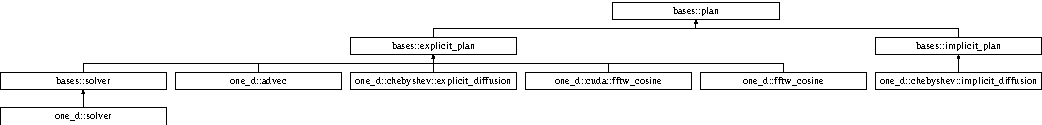
\includegraphics[height=1.674140cm]{classbases_1_1plan}
\end{center}
\end{figure}
\subsection*{Public Member Functions}
\begin{DoxyCompactItemize}
\item 
\hyperlink{classbases_1_1plan_ad0516a1b2b7d3262ea3abab8e8d5edf2}{plan} (\hyperlink{classbases_1_1element}{element} $\ast$i\-\_\-element\-\_\-ptr, int flags=0x00)
\item 
virtual void \hyperlink{classbases_1_1plan_a85d7e7f7a04ac8213ea57bde32db34c2}{execute} ()
\begin{DoxyCompactList}\small\item\em Operate the plan on the data arrays contained in the class. \end{DoxyCompactList}\end{DoxyCompactItemize}
\subsection*{Protected Attributes}
\begin{DoxyCompactItemize}
\item 
\hypertarget{classbases_1_1plan_a54cd8904b8d499e5fc01c8060021d47b}{\hyperlink{classbases_1_1element}{element} $\ast$ \hyperlink{classbases_1_1plan_a54cd8904b8d499e5fc01c8060021d47b}{element\-\_\-ptr}}\label{classbases_1_1plan_a54cd8904b8d499e5fc01c8060021d47b}

\begin{DoxyCompactList}\small\item\em A pointer to the element with which the plan is associated. \end{DoxyCompactList}\item 
\hypertarget{classbases_1_1plan_ad8a2f8000cca7764e9a057c3da1618c4}{int {\bfseries flags}}\label{classbases_1_1plan_ad8a2f8000cca7764e9a057c3da1618c4}

\item 
\hypertarget{classbases_1_1plan_a756595e230cc99e84de4392ac691eefd}{int \hyperlink{classbases_1_1plan_a756595e230cc99e84de4392ac691eefd}{default\-\_\-flags}}\label{classbases_1_1plan_a756595e230cc99e84de4392ac691eefd}

\begin{DoxyCompactList}\small\item\em An integer set of default flags to use in case the user does not specify any flags. \end{DoxyCompactList}\item 
\hypertarget{classbases_1_1plan_a4f423a3831579d895a0658164bb82b8c}{int $\ast$ \hyperlink{classbases_1_1plan_a4f423a3831579d895a0658164bb82b8c}{flags\-\_\-ptr}}\label{classbases_1_1plan_a4f423a3831579d895a0658164bb82b8c}

\begin{DoxyCompactList}\small\item\em A pointer to the integer element execution flags. \end{DoxyCompactList}\item 
\hypertarget{classbases_1_1plan_ac2a21aeb561224e01b1fc989e752131a}{\hyperlink{classbases_1_1messenger}{messenger} $\ast$ \hyperlink{classbases_1_1plan_ac2a21aeb561224e01b1fc989e752131a}{messenger\-\_\-ptr}}\label{classbases_1_1plan_ac2a21aeb561224e01b1fc989e752131a}

\begin{DoxyCompactList}\small\item\em A pointer to the messenger associated with the element. \end{DoxyCompactList}\end{DoxyCompactItemize}


\subsection{Detailed Description}
The basic functional unit, containing a recipe for execution. 



 An implemented plan class contains the operator and the addresses of all the relevant data arrays to operate on. Each plan need be constructed only once and can run any number of times each timestep. 

\subsection{Constructor \& Destructor Documentation}
\hypertarget{classbases_1_1plan_ad0516a1b2b7d3262ea3abab8e8d5edf2}{\index{bases\-::plan@{bases\-::plan}!plan@{plan}}
\index{plan@{plan}!bases::plan@{bases\-::plan}}
\subsubsection[{plan}]{\setlength{\rightskip}{0pt plus 5cm}bases\-::plan\-::plan (
\begin{DoxyParamCaption}
\item[{{\bf element} $\ast$}]{i\-\_\-element\-\_\-ptr, }
\item[{int}]{flags = {\ttfamily 0x00}}
\end{DoxyParamCaption}
)}}\label{classbases_1_1plan_ad0516a1b2b7d3262ea3abab8e8d5edf2}


 
\begin{DoxyParams}{Parameters}
{\em i\-\_\-element\-\_\-ptr} & A pointer to the associated element \\
\hline
\end{DoxyParams}


\subsection{Member Function Documentation}
\hypertarget{classbases_1_1plan_a85d7e7f7a04ac8213ea57bde32db34c2}{\index{bases\-::plan@{bases\-::plan}!execute@{execute}}
\index{execute@{execute}!bases::plan@{bases\-::plan}}
\subsubsection[{execute}]{\setlength{\rightskip}{0pt plus 5cm}virtual void bases\-::plan\-::execute (
\begin{DoxyParamCaption}
{}
\end{DoxyParamCaption}
)\hspace{0.3cm}{\ttfamily [inline]}, {\ttfamily [virtual]}}}\label{classbases_1_1plan_a85d7e7f7a04ac8213ea57bde32db34c2}


Operate the plan on the data arrays contained in the class. 



 The plan class serves as a wrapper for this function. 

Reimplemented in \hyperlink{classbases_1_1implicit__plan_a564bcb2be88ca9abe77c981d77d58d74}{bases\-::implicit\-\_\-plan}, \hyperlink{classbases_1_1explicit__plan_a21bcba4d429590031bba41ee2a48a4ef}{bases\-::explicit\-\_\-plan}, \hyperlink{classone__d_1_1chebyshev_1_1implicit__diffusion_a5da5289b943a5d3384c7b0341f890125}{one\-\_\-d\-::chebyshev\-::implicit\-\_\-diffusion}, \hyperlink{classone__d_1_1solver_a7c28bd733cb3c3849afe1773974eb4f6}{one\-\_\-d\-::solver}, \hyperlink{classone__d_1_1chebyshev_1_1explicit__diffusion_a2a6de638d550ecd781c74d7ef35dd866}{one\-\_\-d\-::chebyshev\-::explicit\-\_\-diffusion}, \hyperlink{classone__d_1_1cuda_1_1fftw__cosine_a557fc154a9e6ffe9a8179667b66901dc}{one\-\_\-d\-::cuda\-::fftw\-\_\-cosine}, \hyperlink{classone__d_1_1fftw__cosine_aa8b0befe7b047feb004b2c41644a2fa4}{one\-\_\-d\-::fftw\-\_\-cosine}, \hyperlink{classbases_1_1solver_a8adf4c428bf4322a664c811073b491e1}{bases\-::solver}, and \hyperlink{classone__d_1_1advec_a1811538aec2a23cc27ef87fbce5dec8c}{one\-\_\-d\-::advec}.



The documentation for this class was generated from the following files\-:\begin{DoxyCompactItemize}
\item 
/\-Users/justinbrown/\-Dropbox/spectral\-\_\-element/src/bases/\hyperlink{plan_8hpp}{plan.\-hpp}\item 
/\-Users/justinbrown/\-Dropbox/spectral\-\_\-element/src/bases/\hyperlink{plan_8cpp}{plan.\-cpp}\end{DoxyCompactItemize}

\hypertarget{classio_1_1read__params__txt}{\section{io\-:\-:read\-\_\-params\-\_\-txt Class Reference}
\label{classio_1_1read__params__txt}\index{io\-::read\-\_\-params\-\_\-txt@{io\-::read\-\_\-params\-\_\-txt}}
}
\subsection*{Public Member Functions}
\begin{DoxyCompactItemize}
\item 
\hypertarget{classio_1_1read__params__txt_ac958ad053977cb34702e61f4773d0253}{{\bfseries read\-\_\-params\-\_\-txt} (std\-::string i\-\_\-filename)}\label{classio_1_1read__params__txt_ac958ad053977cb34702e61f4773d0253}

\item 
\hypertarget{classio_1_1read__params__txt_aaba489303a35c3def3ba3306c7b7d62f}{std\-::map$<$ std\-::string, \hyperlink{unionio_1_1types}{types} $>$ {\bfseries load\-\_\-params} ()}\label{classio_1_1read__params__txt_aaba489303a35c3def3ba3306c7b7d62f}

\end{DoxyCompactItemize}


The documentation for this class was generated from the following files\-:\begin{DoxyCompactItemize}
\item 
/\-Users/justinbrown/\-Dropbox/spectral\-\_\-element/src/utils/\hyperlink{io_8hpp}{io.\-hpp}\item 
/\-Users/justinbrown/\-Dropbox/spectral\-\_\-element/src/utils/\hyperlink{io_8cpp}{io.\-cpp}\end{DoxyCompactItemize}

\hypertarget{classio_1_1simple__header}{\section{io\-:\-:simple\-\_\-header Class Reference}
\label{classio_1_1simple__header}\index{io\-::simple\-\_\-header@{io\-::simple\-\_\-header}}
}


A simple header class.  




{\ttfamily \#include $<$io.\-hpp$>$}

Inheritance diagram for io\-:\-:simple\-\_\-header\-:\begin{figure}[H]
\begin{center}
\leavevmode
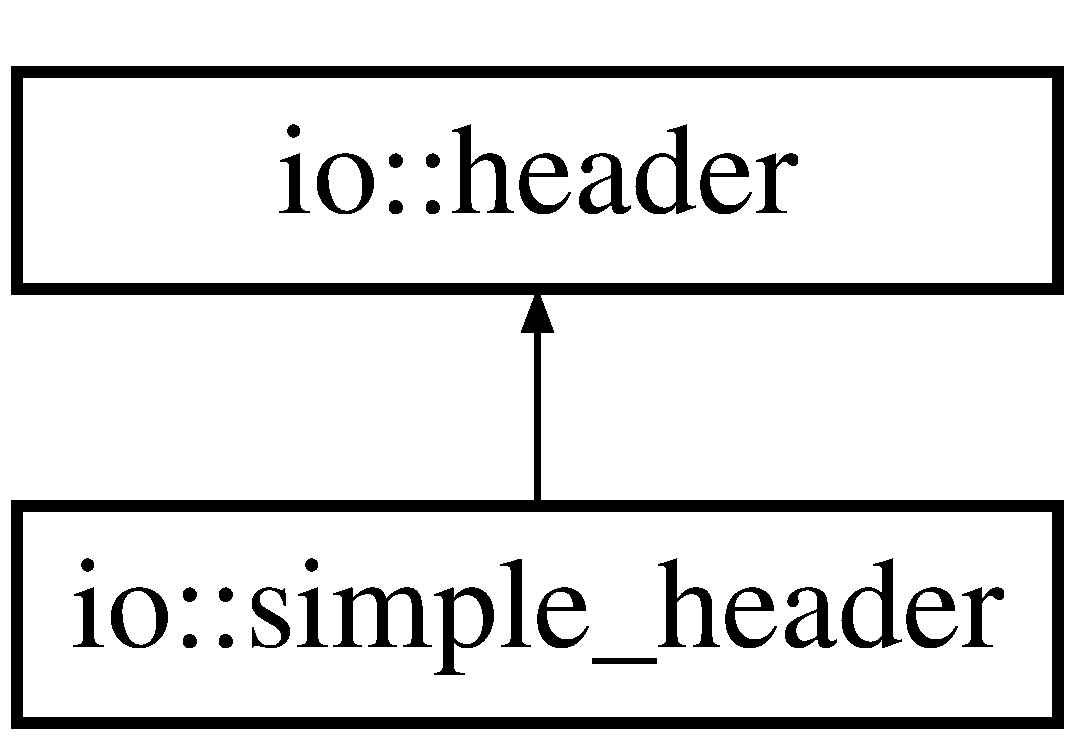
\includegraphics[height=2.000000cm]{classio_1_1simple__header}
\end{center}
\end{figure}
\subsection*{Public Member Functions}
\begin{DoxyCompactItemize}
\item 
\hyperlink{classio_1_1simple__header_acc91be33c4fc1456e670d30a64a1ec72}{simple\-\_\-header} (int i\-\_\-n\-\_\-data\-\_\-headers, std\-::string $\ast$i\-\_\-data\-\_\-headers, std\-::string i\-\_\-comment\-\_\-string=\char`\"{}\#\char`\"{})
\item 
std\-::string \hyperlink{classio_1_1simple__header_a24e9f310d5a022872ef315204e4b0add}{output\-\_\-header} ()
\begin{DoxyCompactList}\small\item\em Make the header for the output file. \end{DoxyCompactList}\end{DoxyCompactItemize}


\subsection{Detailed Description}
A simple header class. 



 This class generates a simple header that contains just the names of the columns. 

\subsection{Constructor \& Destructor Documentation}
\hypertarget{classio_1_1simple__header_acc91be33c4fc1456e670d30a64a1ec72}{\index{io\-::simple\-\_\-header@{io\-::simple\-\_\-header}!simple\-\_\-header@{simple\-\_\-header}}
\index{simple\-\_\-header@{simple\-\_\-header}!io::simple_header@{io\-::simple\-\_\-header}}
\subsubsection[{simple\-\_\-header}]{\setlength{\rightskip}{0pt plus 5cm}io\-::simple\-\_\-header\-::simple\-\_\-header (
\begin{DoxyParamCaption}
\item[{int}]{i\-\_\-n\-\_\-data\-\_\-headers, }
\item[{std\-::string $\ast$}]{i\-\_\-data\-\_\-headers, }
\item[{std\-::string}]{i\-\_\-comment\-\_\-string = {\ttfamily \char`\"{}\#\char`\"{}}}
\end{DoxyParamCaption}
)}}\label{classio_1_1simple__header_acc91be33c4fc1456e670d30a64a1ec72}


 
\begin{DoxyParams}{Parameters}
{\em i\-\_\-n\-\_\-data\-\_\-headers} & An integer number of column headers to be read from i\-\_\-data\-\_\-headers \\
\hline
{\em i\-\_\-data\-\_\-headers} & An array of strings that are the column headers \\
\hline
{\em i\-\_\-comment\-\_\-string} & The string to be used as the comment before the header lines \\
\hline
\end{DoxyParams}


\subsection{Member Function Documentation}
\hypertarget{classio_1_1simple__header_a24e9f310d5a022872ef315204e4b0add}{\index{io\-::simple\-\_\-header@{io\-::simple\-\_\-header}!output\-\_\-header@{output\-\_\-header}}
\index{output\-\_\-header@{output\-\_\-header}!io::simple_header@{io\-::simple\-\_\-header}}
\subsubsection[{output\-\_\-header}]{\setlength{\rightskip}{0pt plus 5cm}std\-::string io\-::simple\-\_\-header\-::output\-\_\-header (
\begin{DoxyParamCaption}
{}
\end{DoxyParamCaption}
)\hspace{0.3cm}{\ttfamily [inline]}, {\ttfamily [virtual]}}}\label{classio_1_1simple__header_a24e9f310d5a022872ef315204e4b0add}


Make the header for the output file. 



 \begin{DoxyReturn}{Returns}
The string to be streamed to the output file 
\end{DoxyReturn}


Reimplemented from \hyperlink{classio_1_1header_af7535d58a31712cdfb753ab0f19626f1}{io\-::header}.



The documentation for this class was generated from the following files\-:\begin{DoxyCompactItemize}
\item 
/\-Users/justinbrown/\-Dropbox/spectral\-\_\-element/src/utils/\hyperlink{io_8hpp}{io.\-hpp}\item 
/\-Users/justinbrown/\-Dropbox/spectral\-\_\-element/src/utils/\hyperlink{io_8cpp}{io.\-cpp}\end{DoxyCompactItemize}

\hypertarget{classio_1_1simple__output}{\section{io\-:\-:simple\-\_\-output Class Reference}
\label{classio_1_1simple__output}\index{io\-::simple\-\_\-output@{io\-::simple\-\_\-output}}
}


A simple implementation of the output class.  




{\ttfamily \#include $<$io.\-hpp$>$}

Inheritance diagram for io\-:\-:simple\-\_\-output\-:\begin{figure}[H]
\begin{center}
\leavevmode
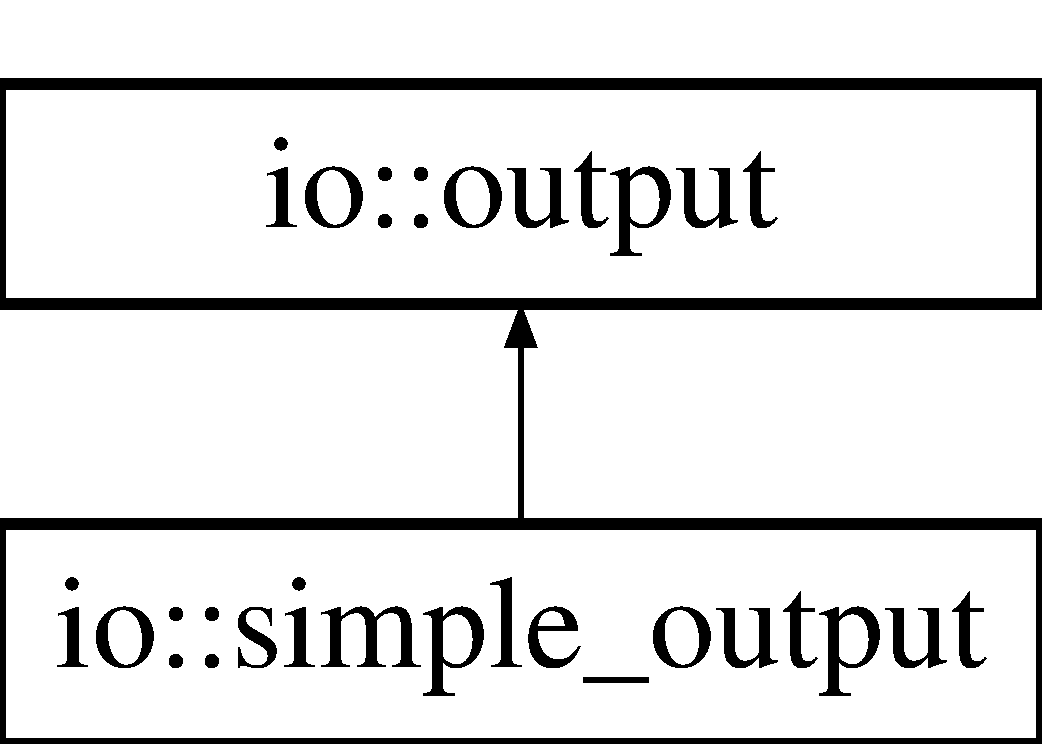
\includegraphics[height=2.000000cm]{classio_1_1simple__output}
\end{center}
\end{figure}
\subsection*{Public Member Functions}
\begin{DoxyCompactItemize}
\item 
\hyperlink{classio_1_1simple__output_a7b4c7960b14193d6bd7756c1c9f0f3b4}{simple\-\_\-output} (std\-::string i\-\_\-file\-\_\-name, int i\-\_\-n, int i\-\_\-output\-\_\-every=1)
\item 
void \hyperlink{classio_1_1simple__output_ab0af023314775f6e9e3bf08ee3cc83f9}{to\-\_\-file} ()
\begin{DoxyCompactList}\small\item\em Outputs to file\-\_\-name. \end{DoxyCompactList}\end{DoxyCompactItemize}
\subsection*{Additional Inherited Members}


\subsection{Detailed Description}
A simple implementation of the output class. 



 This class is a simple implementation of the output class. 

\subsection{Constructor \& Destructor Documentation}
\hypertarget{classio_1_1simple__output_a7b4c7960b14193d6bd7756c1c9f0f3b4}{\index{io\-::simple\-\_\-output@{io\-::simple\-\_\-output}!simple\-\_\-output@{simple\-\_\-output}}
\index{simple\-\_\-output@{simple\-\_\-output}!io::simple_output@{io\-::simple\-\_\-output}}
\subsubsection[{simple\-\_\-output}]{\setlength{\rightskip}{0pt plus 5cm}io\-::simple\-\_\-output\-::simple\-\_\-output (
\begin{DoxyParamCaption}
\item[{std\-::string}]{i\-\_\-file\-\_\-name, }
\item[{int}]{i\-\_\-n, }
\item[{int}]{i\-\_\-output\-\_\-every = {\ttfamily 1}}
\end{DoxyParamCaption}
)\hspace{0.3cm}{\ttfamily [inline]}}}\label{classio_1_1simple__output_a7b4c7960b14193d6bd7756c1c9f0f3b4}


 
\begin{DoxyParams}{Parameters}
{\em i\-\_\-file\-\_\-name} & The string name of file for output \\
\hline
{\em i\-\_\-n} & The integer number of points in the data \\
\hline
{\em i\-\_\-output\-\_\-every} & An integer number of steps between outputs \\
\hline
\end{DoxyParams}


\subsection{Member Function Documentation}
\hypertarget{classio_1_1simple__output_ab0af023314775f6e9e3bf08ee3cc83f9}{\index{io\-::simple\-\_\-output@{io\-::simple\-\_\-output}!to\-\_\-file@{to\-\_\-file}}
\index{to\-\_\-file@{to\-\_\-file}!io::simple_output@{io\-::simple\-\_\-output}}
\subsubsection[{to\-\_\-file}]{\setlength{\rightskip}{0pt plus 5cm}void io\-::simple\-\_\-output\-::to\-\_\-file (
\begin{DoxyParamCaption}
{}
\end{DoxyParamCaption}
)\hspace{0.3cm}{\ttfamily [inline]}, {\ttfamily [virtual]}}}\label{classio_1_1simple__output_ab0af023314775f6e9e3bf08ee3cc83f9}


Outputs to file\-\_\-name. 



 

Implements \hyperlink{classio_1_1output_aae295dd37ca6397fcf8c2109f2c0e418}{io\-::output}.



The documentation for this class was generated from the following file\-:\begin{DoxyCompactItemize}
\item 
/\-Users/justinbrown/\-Dropbox/spectral\-\_\-element/src/utils/\hyperlink{io_8hpp}{io.\-hpp}\end{DoxyCompactItemize}

\hypertarget{classbases_1_1solver}{\section{bases\-:\-:solver Class Reference}
\label{classbases_1_1solver}\index{bases\-::solver@{bases\-::solver}}
}


A class designed to solve a matrix equation.  




{\ttfamily \#include $<$solver.\-hpp$>$}

Inheritance diagram for bases\-:\-:solver\-:\begin{figure}[H]
\begin{center}
\leavevmode
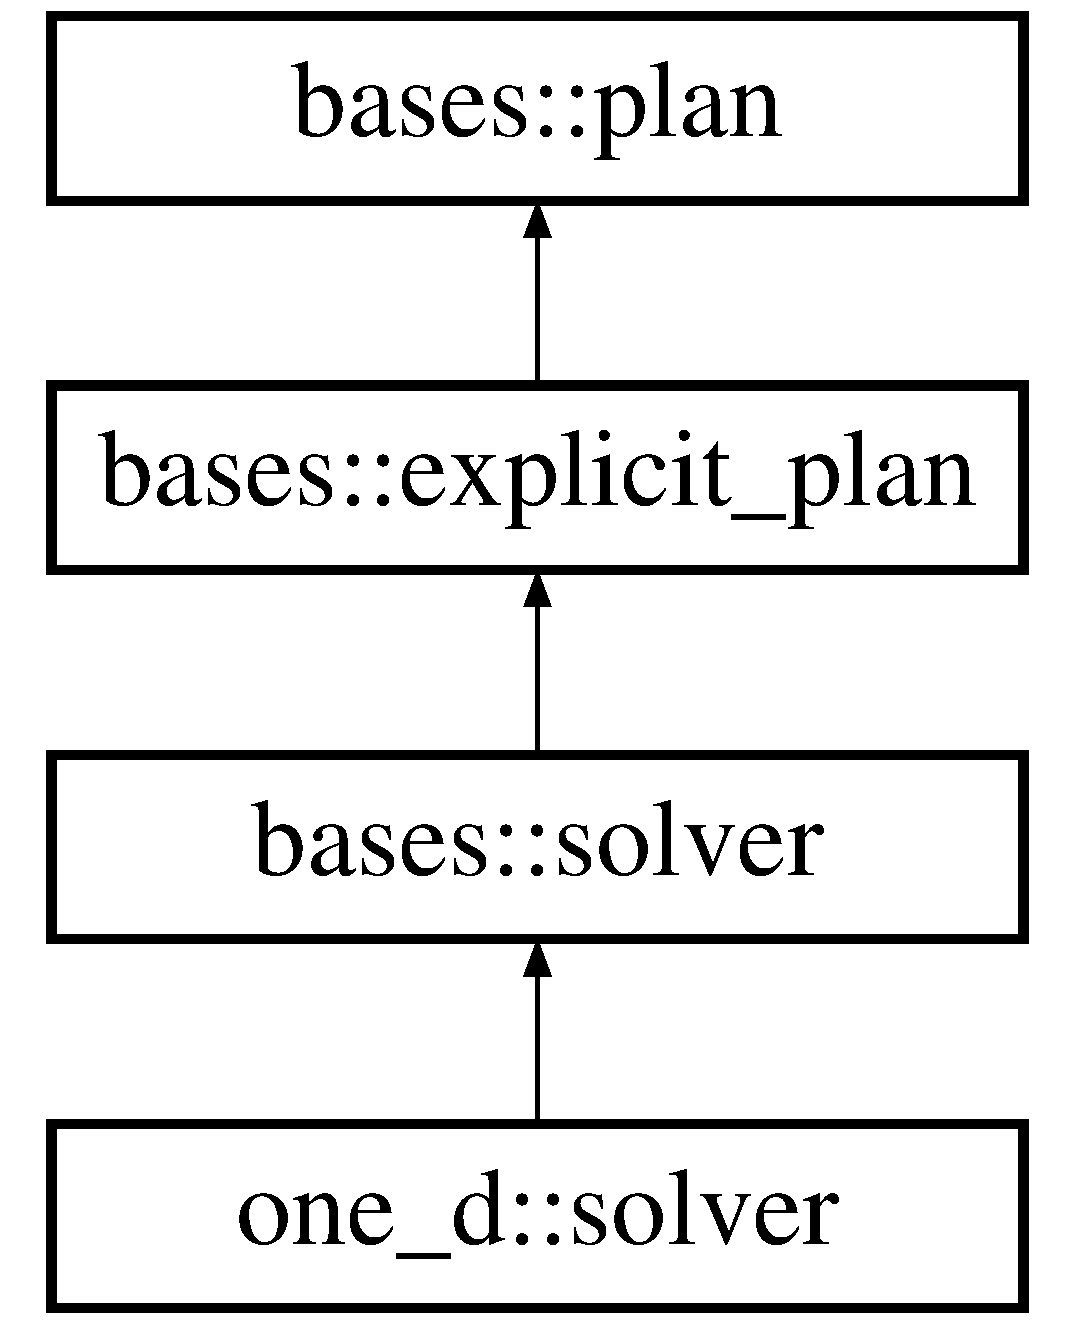
\includegraphics[height=4.000000cm]{classbases_1_1solver}
\end{center}
\end{figure}
\subsection*{Public Member Functions}
\begin{DoxyCompactItemize}
\item 
\hyperlink{classbases_1_1solver_a7b849e5ddfd8ae55b4bbf59010d2b4bd}{solver} (\hyperlink{classbases_1_1element}{element} $\ast$i\-\_\-element\-\_\-ptr, int i\-\_\-n, int i\-\_\-name\-\_\-in, int i\-\_\-name\-\_\-out, int i\-\_\-flags=0x00)
\begin{DoxyCompactList}\small\item\em \end{DoxyCompactList}\item 
virtual void \hyperlink{classbases_1_1solver_a8adf4c428bf4322a664c811073b491e1}{execute} ()
\begin{DoxyCompactList}\small\item\em Solve the matrix equation. \end{DoxyCompactList}\end{DoxyCompactItemize}
\subsection*{Protected Member Functions}
\begin{DoxyCompactItemize}
\item 
virtual void \hyperlink{classbases_1_1solver_adfc4b2709650924535e117405e7e3a21}{factorize} ()
\begin{DoxyCompactList}\small\item\em Factorize the matrix equation. \end{DoxyCompactList}\end{DoxyCompactItemize}
\subsection*{Additional Inherited Members}


\subsection{Detailed Description}
A class designed to solve a matrix equation. 



 

\subsection{Constructor \& Destructor Documentation}
\hypertarget{classbases_1_1solver_a7b849e5ddfd8ae55b4bbf59010d2b4bd}{\index{bases\-::solver@{bases\-::solver}!solver@{solver}}
\index{solver@{solver}!bases::solver@{bases\-::solver}}
\subsubsection[{solver}]{\setlength{\rightskip}{0pt plus 5cm}bases\-::solver\-::solver (
\begin{DoxyParamCaption}
\item[{{\bf element} $\ast$}]{i\-\_\-element\-\_\-ptr, }
\item[{int}]{i\-\_\-n, }
\item[{int}]{i\-\_\-name\-\_\-in, }
\item[{int}]{i\-\_\-name\-\_\-out, }
\item[{int}]{i\-\_\-flags = {\ttfamily 0x00}}
\end{DoxyParamCaption}
)\hspace{0.3cm}{\ttfamily [inline]}}}\label{classbases_1_1solver_a7b849e5ddfd8ae55b4bbf59010d2b4bd}






 

 
\begin{DoxyParams}{Parameters}
{\em i\-\_\-n} & The integer number of elements in the data \\
\hline
{\em i\-\_\-name\-\_\-in} & The integer scalar index of the input \\
\hline
{\em i\-\_\-name\-\_\-out} & The integer scalar index of the output \\
\hline
\end{DoxyParams}


 
\begin{DoxyParams}{Parameters}
{\em i\-\_\-element\-\_\-ptr} & A pointer to the associated element \\
\hline
\end{DoxyParams}


\subsection{Member Function Documentation}
\hypertarget{classbases_1_1solver_a8adf4c428bf4322a664c811073b491e1}{\index{bases\-::solver@{bases\-::solver}!execute@{execute}}
\index{execute@{execute}!bases::solver@{bases\-::solver}}
\subsubsection[{execute}]{\setlength{\rightskip}{0pt plus 5cm}virtual void bases\-::solver\-::execute (
\begin{DoxyParamCaption}
{}
\end{DoxyParamCaption}
)\hspace{0.3cm}{\ttfamily [inline]}, {\ttfamily [virtual]}}}\label{classbases_1_1solver_a8adf4c428bf4322a664c811073b491e1}


Solve the matrix equation. 



 

Reimplemented from \hyperlink{classbases_1_1explicit__plan_a21bcba4d429590031bba41ee2a48a4ef}{bases\-::explicit\-\_\-plan}.



Reimplemented in \hyperlink{classone__d_1_1solver_a7c28bd733cb3c3849afe1773974eb4f6}{one\-\_\-d\-::solver}.

\hypertarget{classbases_1_1solver_adfc4b2709650924535e117405e7e3a21}{\index{bases\-::solver@{bases\-::solver}!factorize@{factorize}}
\index{factorize@{factorize}!bases::solver@{bases\-::solver}}
\subsubsection[{factorize}]{\setlength{\rightskip}{0pt plus 5cm}virtual void bases\-::solver\-::factorize (
\begin{DoxyParamCaption}
{}
\end{DoxyParamCaption}
)\hspace{0.3cm}{\ttfamily [inline]}, {\ttfamily [protected]}, {\ttfamily [virtual]}}}\label{classbases_1_1solver_adfc4b2709650924535e117405e7e3a21}


Factorize the matrix equation. 



 This method checks first whether the matrix has been factorized, according to the execution flags. Upon success, it notes in the execution flags that the matrix has been factorized. 

Reimplemented in \hyperlink{classone__d_1_1solver_a33e9bc05b91b4da54ce783235447f334}{one\-\_\-d\-::solver}.



The documentation for this class was generated from the following file\-:\begin{DoxyCompactItemize}
\item 
/\-Users/justinbrown/\-Dropbox/spectral\-\_\-element/src/bases/\hyperlink{solver_8hpp}{solver.\-hpp}\end{DoxyCompactItemize}

\hypertarget{classone__d_1_1solver}{\section{one\-\_\-d\-:\-:solver Class Reference}
\label{classone__d_1_1solver}\index{one\-\_\-d\-::solver@{one\-\_\-d\-::solver}}
}


A 1\-D implementation of a matrix solver.  




{\ttfamily \#include $<$solver\-\_\-one\-\_\-d.\-hpp$>$}

Inheritance diagram for one\-\_\-d\-:\-:solver\-:\begin{figure}[H]
\begin{center}
\leavevmode
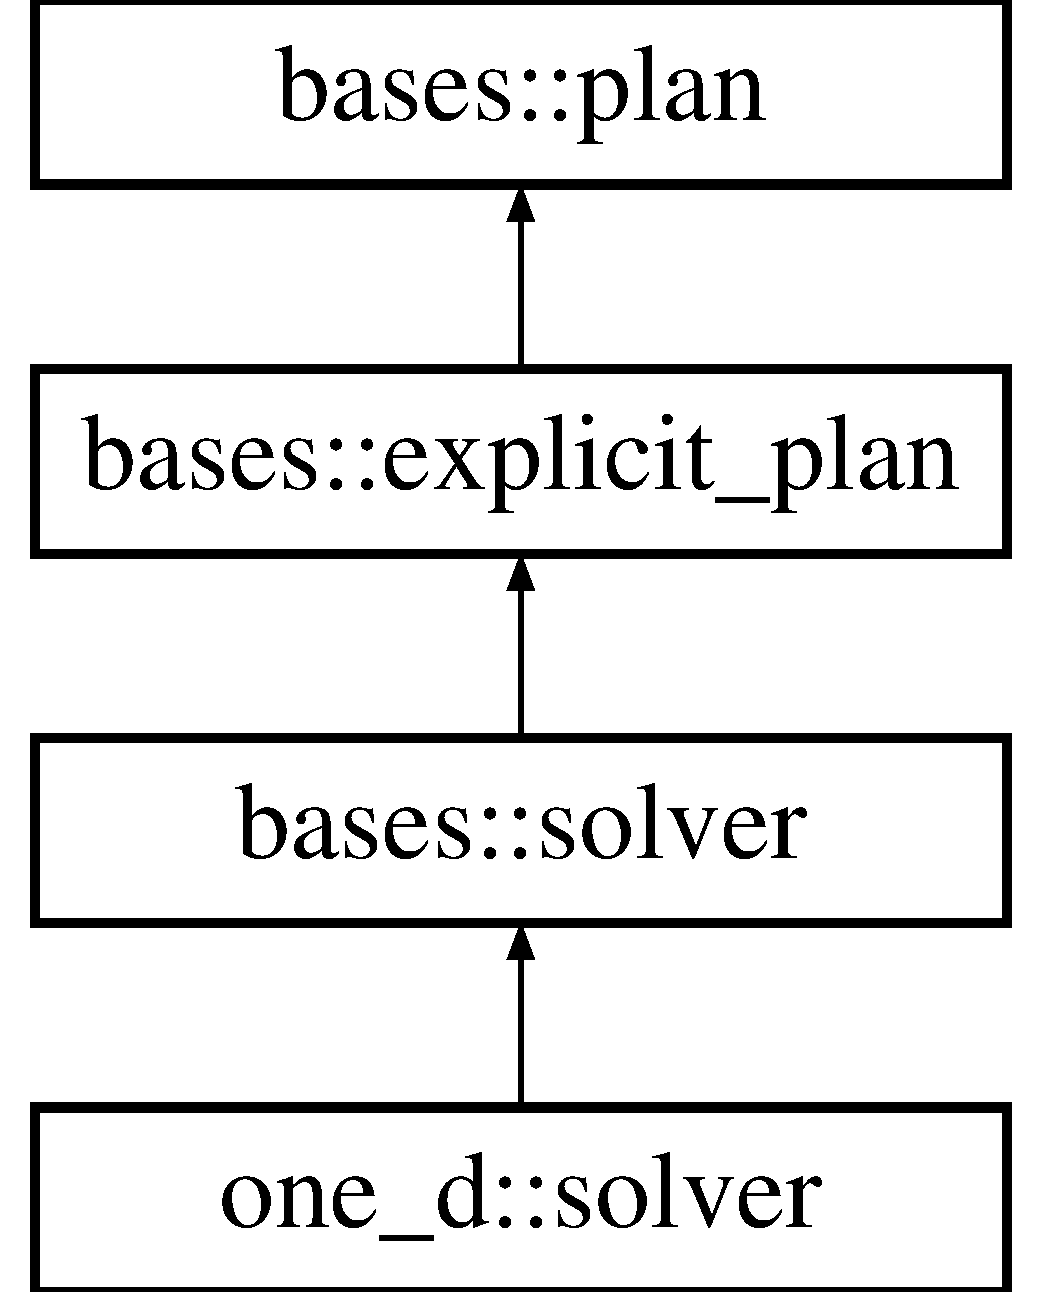
\includegraphics[height=4.000000cm]{classone__d_1_1solver}
\end{center}
\end{figure}
\subsection*{Public Member Functions}
\begin{DoxyCompactItemize}
\item 
\hyperlink{classone__d_1_1solver_a17c2b3e1be15e2311ac36de12cfb877b}{solver} (\hyperlink{classbases_1_1element}{bases\-::element} $\ast$i\-\_\-element\-\_\-ptr, int i\-\_\-n, int i\-\_\-excess\-\_\-0, int i\-\_\-excess\-\_\-n, double \&i\-\_\-timestep, double \&i\-\_\-alpha\-\_\-0, double \&i\-\_\-alpha\-\_\-n, double $\ast$i\-\_\-default\-\_\-matrix, double $\ast$i\-\_\-matrix, int i\-\_\-name\-\_\-in, int i\-\_\-name\-\_\-rhs, int i\-\_\-name\-\_\-out=null, int i\-\_\-flags=0x00)
\begin{DoxyCompactList}\small\item\em \end{DoxyCompactList}\item 
void \hyperlink{classone__d_1_1solver_a7c28bd733cb3c3849afe1773974eb4f6}{execute} ()
\begin{DoxyCompactList}\small\item\em Solve the matrix equation. \end{DoxyCompactList}\end{DoxyCompactItemize}
\subsection*{Protected Member Functions}
\begin{DoxyCompactItemize}
\item 
void \hyperlink{classone__d_1_1solver_a33e9bc05b91b4da54ce783235447f334}{factorize} ()
\begin{DoxyCompactList}\small\item\em Factorize the matrix equation. \end{DoxyCompactList}\end{DoxyCompactItemize}
\subsection*{Protected Attributes}
\begin{DoxyCompactItemize}
\item 
\hypertarget{classone__d_1_1solver_a490325a537d8addf5edea22b7ae4c4f5}{double \& \hyperlink{classone__d_1_1solver_a490325a537d8addf5edea22b7ae4c4f5}{timestep}}\label{classone__d_1_1solver_a490325a537d8addf5edea22b7ae4c4f5}

\begin{DoxyCompactList}\small\item\em A double reference to the current timestep. \end{DoxyCompactList}\item 
\hypertarget{classone__d_1_1solver_aa38c2e7d7f91ab64f3de449ad4f0c5c8}{double \& \hyperlink{classone__d_1_1solver_aa38c2e7d7f91ab64f3de449ad4f0c5c8}{alpha\-\_\-0}}\label{classone__d_1_1solver_aa38c2e7d7f91ab64f3de449ad4f0c5c8}

\begin{DoxyCompactList}\small\item\em A double reference to the current edge\-\_\-0 weight. \end{DoxyCompactList}\item 
\hypertarget{classone__d_1_1solver_a3e383f0bfc5e541f22583110eae4c9ab}{double \& \hyperlink{classone__d_1_1solver_a3e383f0bfc5e541f22583110eae4c9ab}{alpha\-\_\-n}}\label{classone__d_1_1solver_a3e383f0bfc5e541f22583110eae4c9ab}

\begin{DoxyCompactList}\small\item\em A double reference to the current edge\-\_\-n weight. \end{DoxyCompactList}\item 
\hypertarget{classone__d_1_1solver_a07b2fb5dd4cffd6acc7c4e641173c444}{int \hyperlink{classone__d_1_1solver_a07b2fb5dd4cffd6acc7c4e641173c444}{excess\-\_\-0}}\label{classone__d_1_1solver_a07b2fb5dd4cffd6acc7c4e641173c444}

\begin{DoxyCompactList}\small\item\em The integer number of elements to recv from edge\-\_\-0. \end{DoxyCompactList}\item 
\hypertarget{classone__d_1_1solver_a3d3f3a518faff396383fcbad9bed4da2}{int \hyperlink{classone__d_1_1solver_a3d3f3a518faff396383fcbad9bed4da2}{excess\-\_\-n}}\label{classone__d_1_1solver_a3d3f3a518faff396383fcbad9bed4da2}

\begin{DoxyCompactList}\small\item\em The integer number of elements to recv from edge\-\_\-n. \end{DoxyCompactList}\item 
\hypertarget{classone__d_1_1solver_ad9d68340476561f45d2c16226e65099d}{int \hyperlink{classone__d_1_1solver_ad9d68340476561f45d2c16226e65099d}{expected\-\_\-excess\-\_\-0}}\label{classone__d_1_1solver_ad9d68340476561f45d2c16226e65099d}

\begin{DoxyCompactList}\small\item\em The integer number of elements to send to edge\-\_\-0. \end{DoxyCompactList}\item 
\hypertarget{classone__d_1_1solver_a70da7ebd7e0c567586de45fbf28bfb8a}{int \hyperlink{classone__d_1_1solver_a70da7ebd7e0c567586de45fbf28bfb8a}{expected\-\_\-excess\-\_\-n}}\label{classone__d_1_1solver_a70da7ebd7e0c567586de45fbf28bfb8a}

\begin{DoxyCompactList}\small\item\em The integer number of elements to send to edge\-\_\-n. \end{DoxyCompactList}\item 
\hypertarget{classone__d_1_1solver_a9a37e318c74debf5210a52f781b1c1e7}{double $\ast$ \hyperlink{classone__d_1_1solver_a9a37e318c74debf5210a52f781b1c1e7}{rhs}}\label{classone__d_1_1solver_a9a37e318c74debf5210a52f781b1c1e7}

\begin{DoxyCompactList}\small\item\em The double array of the right-\/hand-\/side of the matrix equation. \end{DoxyCompactList}\item 
\hypertarget{classone__d_1_1solver_ac1002a2062ffc61df2ceddbd7d8d3f6e}{double $\ast$ \hyperlink{classone__d_1_1solver_ac1002a2062ffc61df2ceddbd7d8d3f6e}{default\-\_\-matrix}}\label{classone__d_1_1solver_ac1002a2062ffc61df2ceddbd7d8d3f6e}

\begin{DoxyCompactList}\small\item\em The double array of the non-\/timestep dependent matrix component. \end{DoxyCompactList}\item 
\hypertarget{classone__d_1_1solver_a7479d423e0d42293c9d953783f7715df}{double $\ast$ \hyperlink{classone__d_1_1solver_a7479d423e0d42293c9d953783f7715df}{matrix}}\label{classone__d_1_1solver_a7479d423e0d42293c9d953783f7715df}

\begin{DoxyCompactList}\small\item\em The double array of the matrix component to be timestep-\/multiplied. \end{DoxyCompactList}\item 
\hypertarget{classone__d_1_1solver_ab6cae4cf1e23a2e50b40d03ca146833b}{std\-::vector$<$ double $>$ \hyperlink{classone__d_1_1solver_ab6cae4cf1e23a2e50b40d03ca146833b}{error\-\_\-0}}\label{classone__d_1_1solver_ab6cae4cf1e23a2e50b40d03ca146833b}

\begin{DoxyCompactList}\small\item\em A double vector to be recved from edge\-\_\-0. \end{DoxyCompactList}\item 
\hypertarget{classone__d_1_1solver_ae8898a6ede0f1daad9754364a267b7ae}{std\-::vector$<$ double $>$ \hyperlink{classone__d_1_1solver_ae8898a6ede0f1daad9754364a267b7ae}{error\-\_\-n}}\label{classone__d_1_1solver_ae8898a6ede0f1daad9754364a267b7ae}

\begin{DoxyCompactList}\small\item\em A double vector to be recved from edge\-\_\-n. \end{DoxyCompactList}\item 
\hypertarget{classone__d_1_1solver_abb22af2fc401d3ed93ae3f400028c9de}{std\-::vector$<$ double $>$ \hyperlink{classone__d_1_1solver_abb22af2fc401d3ed93ae3f400028c9de}{out\-\_\-error\-\_\-0}}\label{classone__d_1_1solver_abb22af2fc401d3ed93ae3f400028c9de}

\begin{DoxyCompactList}\small\item\em A double vector to be sent to edge\-\_\-0. \end{DoxyCompactList}\item 
\hypertarget{classone__d_1_1solver_ab1ed5c7ce3f6ec0bdc9a6eb8cefaf507}{std\-::vector$<$ double $>$ \hyperlink{classone__d_1_1solver_ab1ed5c7ce3f6ec0bdc9a6eb8cefaf507}{out\-\_\-error\-\_\-n}}\label{classone__d_1_1solver_ab1ed5c7ce3f6ec0bdc9a6eb8cefaf507}

\begin{DoxyCompactList}\small\item\em A double vector to be sent to edge\-\_\-n. \end{DoxyCompactList}\item 
\hypertarget{classone__d_1_1solver_aac1795dc7503b6c96b5c6ad59fc9de20}{std\-::vector$<$ double $>$ \hyperlink{classone__d_1_1solver_aac1795dc7503b6c96b5c6ad59fc9de20}{data\-\_\-temp}}\label{classone__d_1_1solver_aac1795dc7503b6c96b5c6ad59fc9de20}

\begin{DoxyCompactList}\small\item\em A double vector to be used in lieu of data\-\_\-out for non-\/updating steps. \end{DoxyCompactList}\item 
\hypertarget{classone__d_1_1solver_ad34bc1962465a7030a22c825d9fa7473}{std\-::vector$<$ double $>$ \hyperlink{classone__d_1_1solver_ad34bc1962465a7030a22c825d9fa7473}{positions\-\_\-0}}\label{classone__d_1_1solver_ad34bc1962465a7030a22c825d9fa7473}

\begin{DoxyCompactList}\small\item\em A double vector of excess positions from edge\-\_\-0. \end{DoxyCompactList}\item 
\hypertarget{classone__d_1_1solver_a63b789bf32c435c56d4874589fdc81f3}{std\-::vector$<$ double $>$ \hyperlink{classone__d_1_1solver_a63b789bf32c435c56d4874589fdc81f3}{positions\-\_\-n}}\label{classone__d_1_1solver_a63b789bf32c435c56d4874589fdc81f3}

\begin{DoxyCompactList}\small\item\em A double vector of excess positions from edge\-\_\-n. \end{DoxyCompactList}\item 
\hypertarget{classone__d_1_1solver_a422a65f49ae474f7f3a30d1eaca19641}{std\-::vector$<$ double $>$ \hyperlink{classone__d_1_1solver_a422a65f49ae474f7f3a30d1eaca19641}{factorized\-\_\-matrix}}\label{classone__d_1_1solver_a422a65f49ae474f7f3a30d1eaca19641}

\begin{DoxyCompactList}\small\item\em A double vector containing the factorized sum of default matrix and timestep $\ast$ matrix. \end{DoxyCompactList}\item 
\hypertarget{classone__d_1_1solver_a668a33255403a66f8f44167fbf55f009}{std\-::vector$<$ int $>$ \hyperlink{classone__d_1_1solver_a668a33255403a66f8f44167fbf55f009}{ipiv}}\label{classone__d_1_1solver_a668a33255403a66f8f44167fbf55f009}

\begin{DoxyCompactList}\small\item\em A vector of integers needed to calculate the factorization. \end{DoxyCompactList}\end{DoxyCompactItemize}


\subsection{Detailed Description}
A 1\-D implementation of a matrix solver. 



 This matrix solver solves a matrix in each element individually and sends the results to the adjacent elements. This solver should be iterated. 

\subsection{Constructor \& Destructor Documentation}
\hypertarget{classone__d_1_1solver_a17c2b3e1be15e2311ac36de12cfb877b}{\index{one\-\_\-d\-::solver@{one\-\_\-d\-::solver}!solver@{solver}}
\index{solver@{solver}!one_d::solver@{one\-\_\-d\-::solver}}
\subsubsection[{solver}]{\setlength{\rightskip}{0pt plus 5cm}one\-\_\-d\-::solver\-::solver (
\begin{DoxyParamCaption}
\item[{{\bf bases\-::element} $\ast$}]{i\-\_\-element\-\_\-ptr, }
\item[{int}]{i\-\_\-n, }
\item[{int}]{i\-\_\-excess\-\_\-0, }
\item[{int}]{i\-\_\-excess\-\_\-n, }
\item[{double \&}]{i\-\_\-timestep, }
\item[{double \&}]{i\-\_\-alpha\-\_\-0, }
\item[{double \&}]{i\-\_\-alpha\-\_\-n, }
\item[{double $\ast$}]{i\-\_\-default\-\_\-matrix, }
\item[{double $\ast$}]{i\-\_\-matrix, }
\item[{int}]{i\-\_\-name\-\_\-in, }
\item[{int}]{i\-\_\-name\-\_\-rhs, }
\item[{int}]{i\-\_\-name\-\_\-out = {\ttfamily null}, }
\item[{int}]{i\-\_\-flags = {\ttfamily 0x00}}
\end{DoxyParamCaption}
)}}\label{classone__d_1_1solver_a17c2b3e1be15e2311ac36de12cfb877b}






 
\begin{DoxyParams}{Parameters}
{\em i\-\_\-excess\-\_\-0} & The integer number of excess elements on the edge\-\_\-0 side \\
\hline
{\em i\-\_\-excess\-\_\-n} & The integer number of excess elements on the edge\-\_\-n side \\
\hline
{\em i\-\_\-timestep} & A double reference to the current timestep \\
\hline
{\em i\-\_\-alpha\-\_\-0} & A double reference to the edge\-\_\-0 weight \\
\hline
{\em i\-\_\-alpha\-\_\-n} & A double reference to the edge\-\_\-n weight \\
\hline
{\em i\-\_\-default\-\_\-matrix} & A double array containing the 0 order collocation matrix \\
\hline
{\em i\-\_\-matrix} & The double matrix to be factorized \\
\hline
{\em i\-\_\-name\-\_\-rhs} & The integer representation of the matrix right-\/hand-\/side \\
\hline
\end{DoxyParams}


 

 
\begin{DoxyParams}{Parameters}
{\em i\-\_\-n} & The integer number of elements in the data \\
\hline
{\em i\-\_\-name\-\_\-in} & The integer scalar index of the input \\
\hline
{\em i\-\_\-name\-\_\-out} & The integer scalar index of the output \\
\hline
\end{DoxyParams}


 
\begin{DoxyParams}{Parameters}
{\em i\-\_\-element\-\_\-ptr} & A pointer to the associated element \\
\hline
\end{DoxyParams}


\subsection{Member Function Documentation}
\hypertarget{classone__d_1_1solver_a7c28bd733cb3c3849afe1773974eb4f6}{\index{one\-\_\-d\-::solver@{one\-\_\-d\-::solver}!execute@{execute}}
\index{execute@{execute}!one_d::solver@{one\-\_\-d\-::solver}}
\subsubsection[{execute}]{\setlength{\rightskip}{0pt plus 5cm}void one\-\_\-d\-::solver\-::execute (
\begin{DoxyParamCaption}
{}
\end{DoxyParamCaption}
)\hspace{0.3cm}{\ttfamily [virtual]}}}\label{classone__d_1_1solver_a7c28bd733cb3c3849afe1773974eb4f6}


Solve the matrix equation. 



 

 

Reimplemented from \hyperlink{classbases_1_1solver_a8adf4c428bf4322a664c811073b491e1}{bases\-::solver}.

\hypertarget{classone__d_1_1solver_a33e9bc05b91b4da54ce783235447f334}{\index{one\-\_\-d\-::solver@{one\-\_\-d\-::solver}!factorize@{factorize}}
\index{factorize@{factorize}!one_d::solver@{one\-\_\-d\-::solver}}
\subsubsection[{factorize}]{\setlength{\rightskip}{0pt plus 5cm}void one\-\_\-d\-::solver\-::factorize (
\begin{DoxyParamCaption}
{}
\end{DoxyParamCaption}
)\hspace{0.3cm}{\ttfamily [protected]}, {\ttfamily [virtual]}}}\label{classone__d_1_1solver_a33e9bc05b91b4da54ce783235447f334}


Factorize the matrix equation. 



 

 This method checks first whether the matrix has been factorized, according to the execution flags. Upon success, it notes in the execution flags that the matrix has been factorized. 

Reimplemented from \hyperlink{classbases_1_1solver_adfc4b2709650924535e117405e7e3a21}{bases\-::solver}.



The documentation for this class was generated from the following files\-:\begin{DoxyCompactItemize}
\item 
/\-Users/justinbrown/\-Dropbox/spectral\-\_\-element/src/one\-\_\-d/solver\-\_\-one\-\_\-d.\-hpp\item 
/\-Users/justinbrown/\-Dropbox/spectral\-\_\-element/src/one\-\_\-d/\hyperlink{solver__one__d_8cpp}{solver\-\_\-one\-\_\-d.\-cpp}\end{DoxyCompactItemize}

\hypertarget{unionio_1_1types}{\section{io\-:\-:types Union Reference}
\label{unionio_1_1types}\index{io\-::types@{io\-::types}}
}


A class for reading experiment parameters out of a parameter file.  




{\ttfamily \#include $<$io.\-hpp$>$}

\subsection*{Public Member Functions}
\begin{DoxyCompactItemize}
\item 
\hypertarget{unionio_1_1types_a91a6efe8a35b62181d858c919efc7948}{{\bfseries types} (int in)}\label{unionio_1_1types_a91a6efe8a35b62181d858c919efc7948}

\item 
\hypertarget{unionio_1_1types_a9d790549cd44ef300795179e51e2a54c}{{\bfseries types} (double in)}\label{unionio_1_1types_a9d790549cd44ef300795179e51e2a54c}

\item 
\hypertarget{unionio_1_1types_abbfc93592643c93666dcd37e50e110cd}{{\bfseries operator int} ()}\label{unionio_1_1types_abbfc93592643c93666dcd37e50e110cd}

\item 
\hypertarget{unionio_1_1types_aaddbc2205d65298d88da12a752143993}{{\bfseries operator double} ()}\label{unionio_1_1types_aaddbc2205d65298d88da12a752143993}

\end{DoxyCompactItemize}
\subsection*{Public Attributes}
\begin{DoxyCompactItemize}
\item 
\hypertarget{unionio_1_1types_aeb447411e6614731ea94a680fa06a16e}{unsigned long {\bfseries as\-U\-Long}}\label{unionio_1_1types_aeb447411e6614731ea94a680fa06a16e}

\item 
\hypertarget{unionio_1_1types_ac496701aa202e7561482839eff444ed6}{int {\bfseries as\-Int}}\label{unionio_1_1types_ac496701aa202e7561482839eff444ed6}

\item 
\hypertarget{unionio_1_1types_a02cfe6ea6a76b654839f2109e7c5517f}{double {\bfseries as\-Double}}\label{unionio_1_1types_a02cfe6ea6a76b654839f2109e7c5517f}

\end{DoxyCompactItemize}


\subsection{Detailed Description}
A class for reading experiment parameters out of a parameter file. 



 

The documentation for this union was generated from the following file\-:\begin{DoxyCompactItemize}
\item 
/\-Users/justinbrown/\-Dropbox/spectral\-\_\-element/src/utils/\hyperlink{io_8hpp}{io.\-hpp}\end{DoxyCompactItemize}

\chapter{File Documentation}
\hypertarget{collocation_8cpp}{\section{/\-Users/justinbrown/\-Dropbox/spectral\-\_\-element/src/bases/collocation.cpp File Reference}
\label{collocation_8cpp}\index{/\-Users/justinbrown/\-Dropbox/spectral\-\_\-element/src/bases/collocation.\-cpp@{/\-Users/justinbrown/\-Dropbox/spectral\-\_\-element/src/bases/collocation.\-cpp}}
}
{\ttfamily \#include \char`\"{}../config.\-hpp\char`\"{}}\\*
{\ttfamily \#include \char`\"{}collocation.\-hpp\char`\"{}}\\*
\subsection*{Namespaces}
\begin{DoxyCompactItemize}
\item 
namespace \hyperlink{namespacebases}{bases}
\begin{DoxyCompactList}\small\item\em A namespace containing the base classes of the code. \end{DoxyCompactList}\end{DoxyCompactItemize}


\subsection{Detailed Description}




Spectral Element

Created by Justin Brown on 2013-\/04-\/19. Copyright 2013 Justin Brown. All rights reserved. 
\hypertarget{collocation_8hpp}{\section{/\-Users/justinbrown/\-Dropbox/spectral\-\_\-element/src/bases/collocation.hpp File Reference}
\label{collocation_8hpp}\index{/\-Users/justinbrown/\-Dropbox/spectral\-\_\-element/src/bases/collocation.\-hpp@{/\-Users/justinbrown/\-Dropbox/spectral\-\_\-element/src/bases/collocation.\-hpp}}
}
{\ttfamily \#include $<$vector$>$}\\*
{\ttfamily \#include \char`\"{}../config.\-hpp\char`\"{}}\\*
\subsection*{Classes}
\begin{DoxyCompactItemize}
\item 
class \hyperlink{classbases_1_1collocation__grid}{bases\-::collocation\-\_\-grid}
\begin{DoxyCompactList}\small\item\em A class containing a collocation grid. \end{DoxyCompactList}\end{DoxyCompactItemize}
\subsection*{Namespaces}
\begin{DoxyCompactItemize}
\item 
namespace \hyperlink{namespacebases}{bases}
\begin{DoxyCompactList}\small\item\em A namespace containing the base classes of the code. \end{DoxyCompactList}\end{DoxyCompactItemize}


\subsection{Detailed Description}




Spectral Element

Created by Justin Brown on 2013-\/04-\/19. Copyright 2013 Justin Brown. All rights reserved. 
\hypertarget{element_8cpp}{\section{/\-Users/justinbrown/\-Dropbox/spectral\-\_\-element/src/bases/element.cpp File Reference}
\label{element_8cpp}\index{/\-Users/justinbrown/\-Dropbox/spectral\-\_\-element/src/bases/element.\-cpp@{/\-Users/justinbrown/\-Dropbox/spectral\-\_\-element/src/bases/element.\-cpp}}
}
{\ttfamily \#include $<$cassert$>$}\\*
{\ttfamily \#include \char`\"{}element.\-hpp\char`\"{}}\\*
{\ttfamily \#include \char`\"{}../config.\-hpp\char`\"{}}\\*
{\ttfamily \#include \char`\"{}solver.\-hpp\char`\"{}}\\*
{\ttfamily \#include \char`\"{}../utils/utils.\-hpp\char`\"{}}\\*
\subsection*{Namespaces}
\begin{DoxyCompactItemize}
\item 
namespace \hyperlink{namespacebases}{bases}
\begin{DoxyCompactList}\small\item\em A namespace containing the base classes of the code. \end{DoxyCompactList}\end{DoxyCompactItemize}


\subsection{Detailed Description}




Spectral Element

Created by Justin Brown on 2013-\/04-\/19. Copyright 2013 Justin Brown. All rights reserved. 
\hypertarget{element_8hpp}{\section{/\-Users/justinbrown/\-Dropbox/spectral\-\_\-element/src/bases/element.hpp File Reference}
\label{element_8hpp}\index{/\-Users/justinbrown/\-Dropbox/spectral\-\_\-element/src/bases/element.\-hpp@{/\-Users/justinbrown/\-Dropbox/spectral\-\_\-element/src/bases/element.\-hpp}}
}
{\ttfamily \#include $<$string$>$}\\*
{\ttfamily \#include $<$cassert$>$}\\*
{\ttfamily \#include $<$memory$>$}\\*
{\ttfamily \#include \char`\"{}plan.\-hpp\char`\"{}}\\*
{\ttfamily \#include \char`\"{}solver.\-hpp\char`\"{}}\\*
{\ttfamily \#include \char`\"{}../utils/io.\-hpp\char`\"{}}\\*
{\ttfamily \#include \char`\"{}messenger.\-hpp\char`\"{}}\\*
{\ttfamily \#include \char`\"{}collocation.\-hpp\char`\"{}}\\*
{\ttfamily \#include \char`\"{}../config.\-hpp\char`\"{}}\\*
\subsection*{Classes}
\begin{DoxyCompactItemize}
\item 
class \hyperlink{classbases_1_1element}{bases\-::element}
\begin{DoxyCompactList}\small\item\em This is the basic class of the code. \end{DoxyCompactList}\end{DoxyCompactItemize}
\subsection*{Namespaces}
\begin{DoxyCompactItemize}
\item 
namespace \hyperlink{namespacebases}{bases}
\begin{DoxyCompactList}\small\item\em A namespace containing the base classes of the code. \end{DoxyCompactList}\end{DoxyCompactItemize}


\subsection{Detailed Description}




Spectral Element

This file contains the element class, the basic functional unit of the code.

Created by Justin Brown on 2013-\/04-\/19. Copyright 2013 Justin Brown. All rights reserved. 
\hypertarget{messenger_8cpp}{\section{/\-Users/justinbrown/\-Dropbox/spectral\-\_\-element/src/bases/messenger.cpp File Reference}
\label{messenger_8cpp}\index{/\-Users/justinbrown/\-Dropbox/spectral\-\_\-element/src/bases/messenger.\-cpp@{/\-Users/justinbrown/\-Dropbox/spectral\-\_\-element/src/bases/messenger.\-cpp}}
}
{\ttfamily \#include \char`\"{}messenger.\-hpp\char`\"{}}\\*
{\ttfamily \#include $<$cassert$>$}\\*
{\ttfamily \#include $<$algorithm$>$}\\*
{\ttfamily \#include $<$vector$>$}\\*
{\ttfamily \#include \char`\"{}../config.\-hpp\char`\"{}}\\*
{\ttfamily \#include \char`\"{}../utils/utils.\-hpp\char`\"{}}\\*
\subsection*{Namespaces}
\begin{DoxyCompactItemize}
\item 
namespace \hyperlink{namespacebases}{bases}
\begin{DoxyCompactList}\small\item\em A namespace containing the base classes of the code. \end{DoxyCompactList}\end{DoxyCompactItemize}


\subsection{Detailed Description}




/\-Users/justinbrown/\-Dropbox/spectral\-\_\-element

Created by Justin Brown on 2013-\/08-\/17. Copyright 2013 Justin Brown. All rights reserved. 
\hypertarget{messenger_8hpp}{\section{/\-Users/justinbrown/\-Dropbox/spectral\-\_\-element/src/bases/messenger.hpp File Reference}
\label{messenger_8hpp}\index{/\-Users/justinbrown/\-Dropbox/spectral\-\_\-element/src/bases/messenger.\-hpp@{/\-Users/justinbrown/\-Dropbox/spectral\-\_\-element/src/bases/messenger.\-hpp}}
}
{\ttfamily \#include $<$cassert$>$}\\*
{\ttfamily \#include $<$algorithm$>$}\\*
{\ttfamily \#include $<$vector$>$}\\*
{\ttfamily \#include \char`\"{}../config.\-hpp\char`\"{}}\\*
{\ttfamily \#include \char`\"{}../utils/utils.\-hpp\char`\"{}}\\*
\subsection*{Classes}
\begin{DoxyCompactItemize}
\item 
class \hyperlink{classbases_1_1messenger}{bases\-::messenger}
\begin{DoxyCompactList}\small\item\em A class to manage boundary communication. \end{DoxyCompactList}\end{DoxyCompactItemize}
\subsection*{Namespaces}
\begin{DoxyCompactItemize}
\item 
namespace \hyperlink{namespacebases}{bases}
\begin{DoxyCompactList}\small\item\em A namespace containing the base classes of the code. \end{DoxyCompactList}\end{DoxyCompactItemize}
\subsection*{Enumerations}
\begin{DoxyCompactItemize}
\item 
enum \hyperlink{messenger_8hpp_a811fe196a5d9d37857c2f8adeeaac3c6}{modes} \{ {\bfseries send\-\_\-mode} = 0, 
{\bfseries recv\-\_\-mode} = 1
 \}
\end{DoxyCompactItemize}


\subsection{Detailed Description}




Spectral Element

Created by Justin Brown on 2013-\/04-\/19. Copyright 2013 Justin Brown. All rights reserved. 

\subsection{Enumeration Type Documentation}
\hypertarget{messenger_8hpp_a811fe196a5d9d37857c2f8adeeaac3c6}{\index{messenger.\-hpp@{messenger.\-hpp}!modes@{modes}}
\index{modes@{modes}!messenger.hpp@{messenger.\-hpp}}
\subsubsection[{modes}]{\setlength{\rightskip}{0pt plus 5cm}enum {\bf modes}}}\label{messenger_8hpp_a811fe196a5d9d37857c2f8adeeaac3c6}


 An enum of various M\-P\-I actions that can be taken 
\hypertarget{plan_8cpp}{\section{/\-Users/justinbrown/\-Dropbox/spectral\-\_\-element/src/bases/plan.cpp File Reference}
\label{plan_8cpp}\index{/\-Users/justinbrown/\-Dropbox/spectral\-\_\-element/src/bases/plan.\-cpp@{/\-Users/justinbrown/\-Dropbox/spectral\-\_\-element/src/bases/plan.\-cpp}}
}
{\ttfamily \#include \char`\"{}../config.\-hpp\char`\"{}}\\*
{\ttfamily \#include \char`\"{}plan.\-hpp\char`\"{}}\\*
{\ttfamily \#include \char`\"{}element.\-hpp\char`\"{}}\\*
\subsection*{Namespaces}
\begin{DoxyCompactItemize}
\item 
namespace \hyperlink{namespacebases}{bases}
\begin{DoxyCompactList}\small\item\em A namespace containing the base classes of the code. \end{DoxyCompactList}\end{DoxyCompactItemize}


\subsection{Detailed Description}




Spectral Element

Created by Justin Brown on 2013-\/04-\/30. Copyright 2013 Justin Brown. All rights reserved. 
\hypertarget{plan_8hpp}{\section{/\-Users/justinbrown/\-Dropbox/spectral\-\_\-element/src/bases/plan.hpp File Reference}
\label{plan_8hpp}\index{/\-Users/justinbrown/\-Dropbox/spectral\-\_\-element/src/bases/plan.\-hpp@{/\-Users/justinbrown/\-Dropbox/spectral\-\_\-element/src/bases/plan.\-hpp}}
}
{\ttfamily \#include \char`\"{}collocation.\-hpp\char`\"{}}\\*
{\ttfamily \#include \char`\"{}../config.\-hpp\char`\"{}}\\*
\subsection*{Classes}
\begin{DoxyCompactItemize}
\item 
class \hyperlink{classbases_1_1plan}{bases\-::plan}
\begin{DoxyCompactList}\small\item\em The basic functional unit, containing a recipe for execution. \end{DoxyCompactList}\item 
class \hyperlink{classbases_1_1explicit__plan}{bases\-::explicit\-\_\-plan}
\begin{DoxyCompactList}\small\item\em A subclass of plan, specific to explicit methods. \end{DoxyCompactList}\item 
class \hyperlink{classbases_1_1implicit__plan}{bases\-::implicit\-\_\-plan}
\begin{DoxyCompactList}\small\item\em A subclass of plan, specific to implicit methods. \end{DoxyCompactList}\end{DoxyCompactItemize}
\subsection*{Namespaces}
\begin{DoxyCompactItemize}
\item 
namespace \hyperlink{namespacebases}{bases}
\begin{DoxyCompactList}\small\item\em A namespace containing the base classes of the code. \end{DoxyCompactList}\end{DoxyCompactItemize}
\subsection*{Enumerations}
\begin{DoxyCompactItemize}
\item 
enum \hyperlink{plan_8hpp_a6784e1c334dfceb8f017667c0b0f6a3e}{index} \{ \\*
{\bfseries null} = 00, 
{\bfseries position} = 01, 
{\bfseries x\-\_\-position} = 01, 
{\bfseries x\-\_\-pos} = 01, 
\\*
{\bfseries y\-\_\-position} = 02, 
{\bfseries y\-\_\-pos} = 02, 
{\bfseries z\-\_\-position} = 03, 
{\bfseries z\-\_\-pos} = 03, 
\\*
{\bfseries velocity} = 11, 
{\bfseries vel} = 11, 
{\bfseries x\-\_\-velocity} = 11, 
{\bfseries x\-\_\-vel} = 11, 
\\*
{\bfseries y\-\_\-velocity} = 12, 
{\bfseries y\-\_\-vel} = 12, 
{\bfseries z\-\_\-velocity} = 13, 
{\bfseries z\-\_\-vel} = 13, 
\\*
{\bfseries pressure} = 20, 
{\bfseries pres} = 20, 
{\bfseries temperature} = 21, 
{\bfseries temp} = 21, 
\\*
{\bfseries composition} = 22, 
{\bfseries comp} = 22, 
{\bfseries rhs} = -\/01, 
{\bfseries vel\-\_\-rhs} = -\/11, 
\\*
{\bfseries temp\-\_\-rhs} = -\/21
 \}
\begin{DoxyCompactList}\small\item\em A set of indices to be used with the element scalars for convenience. \end{DoxyCompactList}\item 
enum \hyperlink{plan_8hpp_a0364e462573fea987dc8d1491ad0ea58}{plan\-\_\-flags} \{ {\bfseries unchanged\-\_\-timestep} = 0x400, 
{\bfseries transformed} = 0x10
 \}
\begin{DoxyCompactList}\small\item\em A set of flags to be used with the plan class. \end{DoxyCompactList}\end{DoxyCompactItemize}


\subsection{Detailed Description}




Spectral Element

This file provides the abstract base class plan, from which all code executions should derive.

Created by Justin Brown on 2013-\/04-\/08. Copyright 2013 Justin Brown. All rights reserved. 

\subsection{Enumeration Type Documentation}
\hypertarget{plan_8hpp_a6784e1c334dfceb8f017667c0b0f6a3e}{\index{plan.\-hpp@{plan.\-hpp}!index@{index}}
\index{index@{index}!plan.hpp@{plan.\-hpp}}
\subsubsection[{index}]{\setlength{\rightskip}{0pt plus 5cm}enum {\bf index}}}\label{plan_8hpp_a6784e1c334dfceb8f017667c0b0f6a3e}


A set of indices to be used with the element scalars for convenience. 



 Indices less than zero are \char`\"{}resettable.\char`\"{} The null index is equivalent to a N\-U\-L\-L pointer. \hypertarget{plan_8hpp_a0364e462573fea987dc8d1491ad0ea58}{\index{plan.\-hpp@{plan.\-hpp}!plan\-\_\-flags@{plan\-\_\-flags}}
\index{plan\-\_\-flags@{plan\-\_\-flags}!plan.hpp@{plan.\-hpp}}
\subsubsection[{plan\-\_\-flags}]{\setlength{\rightskip}{0pt plus 5cm}enum {\bf plan\-\_\-flags}}}\label{plan_8hpp_a0364e462573fea987dc8d1491ad0ea58}


A set of flags to be used with the plan class. 



 
\hypertarget{solver_8hpp}{\section{/\-Users/justinbrown/\-Dropbox/spectral\-\_\-element/src/bases/solver.hpp File Reference}
\label{solver_8hpp}\index{/\-Users/justinbrown/\-Dropbox/spectral\-\_\-element/src/bases/solver.\-hpp@{/\-Users/justinbrown/\-Dropbox/spectral\-\_\-element/src/bases/solver.\-hpp}}
}
{\ttfamily \#include \char`\"{}plan.\-hpp\char`\"{}}\\*
\subsection*{Classes}
\begin{DoxyCompactItemize}
\item 
class \hyperlink{classbases_1_1solver}{bases\-::solver}
\begin{DoxyCompactList}\small\item\em A class designed to solve a matrix equation. \end{DoxyCompactList}\end{DoxyCompactItemize}
\subsection*{Namespaces}
\begin{DoxyCompactItemize}
\item 
namespace \hyperlink{namespacebases}{bases}
\begin{DoxyCompactList}\small\item\em A namespace containing the base classes of the code. \end{DoxyCompactList}\end{DoxyCompactItemize}
\subsection*{Enumerations}
\begin{DoxyCompactItemize}
\item 
enum \hyperlink{solver_8hpp_a41204ec406fd1657bbe993644120ed98}{solver\-\_\-flags} \{ {\bfseries factorized} = 0x08
 \}
\begin{DoxyCompactList}\small\item\em Execution flags used by the solver class. \end{DoxyCompactList}\end{DoxyCompactItemize}


\subsection{Detailed Description}




Spectral Element

Created by Justin Brown on 2013-\/04-\/19. Copyright 2013 Justin Brown. All rights reserved. 

\subsection{Enumeration Type Documentation}
\hypertarget{solver_8hpp_a41204ec406fd1657bbe993644120ed98}{\index{solver.\-hpp@{solver.\-hpp}!solver\-\_\-flags@{solver\-\_\-flags}}
\index{solver\-\_\-flags@{solver\-\_\-flags}!solver.hpp@{solver.\-hpp}}
\subsubsection[{solver\-\_\-flags}]{\setlength{\rightskip}{0pt plus 5cm}enum {\bf solver\-\_\-flags}}}\label{solver_8hpp_a41204ec406fd1657bbe993644120ed98}


Execution flags used by the solver class. 



 
\hypertarget{config_8cpp}{\section{/\-Users/justinbrown/\-Dropbox/spectral\-\_\-element/src/config.cpp File Reference}
\label{config_8cpp}\index{/\-Users/justinbrown/\-Dropbox/spectral\-\_\-element/src/config.\-cpp@{/\-Users/justinbrown/\-Dropbox/spectral\-\_\-element/src/config.\-cpp}}
}
{\ttfamily \#include \char`\"{}config.\-hpp\char`\"{}}\\*


\subsection{Detailed Description}




Spectral Element

Created by Justin Brown on 2013-\/04-\/23. Copyright 2013 Justin Brown. All rights reserved. 
\hypertarget{config_8hpp}{\section{/\-Users/justinbrown/\-Dropbox/spectral\-\_\-element/src/config.hpp File Reference}
\label{config_8hpp}\index{/\-Users/justinbrown/\-Dropbox/spectral\-\_\-element/src/config.\-hpp@{/\-Users/justinbrown/\-Dropbox/spectral\-\_\-element/src/config.\-hpp}}
}
{\ttfamily \#include $<$iostream$>$}\\*
\subsection*{Classes}
\begin{DoxyCompactItemize}
\item 
class \hyperlink{classlog__config}{log\-\_\-config}
\begin{DoxyCompactList}\small\item\em A class containing the relevant configuration details, such as logging severity. \end{DoxyCompactList}\end{DoxyCompactItemize}
\subsection*{Macros}
\begin{DoxyCompactItemize}
\item 
\#define \hyperlink{config_8hpp_aca954dd1feff7edd9edd1cc14170f3c2}{T\-R\-A\-C\-E}(str)~if(\hyperlink{classlog__config_a834f2cce03a7594e4f112d21ff72d260}{log\-\_\-config\-::severity}==0)\{std\-::cout$<$$<$\char`\"{}T\-R\-A\-C\-E \char`\"{}$<$$<$str$<$$<$std\-::endl;\}else\{\}
\item 
\#define \hyperlink{config_8hpp_aae7727cb8ebf38194dba535a0c6555b3}{D\-E\-B\-U\-G}(str)~if(\hyperlink{classlog__config_a834f2cce03a7594e4f112d21ff72d260}{log\-\_\-config\-::severity}$<$=1)\{std\-::cout$<$$<$\char`\"{}D\-E\-B\-U\-G \char`\"{}$<$$<$str$<$$<$std\-::endl;\}else\{\}
\item 
\#define \hyperlink{config_8hpp_a1482e48c7a5fd002739cc9b33f1a292d}{I\-N\-F\-O}(str)~if(\hyperlink{classlog__config_a834f2cce03a7594e4f112d21ff72d260}{log\-\_\-config\-::severity}$<$=2)\{std\-::cout$<$$<$\char`\"{}I\-N\-F\-O \char`\"{}$<$$<$str$<$$<$std\-::endl;\}else\{\}
\item 
\#define \hyperlink{config_8hpp_a6e1d815cac2198e6e8dc58c424d8af3c}{W\-A\-R\-N}(str)~if(\hyperlink{classlog__config_a834f2cce03a7594e4f112d21ff72d260}{log\-\_\-config\-::severity}$<$=3)\{std\-::cout$<$$<$\char`\"{}W\-A\-R\-N \char`\"{}$<$$<$str$<$$<$std\-::endl;\}else\{\}
\item 
\#define \hyperlink{config_8hpp_a39b3cc118c8339855e5578335a0b2417}{E\-R\-R\-O\-R}(str)~if(\hyperlink{classlog__config_a834f2cce03a7594e4f112d21ff72d260}{log\-\_\-config\-::severity}$<$=4)\{std\-::cout$<$$<$\char`\"{}E\-R\-R\-O\-R \char`\"{}$<$$<$str$<$$<$std\-::endl;\}else\{\}
\item 
\#define \hyperlink{config_8hpp_a458054e4449f0b1f13a137cf24789b0c}{F\-A\-T\-A\-L}(str)~if(\hyperlink{classlog__config_a834f2cce03a7594e4f112d21ff72d260}{log\-\_\-config\-::severity}$<$=5)\{std\-::cout$<$$<$\char`\"{}F\-A\-T\-A\-L \char`\"{}$<$$<$str$<$$<$std\-::endl;\}else\{\}
\end{DoxyCompactItemize}


\subsection{Detailed Description}




Spectral Element

Created by Justin Brown on 2013-\/04-\/23. Copyright 2013 Justin Brown. All rights reserved. 

\subsection{Macro Definition Documentation}
\hypertarget{config_8hpp_aae7727cb8ebf38194dba535a0c6555b3}{\index{config.\-hpp@{config.\-hpp}!D\-E\-B\-U\-G@{D\-E\-B\-U\-G}}
\index{D\-E\-B\-U\-G@{D\-E\-B\-U\-G}!config.hpp@{config.\-hpp}}
\subsubsection[{D\-E\-B\-U\-G}]{\setlength{\rightskip}{0pt plus 5cm}\#define D\-E\-B\-U\-G(
\begin{DoxyParamCaption}
\item[{}]{str}
\end{DoxyParamCaption}
)~if({\bf log\-\_\-config\-::severity}$<$=1)\{std\-::cout$<$$<$\char`\"{}D\-E\-B\-U\-G \char`\"{}$<$$<$str$<$$<$std\-::endl;\}else\{\}}}\label{config_8hpp_aae7727cb8ebf38194dba535a0c6555b3}




Logs a debug-\/level logging statement \hypertarget{config_8hpp_a39b3cc118c8339855e5578335a0b2417}{\index{config.\-hpp@{config.\-hpp}!E\-R\-R\-O\-R@{E\-R\-R\-O\-R}}
\index{E\-R\-R\-O\-R@{E\-R\-R\-O\-R}!config.hpp@{config.\-hpp}}
\subsubsection[{E\-R\-R\-O\-R}]{\setlength{\rightskip}{0pt plus 5cm}\#define E\-R\-R\-O\-R(
\begin{DoxyParamCaption}
\item[{}]{str}
\end{DoxyParamCaption}
)~if({\bf log\-\_\-config\-::severity}$<$=4)\{std\-::cout$<$$<$\char`\"{}E\-R\-R\-O\-R \char`\"{}$<$$<$str$<$$<$std\-::endl;\}else\{\}}}\label{config_8hpp_a39b3cc118c8339855e5578335a0b2417}




Logs an error-\/level logging statement \hypertarget{config_8hpp_a458054e4449f0b1f13a137cf24789b0c}{\index{config.\-hpp@{config.\-hpp}!F\-A\-T\-A\-L@{F\-A\-T\-A\-L}}
\index{F\-A\-T\-A\-L@{F\-A\-T\-A\-L}!config.hpp@{config.\-hpp}}
\subsubsection[{F\-A\-T\-A\-L}]{\setlength{\rightskip}{0pt plus 5cm}\#define F\-A\-T\-A\-L(
\begin{DoxyParamCaption}
\item[{}]{str}
\end{DoxyParamCaption}
)~if({\bf log\-\_\-config\-::severity}$<$=5)\{std\-::cout$<$$<$\char`\"{}F\-A\-T\-A\-L \char`\"{}$<$$<$str$<$$<$std\-::endl;\}else\{\}}}\label{config_8hpp_a458054e4449f0b1f13a137cf24789b0c}




Logs a fatal-\/level logging statement \hypertarget{config_8hpp_a1482e48c7a5fd002739cc9b33f1a292d}{\index{config.\-hpp@{config.\-hpp}!I\-N\-F\-O@{I\-N\-F\-O}}
\index{I\-N\-F\-O@{I\-N\-F\-O}!config.hpp@{config.\-hpp}}
\subsubsection[{I\-N\-F\-O}]{\setlength{\rightskip}{0pt plus 5cm}\#define I\-N\-F\-O(
\begin{DoxyParamCaption}
\item[{}]{str}
\end{DoxyParamCaption}
)~if({\bf log\-\_\-config\-::severity}$<$=2)\{std\-::cout$<$$<$\char`\"{}I\-N\-F\-O \char`\"{}$<$$<$str$<$$<$std\-::endl;\}else\{\}}}\label{config_8hpp_a1482e48c7a5fd002739cc9b33f1a292d}




Logs an info-\/level logging statement \hypertarget{config_8hpp_aca954dd1feff7edd9edd1cc14170f3c2}{\index{config.\-hpp@{config.\-hpp}!T\-R\-A\-C\-E@{T\-R\-A\-C\-E}}
\index{T\-R\-A\-C\-E@{T\-R\-A\-C\-E}!config.hpp@{config.\-hpp}}
\subsubsection[{T\-R\-A\-C\-E}]{\setlength{\rightskip}{0pt plus 5cm}\#define T\-R\-A\-C\-E(
\begin{DoxyParamCaption}
\item[{}]{str}
\end{DoxyParamCaption}
)~if({\bf log\-\_\-config\-::severity}==0)\{std\-::cout$<$$<$\char`\"{}T\-R\-A\-C\-E \char`\"{}$<$$<$str$<$$<$std\-::endl;\}else\{\}}}\label{config_8hpp_aca954dd1feff7edd9edd1cc14170f3c2}




Logs a trace-\/level logging statement \hypertarget{config_8hpp_a6e1d815cac2198e6e8dc58c424d8af3c}{\index{config.\-hpp@{config.\-hpp}!W\-A\-R\-N@{W\-A\-R\-N}}
\index{W\-A\-R\-N@{W\-A\-R\-N}!config.hpp@{config.\-hpp}}
\subsubsection[{W\-A\-R\-N}]{\setlength{\rightskip}{0pt plus 5cm}\#define W\-A\-R\-N(
\begin{DoxyParamCaption}
\item[{}]{str}
\end{DoxyParamCaption}
)~if({\bf log\-\_\-config\-::severity}$<$=3)\{std\-::cout$<$$<$\char`\"{}W\-A\-R\-N \char`\"{}$<$$<$str$<$$<$std\-::endl;\}else\{\}}}\label{config_8hpp_a6e1d815cac2198e6e8dc58c424d8af3c}




Logs a warning-\/level logging statement 
\hypertarget{main_8cpp}{\section{/\-Users/justinbrown/\-Dropbox/spectral\-\_\-element/src/main.cpp File Reference}
\label{main_8cpp}\index{/\-Users/justinbrown/\-Dropbox/spectral\-\_\-element/src/main.\-cpp@{/\-Users/justinbrown/\-Dropbox/spectral\-\_\-element/src/main.\-cpp}}
}
{\ttfamily \#include \char`\"{}config.\-hpp\char`\"{}}\\*
{\ttfamily \#include \char`\"{}one\-\_\-d/element\-\_\-one\-\_\-d.\-hpp\char`\"{}}\\*
\subsection*{Namespaces}
\begin{DoxyCompactItemize}
\item 
namespace \hyperlink{namespacebases}{bases}
\begin{DoxyCompactList}\small\item\em A namespace containing the base classes of the code. \end{DoxyCompactList}\item 
namespace \hyperlink{namespaceio}{io}
\begin{DoxyCompactList}\small\item\em A namespace containing all the input and output classes of the code. \end{DoxyCompactList}\item 
namespace \hyperlink{namespaceutils}{utils}
\begin{DoxyCompactList}\small\item\em A namespace containing the various utilities needed in the code, such as linear algebra. \end{DoxyCompactList}\item 
namespace \hyperlink{namespaceone__d}{one\-\_\-d}
\begin{DoxyCompactList}\small\item\em A namespace containing all the 1\-D pieces of the code. \end{DoxyCompactList}\item 
namespace \hyperlink{namespaceone__d_1_1chebyshev}{one\-\_\-d\-::chebyshev}
\begin{DoxyCompactList}\small\item\em A namespace containing the 1\-D Chebyshev pieces of the code. \end{DoxyCompactList}\item 
namespace \hyperlink{namespacetwo__d}{two\-\_\-d}
\begin{DoxyCompactList}\small\item\em A namespace containing all the 2\-D pieces of the code. \end{DoxyCompactList}\end{DoxyCompactItemize}
\subsection*{Functions}
\begin{DoxyCompactItemize}
\item 
int \hyperlink{main_8cpp_a0ddf1224851353fc92bfbff6f499fa97}{main} (int argc, char $\ast$argv\mbox{[}$\,$\mbox{]})
\begin{DoxyCompactList}\small\item\em The main call. \end{DoxyCompactList}\end{DoxyCompactItemize}


\subsection{Detailed Description}




Spectral Element

Created by Justin Brown on 2013-\/04-\/08. Copyright 2013 Justin Brown. All rights reserved. 

\subsection{Function Documentation}
\hypertarget{main_8cpp_a0ddf1224851353fc92bfbff6f499fa97}{\index{main.\-cpp@{main.\-cpp}!main@{main}}
\index{main@{main}!main.cpp@{main.\-cpp}}
\subsubsection[{main}]{\setlength{\rightskip}{0pt plus 5cm}int main (
\begin{DoxyParamCaption}
\item[{int}]{argc, }
\item[{char $\ast$}]{argv\mbox{[}$\,$\mbox{]}}
\end{DoxyParamCaption}
)}}\label{main_8cpp_a0ddf1224851353fc92bfbff6f499fa97}


The main call. 



 
\begin{DoxyParams}{Parameters}
{\em argc} & The integer number of command line arguments \\
\hline
{\em argv} & The character array of command line arguments \\
\hline
\end{DoxyParams}

\hypertarget{main__cuda_8cpp}{\section{/\-Users/justinbrown/\-Dropbox/spectral\-\_\-element/src/main\-\_\-cuda.cpp File Reference}
\label{main__cuda_8cpp}\index{/\-Users/justinbrown/\-Dropbox/spectral\-\_\-element/src/main\-\_\-cuda.\-cpp@{/\-Users/justinbrown/\-Dropbox/spectral\-\_\-element/src/main\-\_\-cuda.\-cpp}}
}
{\ttfamily \#include \char`\"{}config.\-hpp\char`\"{}}\\*
{\ttfamily \#include \char`\"{}one\-\_\-d/element\-\_\-one\-\_\-d.\-hpp\char`\"{}}\\*
{\ttfamily \#include \char`\"{}one\-\_\-d/fftw\-\_\-one\-\_\-d\-\_\-cuda.\-hpp\char`\"{}}\\*
\subsection*{Functions}
\begin{DoxyCompactItemize}
\item 
\hypertarget{main__cuda_8cpp_a0ddf1224851353fc92bfbff6f499fa97}{int {\bfseries main} (int argc, char $\ast$argv\mbox{[}$\,$\mbox{]})}\label{main__cuda_8cpp_a0ddf1224851353fc92bfbff6f499fa97}

\end{DoxyCompactItemize}


\subsection{Detailed Description}




/\-Users/justinbrown/\-Dropbox/spectral\-\_\-element

Created by Justin Brown on 2013-\/08-\/14. Copyright 2013 Justin Brown. All rights reserved. 
\hypertarget{diffusion__one__d_8cpp}{\section{/\-Users/justinbrown/\-Dropbox/spectral\-\_\-element/src/one\-\_\-d/diffusion\-\_\-one\-\_\-d.cpp File Reference}
\label{diffusion__one__d_8cpp}\index{/\-Users/justinbrown/\-Dropbox/spectral\-\_\-element/src/one\-\_\-d/diffusion\-\_\-one\-\_\-d.\-cpp@{/\-Users/justinbrown/\-Dropbox/spectral\-\_\-element/src/one\-\_\-d/diffusion\-\_\-one\-\_\-d.\-cpp}}
}
{\ttfamily \#include $<$iostream$>$}\\*
{\ttfamily \#include $<$cmath$>$}\\*
{\ttfamily \#include $<$cassert$>$}\\*
{\ttfamily \#include \char`\"{}../bases/element.\-hpp\char`\"{}}\\*
{\ttfamily \#include \char`\"{}../config.\-hpp\char`\"{}}\\*
{\ttfamily \#include \char`\"{}diffusion\-\_\-one\-\_\-d.\-hpp\char`\"{}}\\*
{\ttfamily \#include \char`\"{}../utils/chebyshev.\-hpp\char`\"{}}\\*
{\ttfamily \#include \char`\"{}../utils/utils.\-hpp\char`\"{}}\\*
\subsection*{Namespaces}
\begin{DoxyCompactItemize}
\item 
namespace \hyperlink{namespaceone__d}{one\-\_\-d}
\begin{DoxyCompactList}\small\item\em A namespace containing all the 1\-D pieces of the code. \end{DoxyCompactList}\item 
namespace \hyperlink{namespaceone__d_1_1chebyshev}{one\-\_\-d\-::chebyshev}
\begin{DoxyCompactList}\small\item\em A namespace containing the 1\-D Chebyshev pieces of the code. \end{DoxyCompactList}\end{DoxyCompactItemize}


\subsection{Detailed Description}




Spectral Element

Created by Justin Brown on 2013-\/04-\/08. Copyright 2013 Justin Brown. All rights reserved. 
\hypertarget{diffusion__one__d_8hpp}{\section{/\-Users/justinbrown/\-Dropbox/spectral\-\_\-element/src/one\-\_\-d/diffusion\-\_\-one\-\_\-d.hpp File Reference}
\label{diffusion__one__d_8hpp}\index{/\-Users/justinbrown/\-Dropbox/spectral\-\_\-element/src/one\-\_\-d/diffusion\-\_\-one\-\_\-d.\-hpp@{/\-Users/justinbrown/\-Dropbox/spectral\-\_\-element/src/one\-\_\-d/diffusion\-\_\-one\-\_\-d.\-hpp}}
}
{\ttfamily \#include $<$memory$>$}\\*
{\ttfamily \#include $<$vector$>$}\\*
{\ttfamily \#include \char`\"{}../bases/plan.\-hpp\char`\"{}}\\*
{\ttfamily \#include \char`\"{}../bases/collocation.\-hpp\char`\"{}}\\*
{\ttfamily \#include \char`\"{}../utils/utils.\-hpp\char`\"{}}\\*
\subsection*{Classes}
\begin{DoxyCompactItemize}
\item 
class \hyperlink{classone__d_1_1chebyshev_1_1explicit__diffusion}{one\-\_\-d\-::chebyshev\-::explicit\-\_\-diffusion}
\begin{DoxyCompactList}\small\item\em Implementation of explicit diffusion for data expressed as a sum of orthogonal functions in 1\-D. \end{DoxyCompactList}\item 
class \hyperlink{classone__d_1_1chebyshev_1_1implicit__diffusion}{one\-\_\-d\-::chebyshev\-::implicit\-\_\-diffusion}
\begin{DoxyCompactList}\small\item\em Implementation of implicit diffusion for data expressed as a sum of orthogonal functions in 1\-D. \end{DoxyCompactList}\end{DoxyCompactItemize}
\subsection*{Namespaces}
\begin{DoxyCompactItemize}
\item 
namespace \hyperlink{namespacebases}{bases}
\begin{DoxyCompactList}\small\item\em A namespace containing the base classes of the code. \end{DoxyCompactList}\item 
namespace \hyperlink{namespaceone__d}{one\-\_\-d}
\begin{DoxyCompactList}\small\item\em A namespace containing all the 1\-D pieces of the code. \end{DoxyCompactList}\item 
namespace \hyperlink{namespaceone__d_1_1chebyshev}{one\-\_\-d\-::chebyshev}
\begin{DoxyCompactList}\small\item\em A namespace containing the 1\-D Chebyshev pieces of the code. \end{DoxyCompactList}\end{DoxyCompactItemize}


\subsection{Detailed Description}




Spectral Element

This file provides several implementations of implicit and explicit methods for solving diffusion.

Created by Justin Brown on 2013-\/04-\/08. Copyright 2013 Justin Brown. All rights reserved. 
\hypertarget{element__one__d_8cpp}{\section{/\-Users/justinbrown/\-Dropbox/spectral\-\_\-element/src/one\-\_\-d/element\-\_\-one\-\_\-d.cpp File Reference}
\label{element__one__d_8cpp}\index{/\-Users/justinbrown/\-Dropbox/spectral\-\_\-element/src/one\-\_\-d/element\-\_\-one\-\_\-d.\-cpp@{/\-Users/justinbrown/\-Dropbox/spectral\-\_\-element/src/one\-\_\-d/element\-\_\-one\-\_\-d.\-cpp}}
}
{\ttfamily \#include $<$cmath$>$}\\*
{\ttfamily \#include $<$cassert$>$}\\*
{\ttfamily \#include $<$string$>$}\\*
{\ttfamily \#include $<$algorithm$>$}\\*
{\ttfamily \#include $<$memory$>$}\\*
{\ttfamily \#include \char`\"{}../config.\-hpp\char`\"{}}\\*
{\ttfamily \#include \char`\"{}../utils/chebyshev.\-hpp\char`\"{}}\\*
{\ttfamily \#include \char`\"{}element\-\_\-one\-\_\-d.\-hpp\char`\"{}}\\*
{\ttfamily \#include \char`\"{}diffusion\-\_\-one\-\_\-d.\-hpp\char`\"{}}\\*
{\ttfamily \#include \char`\"{}advection\-\_\-one\-\_\-d.\-h\char`\"{}}\\*
{\ttfamily \#include \char`\"{}solver\-\_\-one\-\_\-d.\-hpp\char`\"{}}\\*
{\ttfamily \#include \char`\"{}fftw\-\_\-one\-\_\-d.\-hpp\char`\"{}}\\*
{\ttfamily \#include \char`\"{}fftw\-\_\-one\-\_\-d\-\_\-cuda.\-hpp\char`\"{}}\\*
\subsection*{Namespaces}
\begin{DoxyCompactItemize}
\item 
namespace \hyperlink{namespaceone__d}{one\-\_\-d}
\begin{DoxyCompactList}\small\item\em A namespace containing all the 1\-D pieces of the code. \end{DoxyCompactList}\item 
namespace \hyperlink{namespaceone__d_1_1chebyshev}{one\-\_\-d\-::chebyshev}
\begin{DoxyCompactList}\small\item\em A namespace containing the 1\-D Chebyshev pieces of the code. \end{DoxyCompactList}\end{DoxyCompactItemize}
\subsection*{Functions}
\begin{DoxyCompactItemize}
\item 
double \hyperlink{namespaceone__d_1_1chebyshev_af9ab281bbb058d20bea1ec47a68ca7dd}{one\-\_\-d\-::chebyshev\-::return\-\_\-position} (int n, int i, int excess\-\_\-0, double position\-\_\-0, int excess\-\_\-n, double position\-\_\-n)
\begin{DoxyCompactList}\small\item\em Helper to calculate positions in chebyshev elements. \end{DoxyCompactList}\end{DoxyCompactItemize}


\subsection{Detailed Description}




Spectral Element

Created by Justin Brown on 2013-\/04-\/08. Copyright 2013 Justin Brown. All rights reserved. 
\hypertarget{element__one__d_8hpp}{\section{/\-Users/justinbrown/\-Dropbox/spectral\-\_\-element/src/one\-\_\-d/element\-\_\-one\-\_\-d.hpp File Reference}
\label{element__one__d_8hpp}\index{/\-Users/justinbrown/\-Dropbox/spectral\-\_\-element/src/one\-\_\-d/element\-\_\-one\-\_\-d.\-hpp@{/\-Users/justinbrown/\-Dropbox/spectral\-\_\-element/src/one\-\_\-d/element\-\_\-one\-\_\-d.\-hpp}}
}
{\ttfamily \#include $<$memory$>$}\\*
{\ttfamily \#include $<$string$>$}\\*
{\ttfamily \#include $<$vector$>$}\\*
{\ttfamily \#include $<$map$>$}\\*
{\ttfamily \#include \char`\"{}../config.\-hpp\char`\"{}}\\*
{\ttfamily \#include \char`\"{}../bases/element.\-hpp\char`\"{}}\\*
{\ttfamily \#include \char`\"{}../bases/plan.\-hpp\char`\"{}}\\*
{\ttfamily \#include \char`\"{}../utils/utils.\-hpp\char`\"{}}\\*
{\ttfamily \#include \char`\"{}../utils/chebyshev.\-hpp\char`\"{}}\\*
{\ttfamily \#include \char`\"{}../utils/interpolate.\-hpp\char`\"{}}\\*
\subsection*{Classes}
\begin{DoxyCompactItemize}
\item 
class \hyperlink{classone__d_1_1element}{one\-\_\-d\-::element}
\begin{DoxyCompactList}\small\item\em The 1\-D base element class. \end{DoxyCompactList}\item 
class \hyperlink{classone__d_1_1chebyshev_1_1element}{one\-\_\-d\-::chebyshev\-::element}
\begin{DoxyCompactList}\small\item\em A Chebyshev implementation of the 1\-D element class. \end{DoxyCompactList}\item 
class \hyperlink{classone__d_1_1chebyshev_1_1advection__diffusion__element}{one\-\_\-d\-::chebyshev\-::advection\-\_\-diffusion\-\_\-element}
\begin{DoxyCompactList}\small\item\em A simple implementation of the element class with diffusion. \end{DoxyCompactList}\item 
class \hyperlink{classone__d_1_1chebyshev_1_1cuda__element}{one\-\_\-d\-::chebyshev\-::cuda\-\_\-element}
\end{DoxyCompactItemize}
\subsection*{Namespaces}
\begin{DoxyCompactItemize}
\item 
namespace \hyperlink{namespaceone__d}{one\-\_\-d}
\begin{DoxyCompactList}\small\item\em A namespace containing all the 1\-D pieces of the code. \end{DoxyCompactList}\item 
namespace \hyperlink{namespaceone__d_1_1chebyshev}{one\-\_\-d\-::chebyshev}
\begin{DoxyCompactList}\small\item\em A namespace containing the 1\-D Chebyshev pieces of the code. \end{DoxyCompactList}\end{DoxyCompactItemize}
\subsection*{Enumerations}
\begin{DoxyCompactItemize}
\item 
enum \hyperlink{namespaceone__d_a3eef7b83405976714f7a36833aaae26d}{one\-\_\-d\-::edges} \{ {\bfseries edge\-\_\-0} = 0, 
{\bfseries edge\-\_\-n} = 1
 \}
\begin{DoxyCompactList}\small\item\em Integer representation of the edges. \end{DoxyCompactList}\end{DoxyCompactItemize}


\subsection{Detailed Description}




Spectral Element

Created by Justin Brown on 2013-\/04-\/08. Copyright 2013 Justin Brown. All rights reserved. 
\hypertarget{fftw__one__d_8hpp}{\section{/\-Users/justinbrown/\-Dropbox/spectral\-\_\-element/src/one\-\_\-d/fftw\-\_\-one\-\_\-d.hpp File Reference}
\label{fftw__one__d_8hpp}\index{/\-Users/justinbrown/\-Dropbox/spectral\-\_\-element/src/one\-\_\-d/fftw\-\_\-one\-\_\-d.\-hpp@{/\-Users/justinbrown/\-Dropbox/spectral\-\_\-element/src/one\-\_\-d/fftw\-\_\-one\-\_\-d.\-hpp}}
}
{\ttfamily \#include $<$fftw3.\-h$>$}\\*
{\ttfamily \#include \char`\"{}../config.\-hpp\char`\"{}}\\*
{\ttfamily \#include \char`\"{}../bases/plan.\-hpp\char`\"{}}\\*
\subsection*{Classes}
\begin{DoxyCompactItemize}
\item 
class \hyperlink{classone__d_1_1fftw__cosine}{one\-\_\-d\-::fftw\-\_\-cosine}
\begin{DoxyCompactList}\small\item\em \end{DoxyCompactList}\end{DoxyCompactItemize}
\subsection*{Namespaces}
\begin{DoxyCompactItemize}
\item 
namespace \hyperlink{namespacebases}{bases}
\begin{DoxyCompactList}\small\item\em A namespace containing the base classes of the code. \end{DoxyCompactList}\item 
namespace \hyperlink{namespaceone__d}{one\-\_\-d}
\begin{DoxyCompactList}\small\item\em A namespace containing all the 1\-D pieces of the code. \end{DoxyCompactList}\end{DoxyCompactItemize}


\subsection{Detailed Description}




Spectral Element

Created by Justin Brown on 2013-\/04-\/15. Copyright 2013 Justin Brown. All rights reserved. 
\hypertarget{fftw__one__d__cuda_8hpp}{\section{/\-Users/justinbrown/\-Dropbox/spectral\-\_\-element/src/one\-\_\-d/fftw\-\_\-one\-\_\-d\-\_\-cuda.hpp File Reference}
\label{fftw__one__d__cuda_8hpp}\index{/\-Users/justinbrown/\-Dropbox/spectral\-\_\-element/src/one\-\_\-d/fftw\-\_\-one\-\_\-d\-\_\-cuda.\-hpp@{/\-Users/justinbrown/\-Dropbox/spectral\-\_\-element/src/one\-\_\-d/fftw\-\_\-one\-\_\-d\-\_\-cuda.\-hpp}}
}
{\ttfamily \#include \char`\"{}../config.\-hpp\char`\"{}}\\*
{\ttfamily \#include \char`\"{}../bases/plan.\-hpp\char`\"{}}\\*
\subsection*{Classes}
\begin{DoxyCompactItemize}
\item 
class \hyperlink{classone__d_1_1cuda_1_1fftw__cosine}{one\-\_\-d\-::cuda\-::fftw\-\_\-cosine}
\begin{DoxyCompactList}\small\item\em A subclass of plan, specific to explicit methods. \end{DoxyCompactList}\end{DoxyCompactItemize}
\subsection*{Namespaces}
\begin{DoxyCompactItemize}
\item 
namespace \hyperlink{namespacebases}{bases}
\begin{DoxyCompactList}\small\item\em A namespace containing the base classes of the code. \end{DoxyCompactList}\item 
namespace \hyperlink{namespaceone__d}{one\-\_\-d}
\begin{DoxyCompactList}\small\item\em A namespace containing all the 1\-D pieces of the code. \end{DoxyCompactList}\end{DoxyCompactItemize}


\subsection{Detailed Description}




Spectral Element

Created by Justin Brown on 2013-\/04-\/15. Copyright 2013 Justin Brown. All rights reserved. 
\hypertarget{solver__one__d_8cpp}{\section{/\-Users/justinbrown/\-Dropbox/spectral\-\_\-element/src/one\-\_\-d/solver\-\_\-one\-\_\-d.cpp File Reference}
\label{solver__one__d_8cpp}\index{/\-Users/justinbrown/\-Dropbox/spectral\-\_\-element/src/one\-\_\-d/solver\-\_\-one\-\_\-d.\-cpp@{/\-Users/justinbrown/\-Dropbox/spectral\-\_\-element/src/one\-\_\-d/solver\-\_\-one\-\_\-d.\-cpp}}
}
{\ttfamily \#include $<$cmath$>$}\\*
{\ttfamily \#include \char`\"{}../config.\-hpp\char`\"{}}\\*
{\ttfamily \#include \char`\"{}solver\-\_\-one\-\_\-d.\-hpp\char`\"{}}\\*
{\ttfamily \#include \char`\"{}../utils/utils.\-hpp\char`\"{}}\\*
{\ttfamily \#include \char`\"{}../utils/solver\-\_\-utils.\-hpp\char`\"{}}\\*
{\ttfamily \#include \char`\"{}../utils/interpolate.\-hpp\char`\"{}}\\*
{\ttfamily \#include \char`\"{}../bases/element.\-hpp\char`\"{}}\\*
{\ttfamily \#include \char`\"{}element\-\_\-one\-\_\-d.\-hpp\char`\"{}}\\*
\subsection*{Namespaces}
\begin{DoxyCompactItemize}
\item 
namespace \hyperlink{namespaceone__d}{one\-\_\-d}
\begin{DoxyCompactList}\small\item\em A namespace containing all the 1\-D pieces of the code. \end{DoxyCompactList}\end{DoxyCompactItemize}


\subsection{Detailed Description}




Spectral Element

Created by Justin Brown on 2013-\/04-\/13. Copyright 2013 Justin Brown. All rights reserved. 
\hypertarget{chebyshev_8cpp}{\section{/\-Users/justinbrown/\-Dropbox/spectral\-\_\-element/src/utils/chebyshev.cpp File Reference}
\label{chebyshev_8cpp}\index{/\-Users/justinbrown/\-Dropbox/spectral\-\_\-element/src/utils/chebyshev.\-cpp@{/\-Users/justinbrown/\-Dropbox/spectral\-\_\-element/src/utils/chebyshev.\-cpp}}
}
{\ttfamily \#include $<$cassert$>$}\\*
{\ttfamily \#include $<$cmath$>$}\\*
{\ttfamily \#include $<$iomanip$>$}\\*
{\ttfamily \#include $<$exception$>$}\\*
{\ttfamily \#include \char`\"{}../config.\-hpp\char`\"{}}\\*
{\ttfamily \#include \char`\"{}../bases/collocation.\-hpp\char`\"{}}\\*
{\ttfamily \#include \char`\"{}chebyshev.\-hpp\char`\"{}}\\*


\subsection{Detailed Description}




Spectral Element

Created by Justin Brown on 2013-\/04-\/08. Copyright 2013 Justin Brown. All rights reserved. 
\hypertarget{chebyshev_8hpp}{\section{/\-Users/justinbrown/\-Dropbox/spectral\-\_\-element/src/utils/chebyshev.hpp File Reference}
\label{chebyshev_8hpp}\index{/\-Users/justinbrown/\-Dropbox/spectral\-\_\-element/src/utils/chebyshev.\-hpp@{/\-Users/justinbrown/\-Dropbox/spectral\-\_\-element/src/utils/chebyshev.\-hpp}}
}
{\ttfamily \#include $<$memory$>$}\\*
{\ttfamily \#include $<$vector$>$}\\*
{\ttfamily \#include $<$cmath$>$}\\*
{\ttfamily \#include \char`\"{}../bases/collocation.\-hpp\char`\"{}}\\*
\subsection*{Classes}
\begin{DoxyCompactItemize}
\item 
class \hyperlink{classchebyshev__grid}{chebyshev\-\_\-grid}
\begin{DoxyCompactList}\small\item\em A collocation grid for Chebyshev polynomials. \end{DoxyCompactList}\end{DoxyCompactItemize}


\subsection{Detailed Description}




Spectral Element

Created by Justin Brown on 2013-\/04-\/08. Copyright 2013 Justin Brown. All rights reserved. 
\hypertarget{exceptions_8hpp}{\section{/\-Users/justinbrown/\-Dropbox/spectral\-\_\-element/src/utils/exceptions.hpp File Reference}
\label{exceptions_8hpp}\index{/\-Users/justinbrown/\-Dropbox/spectral\-\_\-element/src/utils/exceptions.\-hpp@{/\-Users/justinbrown/\-Dropbox/spectral\-\_\-element/src/utils/exceptions.\-hpp}}
}
{\ttfamily \#include $<$exception$>$}\\*
\subsection*{Classes}
\begin{DoxyCompactItemize}
\item 
class \hyperlink{classio_1_1exceptions_1_1file__exception}{io\-::exceptions\-::file\-\_\-exception}
\begin{DoxyCompactList}\small\item\em This is an exception that can occur when opening files. \end{DoxyCompactList}\end{DoxyCompactItemize}
\subsection*{Namespaces}
\begin{DoxyCompactItemize}
\item 
namespace \hyperlink{namespaceio}{io}
\begin{DoxyCompactList}\small\item\em A namespace containing all the input and output classes of the code. \end{DoxyCompactList}\end{DoxyCompactItemize}


\subsection{Detailed Description}




Spectral Element

Created by Justin Brown on 2013-\/04-\/09. Copyright 2013 Justin Brown. All rights reserved. 
\hypertarget{interpolate_8cpp}{\section{/\-Users/justinbrown/\-Dropbox/spectral\-\_\-element/src/utils/interpolate.cpp File Reference}
\label{interpolate_8cpp}\index{/\-Users/justinbrown/\-Dropbox/spectral\-\_\-element/src/utils/interpolate.\-cpp@{/\-Users/justinbrown/\-Dropbox/spectral\-\_\-element/src/utils/interpolate.\-cpp}}
}
{\ttfamily \#include \char`\"{}interpolate.\-hpp\char`\"{}}\\*
{\ttfamily \#include \char`\"{}../config.\-hpp\char`\"{}}\\*
\subsection*{Namespaces}
\begin{DoxyCompactItemize}
\item 
namespace \hyperlink{namespaceutils}{utils}
\begin{DoxyCompactList}\small\item\em A namespace containing the various utilities needed in the code, such as linear algebra. \end{DoxyCompactList}\end{DoxyCompactItemize}
\subsection*{Functions}
\begin{DoxyCompactItemize}
\item 
double \hyperlink{namespaceutils_abf17f0fd1aabd0f354f78d08d2e685f2}{utils\-::interpolate} (int n, double $\ast$x, double $\ast$y, double x\-\_\-0)
\begin{DoxyCompactList}\small\item\em Interpolate over the array dy at x\-\_\-0. \end{DoxyCompactList}\item 
double \hyperlink{namespaceutils_a850e14cc48078412f6b35a02381a31c0}{utils\-::dot\-\_\-interpolate} (int n, double $\ast$x, int m, double $\ast$y, double $\ast$f, double x\-\_\-0)
\begin{DoxyCompactList}\small\item\em Interpolate a matrix multiplication at x\-\_\-0. \end{DoxyCompactList}\end{DoxyCompactItemize}


\subsection{Detailed Description}




/\-Users/justinbrown/\-Dropbox/spectral\-\_\-element

Created by Justin Brown on 2013-\/08-\/07. Copyright 2013 Justin Brown. All rights reserved. 
\hypertarget{interpolate_8hpp}{\section{/\-Users/justinbrown/\-Dropbox/spectral\-\_\-element/src/utils/interpolate.hpp File Reference}
\label{interpolate_8hpp}\index{/\-Users/justinbrown/\-Dropbox/spectral\-\_\-element/src/utils/interpolate.\-hpp@{/\-Users/justinbrown/\-Dropbox/spectral\-\_\-element/src/utils/interpolate.\-hpp}}
}
\subsection*{Namespaces}
\begin{DoxyCompactItemize}
\item 
namespace \hyperlink{namespaceutils}{utils}
\begin{DoxyCompactList}\small\item\em A namespace containing the various utilities needed in the code, such as linear algebra. \end{DoxyCompactList}\end{DoxyCompactItemize}
\subsection*{Functions}
\begin{DoxyCompactItemize}
\item 
double \hyperlink{namespaceutils_abf17f0fd1aabd0f354f78d08d2e685f2}{utils\-::interpolate} (int n, double $\ast$x, double $\ast$y, double x\-\_\-0)
\begin{DoxyCompactList}\small\item\em Interpolate over the array dy at x\-\_\-0. \end{DoxyCompactList}\item 
double \hyperlink{namespaceutils_a850e14cc48078412f6b35a02381a31c0}{utils\-::dot\-\_\-interpolate} (int n, double $\ast$x, int m, double $\ast$y, double $\ast$f, double x\-\_\-0)
\begin{DoxyCompactList}\small\item\em Interpolate a matrix multiplication at x\-\_\-0. \end{DoxyCompactList}\end{DoxyCompactItemize}


\subsection{Detailed Description}




/\-Users/justinbrown/\-Dropbox/spectral\-\_\-element

Created by Justin Brown on 2013-\/08-\/07. Copyright 2013 Justin Brown. All rights reserved. 
\hypertarget{io_8cpp}{\section{/\-Users/justinbrown/\-Dropbox/spectral\-\_\-element/src/utils/io.cpp File Reference}
\label{io_8cpp}\index{/\-Users/justinbrown/\-Dropbox/spectral\-\_\-element/src/utils/io.\-cpp@{/\-Users/justinbrown/\-Dropbox/spectral\-\_\-element/src/utils/io.\-cpp}}
}
{\ttfamily \#include $<$cmath$>$}\\*
{\ttfamily \#include $<$iostream$>$}\\*
{\ttfamily \#include $<$fstream$>$}\\*
{\ttfamily \#include $<$sstream$>$}\\*
{\ttfamily \#include $<$iomanip$>$}\\*
{\ttfamily \#include \char`\"{}io.\-hpp\char`\"{}}\\*
{\ttfamily \#include \char`\"{}exceptions.\-hpp\char`\"{}}\\*
{\ttfamily \#include \char`\"{}../config.\-hpp\char`\"{}}\\*
\subsection*{Namespaces}
\begin{DoxyCompactItemize}
\item 
namespace \hyperlink{namespaceio}{io}
\begin{DoxyCompactList}\small\item\em A namespace containing all the input and output classes of the code. \end{DoxyCompactList}\end{DoxyCompactItemize}


\subsection{Detailed Description}




Spectral Element

Created by Justin Brown on 2013-\/04-\/08. Copyright 2013 Justin Brown. All rights reserved. 
\hypertarget{io_8hpp}{\section{/\-Users/justinbrown/\-Dropbox/spectral\-\_\-element/src/utils/io.hpp File Reference}
\label{io_8hpp}\index{/\-Users/justinbrown/\-Dropbox/spectral\-\_\-element/src/utils/io.\-hpp@{/\-Users/justinbrown/\-Dropbox/spectral\-\_\-element/src/utils/io.\-hpp}}
}
{\ttfamily \#include $<$vector$>$}\\*
{\ttfamily \#include $<$map$>$}\\*
{\ttfamily \#include $<$string$>$}\\*
{\ttfamily \#include $<$iostream$>$}\\*
{\ttfamily \#include $<$memory$>$}\\*
{\ttfamily \#include \char`\"{}../config.\-hpp\char`\"{}}\\*
\subsection*{Classes}
\begin{DoxyCompactItemize}
\item 
union \hyperlink{unionio_1_1types}{io\-::types}
\begin{DoxyCompactList}\small\item\em A class for reading experiment parameters out of a parameter file. \end{DoxyCompactList}\item 
class \hyperlink{classio_1_1read__params__txt}{io\-::read\-\_\-params\-\_\-txt}
\item 
class \hyperlink{classio_1_1header}{io\-::header}
\begin{DoxyCompactList}\small\item\em A base class that is essentially a null header. \end{DoxyCompactList}\item 
class \hyperlink{classio_1_1simple__header}{io\-::simple\-\_\-header}
\begin{DoxyCompactList}\small\item\em A simple header class. \end{DoxyCompactList}\item 
class \hyperlink{classio_1_1output}{io\-::output}
\begin{DoxyCompactList}\small\item\em An abstract output stream base class that generates output files. \end{DoxyCompactList}\item 
class \hyperlink{classio_1_1simple__output}{io\-::simple\-\_\-output}
\begin{DoxyCompactList}\small\item\em A simple implementation of the output class. \end{DoxyCompactList}\item 
class \hyperlink{classio_1_1incremental__output}{io\-::incremental\-\_\-output}
\begin{DoxyCompactList}\small\item\em An incremental implementation of the output class. \end{DoxyCompactList}\end{DoxyCompactItemize}
\subsection*{Namespaces}
\begin{DoxyCompactItemize}
\item 
namespace \hyperlink{namespaceio}{io}
\begin{DoxyCompactList}\small\item\em A namespace containing all the input and output classes of the code. \end{DoxyCompactList}\end{DoxyCompactItemize}
\subsection*{Typedefs}
\begin{DoxyCompactItemize}
\item 
typedef std\-::map$<$ std\-::string, \\*
\hyperlink{unionio_1_1types}{io\-::types} $>$ \hyperlink{namespaceio_a1c55c654666eeece6a9724f453fdbd87}{io\-::parameter\-\_\-map}
\begin{DoxyCompactList}\small\item\em The parameter map object, which has string keys and various types of values. \end{DoxyCompactList}\end{DoxyCompactItemize}


\subsection{Detailed Description}




Spectral Element

Created by Justin Brown on 2013-\/04-\/08. Copyright 2013 Justin Brown. All rights reserved. 
\hypertarget{solver__lapack_8cpp}{\section{/\-Users/justinbrown/\-Dropbox/spectral\-\_\-element/src/utils/solver\-\_\-lapack.cpp File Reference}
\label{solver__lapack_8cpp}\index{/\-Users/justinbrown/\-Dropbox/spectral\-\_\-element/src/utils/solver\-\_\-lapack.\-cpp@{/\-Users/justinbrown/\-Dropbox/spectral\-\_\-element/src/utils/solver\-\_\-lapack.\-cpp}}
}
{\ttfamily \#include \char`\"{}solver\-\_\-utils.\-hpp\char`\"{}}\\*
\subsection*{Namespaces}
\begin{DoxyCompactItemize}
\item 
namespace \hyperlink{namespaceutils}{utils}
\begin{DoxyCompactList}\small\item\em A namespace containing the various utilities needed in the code, such as linear algebra. \end{DoxyCompactList}\end{DoxyCompactItemize}
\subsection*{Functions}
\begin{DoxyCompactItemize}
\item 
void \hyperlink{solver__lapack_8cpp_ae56e8f1e7103728e3bc7c17b82868a81}{dgetrf\-\_\-} (int $\ast$m, int $\ast$n, double $\ast$a, int $\ast$lda, int $\ast$ipiv, int $\ast$info)
\begin{DoxyCompactList}\small\item\em Function from L\-A\-P\-A\-C\-K that factorizes the matrix a by L\-U decomposition. \end{DoxyCompactList}\item 
void \hyperlink{solver__lapack_8cpp_a27a5040bb8500a1c3134352387aa4008}{dgetrs\-\_\-} (char $\ast$trans, int $\ast$n, int $\ast$nrhs, double $\ast$a, int $\ast$lda, int $\ast$ipiv, double $\ast$b, int $\ast$ldb, int $\ast$info)
\begin{DoxyCompactList}\small\item\em Function from L\-A\-P\-A\-C\-K that solves a factorized matrix equation. \end{DoxyCompactList}\item 
void \hyperlink{namespaceutils_ac33776257194ff4afac9cb455d437e37}{utils\-::matrix\-\_\-factorize} (int m, int n, double $\ast$a, int $\ast$ipiv, int $\ast$info=N\-U\-L\-L, int lda=-\/1)
\begin{DoxyCompactList}\small\item\em L\-U Decompose the matrix a. \end{DoxyCompactList}\item 
void \hyperlink{namespaceutils_a8aa3da9d5c69032bee818d0a0d5c59bc}{utils\-::matrix\-\_\-solve} (int n, double $\ast$a, int $\ast$ipiv, double $\ast$b, int $\ast$info=N\-U\-L\-L, int nrhs=1, int lda=-\/1, int ldb=-\/1)
\begin{DoxyCompactList}\small\item\em Solve b = A $\ast$ x and output result in b. \end{DoxyCompactList}\end{DoxyCompactItemize}


\subsection{Detailed Description}




/\-Users/justinbrown/\-Dropbox/spectral\-\_\-element

Created by Justin Brown on 2013-\/08-\/07. Copyright 2013 Justin Brown. All rights reserved. 

\subsection{Function Documentation}
\hypertarget{solver__lapack_8cpp_ae56e8f1e7103728e3bc7c17b82868a81}{\index{solver\-\_\-lapack.\-cpp@{solver\-\_\-lapack.\-cpp}!dgetrf\-\_\-@{dgetrf\-\_\-}}
\index{dgetrf\-\_\-@{dgetrf\-\_\-}!solver_lapack.cpp@{solver\-\_\-lapack.\-cpp}}
\subsubsection[{dgetrf\-\_\-}]{\setlength{\rightskip}{0pt plus 5cm}void dgetrf\-\_\- (
\begin{DoxyParamCaption}
\item[{int $\ast$}]{m, }
\item[{int $\ast$}]{n, }
\item[{double $\ast$}]{a, }
\item[{int $\ast$}]{lda, }
\item[{int $\ast$}]{ipiv, }
\item[{int $\ast$}]{info}
\end{DoxyParamCaption}
)}}\label{solver__lapack_8cpp_ae56e8f1e7103728e3bc7c17b82868a81}


Function from L\-A\-P\-A\-C\-K that factorizes the matrix a by L\-U decomposition. 



 
\begin{DoxyParams}{Parameters}
{\em m} & A pointer to the number of rows in a \\
\hline
{\em n} & A pointer to the number of columns in a \\
\hline
{\em a} & A double matrix to be overwritten with its L\-U decomposition \\
\hline
{\em lda} & A double pointer to the integer leading dimension of a \\
\hline
{\em ipiv} & An integer array to contain the pivot indices \\
\hline
{\em info} & A pointer to an integer indicating success (0 for successful exit) \\
\hline
\end{DoxyParams}
\hypertarget{solver__lapack_8cpp_a27a5040bb8500a1c3134352387aa4008}{\index{solver\-\_\-lapack.\-cpp@{solver\-\_\-lapack.\-cpp}!dgetrs\-\_\-@{dgetrs\-\_\-}}
\index{dgetrs\-\_\-@{dgetrs\-\_\-}!solver_lapack.cpp@{solver\-\_\-lapack.\-cpp}}
\subsubsection[{dgetrs\-\_\-}]{\setlength{\rightskip}{0pt plus 5cm}void dgetrs\-\_\- (
\begin{DoxyParamCaption}
\item[{char $\ast$}]{trans, }
\item[{int $\ast$}]{n, }
\item[{int $\ast$}]{nrhs, }
\item[{double $\ast$}]{a, }
\item[{int $\ast$}]{lda, }
\item[{int $\ast$}]{ipiv, }
\item[{double $\ast$}]{b, }
\item[{int $\ast$}]{ldb, }
\item[{int $\ast$}]{info}
\end{DoxyParamCaption}
)}}\label{solver__lapack_8cpp_a27a5040bb8500a1c3134352387aa4008}


Function from L\-A\-P\-A\-C\-K that solves a factorized matrix equation. 



 
\begin{DoxyParams}{Parameters}
{\em trans} & A pointer to transposition character (\char`\"{}\-N\char`\"{} for not transposed, \char`\"{}\-T\char`\"{} for transposed) \\
\hline
{\em n} & A pointer to the number of columns in a \\
\hline
{\em nrhs} & A pointer to the number of right hand sides \\
\hline
{\em a} & A double matrix to be overwritten with its L\-U decomposition \\
\hline
{\em lda} & A pointer to the integer number of leading dimension of a \\
\hline
{\em ipiv} & An integer array to contain the pivot indices \\
\hline
{\em b} & The double right hand side array, overwritten with solution \\
\hline
{\em ldb} & A pointer to the integer number of leading dimension of b \\
\hline
{\em info} & A pointer to an integer indicating success (0 for successful exit) \\
\hline
\end{DoxyParams}

\hypertarget{utils_8hpp}{\section{/\-Users/justinbrown/\-Dropbox/spectral\-\_\-element/src/utils/utils.hpp File Reference}
\label{utils_8hpp}\index{/\-Users/justinbrown/\-Dropbox/spectral\-\_\-element/src/utils/utils.\-hpp@{/\-Users/justinbrown/\-Dropbox/spectral\-\_\-element/src/utils/utils.\-hpp}}
}
\subsection*{Namespaces}
\begin{DoxyCompactItemize}
\item 
namespace \hyperlink{namespaceutils}{utils}
\begin{DoxyCompactList}\small\item\em A namespace containing the various utilities needed in the code, such as linear algebra. \end{DoxyCompactList}\end{DoxyCompactItemize}
\subsection*{Functions}
\begin{DoxyCompactItemize}
\item 
void \hyperlink{namespaceutils_abed0c18a9dc4509e784b7598f03bde7d}{utils\-::copy} (int n, float $\ast$x, float $\ast$y, int incx=1, int incy=1)
\begin{DoxyCompactList}\small\item\em Copies a double array into another. \end{DoxyCompactList}\item 
void \hyperlink{namespaceutils_ad0a7847c08fc8930fa817b3993c2357f}{utils\-::copy} (int n, double $\ast$x, double $\ast$y, int incx=1, int incy=1)
\begin{DoxyCompactList}\small\item\em Copies a double array into another. \end{DoxyCompactList}\item 
void \hyperlink{namespaceutils_a2f7633cf62c8fbf04542c16cd25ac954}{utils\-::scale} (int n, float a, float $\ast$x, int incx=1)
\begin{DoxyCompactList}\small\item\em Scales a float array by a constant. \end{DoxyCompactList}\item 
void \hyperlink{namespaceutils_a9fd21a47ebc85aef5ef6bab18d3081ff}{utils\-::scale} (int n, double a, double $\ast$x, int incx=1)
\begin{DoxyCompactList}\small\item\em Scales a double array by a constant. \end{DoxyCompactList}\item 
double \hyperlink{namespaceutils_a9e636142e9a630aee25812c5b558205c}{utils\-::dot} (int n, double $\ast$x, double $\ast$y, int incx=1, int incy=1)
\begin{DoxyCompactList}\small\item\em Takes the dot product of two arrays. \end{DoxyCompactList}\item 
void \hyperlink{namespaceutils_a335999fcf29f6dfae2a4e630b5ca53d9}{utils\-::add\-\_\-scaled} (int n, double da, double $\ast$x, double $\ast$y, int incx=1, int incy=1)
\begin{DoxyCompactList}\small\item\em Perform the operation dy = da $\ast$ dx + dy. \end{DoxyCompactList}\item 
void \hyperlink{namespaceutils_a86f1146cab3c538fef7502930e2813b9}{utils\-::matrix\-\_\-vector\-\_\-multiply} (int m, int n, double alpha, double $\ast$a, double $\ast$x, double beta, double $\ast$y, int lda=-\/1, int incx=1, int incy=1)
\begin{DoxyCompactList}\small\item\em Perform the matrix-\/vector multiplication y = alpha $\ast$ a $\ast$ x + beta $\ast$ y. \end{DoxyCompactList}\end{DoxyCompactItemize}


\subsection{Detailed Description}




Spectral Element

Created by Justin Brown on 2013-\/04-\/29. Copyright 2013 Justin Brown. All rights reserved. 
\hypertarget{utils__lapack_8cpp}{\section{/\-Users/justinbrown/\-Dropbox/spectral\-\_\-element/src/utils/utils\-\_\-lapack.cpp File Reference}
\label{utils__lapack_8cpp}\index{/\-Users/justinbrown/\-Dropbox/spectral\-\_\-element/src/utils/utils\-\_\-lapack.\-cpp@{/\-Users/justinbrown/\-Dropbox/spectral\-\_\-element/src/utils/utils\-\_\-lapack.\-cpp}}
}
{\ttfamily \#include $<$cassert$>$}\\*
{\ttfamily \#include \char`\"{}utils.\-hpp\char`\"{}}\\*
\subsection*{Namespaces}
\begin{DoxyCompactItemize}
\item 
namespace \hyperlink{namespaceutils}{utils}
\begin{DoxyCompactList}\small\item\em A namespace containing the various utilities needed in the code, such as linear algebra. \end{DoxyCompactList}\end{DoxyCompactItemize}
\subsection*{Functions}
\begin{DoxyCompactItemize}
\item 
double \hyperlink{utils__lapack_8cpp_a2247ca92b3cf0e88e9448ad05240921f}{ddot\-\_\-} (int $\ast$n, double $\ast$x, int $\ast$incx, double $\ast$y, int $\ast$incy)
\begin{DoxyCompactList}\small\item\em Function from B\-L\-A\-S that calculates a dot product. \end{DoxyCompactList}\item 
void \hyperlink{utils__lapack_8cpp_a810fd148920b7fe8ad7bb4d1208a754c}{scopy\-\_\-} (int $\ast$n, float $\ast$x, int $\ast$incx, float $\ast$y, int $\ast$incy)
\begin{DoxyCompactList}\small\item\em Function from B\-L\-A\-S that copies a float array to another in place. \end{DoxyCompactList}\item 
void \hyperlink{utils__lapack_8cpp_a3031b7ee89efd261a0280ca955224d4c}{dcopy\-\_\-} (int $\ast$n, double $\ast$x, int $\ast$incx, double $\ast$y, int $\ast$incy)
\begin{DoxyCompactList}\small\item\em Function from B\-L\-A\-S that copies a double array to another in place. \end{DoxyCompactList}\item 
void \hyperlink{utils__lapack_8cpp_a8eea0062fb47c65901804399dd339640}{sscal\-\_\-} (int $\ast$n, float $\ast$a, float $\ast$x, int $\ast$incx)
\begin{DoxyCompactList}\small\item\em Function from B\-L\-A\-S that scales a float array. \end{DoxyCompactList}\item 
void \hyperlink{utils__lapack_8cpp_a9f3a532154194ac4fc097770a4b28a63}{dscal\-\_\-} (int $\ast$n, double $\ast$a, double $\ast$x, int $\ast$incx)
\begin{DoxyCompactList}\small\item\em Function from B\-L\-A\-S that scales a double array. \end{DoxyCompactList}\item 
void \hyperlink{utils__lapack_8cpp_a0f9cfb31c6f2731705dc1695e9d6e2d0}{daxpy\-\_\-} (int $\ast$n, double $\ast$a, double $\ast$x, int $\ast$incx, double $\ast$y, int $\ast$incy)
\begin{DoxyCompactList}\small\item\em Function from B\-L\-A\-S for vector-\/vector addition (dy = da $\ast$ dx + dy) \end{DoxyCompactList}\item 
void \hyperlink{utils__lapack_8cpp_a53c7c2159f19abafbec2bc09f2c0cdcc}{dgemv\-\_\-} (char $\ast$trans, int $\ast$m, int $\ast$n, double $\ast$alpha, double $\ast$a, int $\ast$lda, double $\ast$x, int $\ast$incx, double $\ast$beta, double $\ast$y, int $\ast$incy)
\begin{DoxyCompactList}\small\item\em Function from B\-L\-A\-S for matrix-\/vector multiplication (y = alpha $\ast$ a $\ast$ x + beta $\ast$ y) \end{DoxyCompactList}\item 
void \hyperlink{namespaceutils_abed0c18a9dc4509e784b7598f03bde7d}{utils\-::copy} (int n, float $\ast$x, float $\ast$y, int incx=1, int incy=1)
\begin{DoxyCompactList}\small\item\em Copies a double array into another. \end{DoxyCompactList}\item 
void \hyperlink{namespaceutils_ad0a7847c08fc8930fa817b3993c2357f}{utils\-::copy} (int n, double $\ast$x, double $\ast$y, int incx=1, int incy=1)
\begin{DoxyCompactList}\small\item\em Copies a double array into another. \end{DoxyCompactList}\item 
void \hyperlink{namespaceutils_a2f7633cf62c8fbf04542c16cd25ac954}{utils\-::scale} (int n, float a, float $\ast$x, int incx=1)
\begin{DoxyCompactList}\small\item\em Scales a float array by a constant. \end{DoxyCompactList}\item 
void \hyperlink{namespaceutils_a9fd21a47ebc85aef5ef6bab18d3081ff}{utils\-::scale} (int n, double a, double $\ast$x, int incx=1)
\begin{DoxyCompactList}\small\item\em Scales a double array by a constant. \end{DoxyCompactList}\item 
double \hyperlink{namespaceutils_a9e636142e9a630aee25812c5b558205c}{utils\-::dot} (int n, double $\ast$x, double $\ast$y, int incx=1, int incy=1)
\begin{DoxyCompactList}\small\item\em Takes the dot product of two arrays. \end{DoxyCompactList}\item 
void \hyperlink{namespaceutils_a335999fcf29f6dfae2a4e630b5ca53d9}{utils\-::add\-\_\-scaled} (int n, double da, double $\ast$x, double $\ast$y, int incx=1, int incy=1)
\begin{DoxyCompactList}\small\item\em Perform the operation dy = da $\ast$ dx + dy. \end{DoxyCompactList}\item 
void \hyperlink{namespaceutils_a86f1146cab3c538fef7502930e2813b9}{utils\-::matrix\-\_\-vector\-\_\-multiply} (int m, int n, double alpha, double $\ast$a, double $\ast$x, double beta, double $\ast$y, int lda=-\/1, int incx=1, int incy=1)
\begin{DoxyCompactList}\small\item\em Perform the matrix-\/vector multiplication y = alpha $\ast$ a $\ast$ x + beta $\ast$ y. \end{DoxyCompactList}\end{DoxyCompactItemize}


\subsection{Detailed Description}




Spectral Element

Created by Justin Brown on 2013-\/04-\/29. Copyright 2013 Justin Brown. All rights reserved. 

\subsection{Function Documentation}
\hypertarget{utils__lapack_8cpp_a0f9cfb31c6f2731705dc1695e9d6e2d0}{\index{utils\-\_\-lapack.\-cpp@{utils\-\_\-lapack.\-cpp}!daxpy\-\_\-@{daxpy\-\_\-}}
\index{daxpy\-\_\-@{daxpy\-\_\-}!utils_lapack.cpp@{utils\-\_\-lapack.\-cpp}}
\subsubsection[{daxpy\-\_\-}]{\setlength{\rightskip}{0pt plus 5cm}void daxpy\-\_\- (
\begin{DoxyParamCaption}
\item[{int $\ast$}]{n, }
\item[{double $\ast$}]{a, }
\item[{double $\ast$}]{x, }
\item[{int $\ast$}]{incx, }
\item[{double $\ast$}]{y, }
\item[{int $\ast$}]{incy}
\end{DoxyParamCaption}
)}}\label{utils__lapack_8cpp_a0f9cfb31c6f2731705dc1695e9d6e2d0}


Function from B\-L\-A\-S for vector-\/vector addition (dy = da $\ast$ dx + dy) 



 
\begin{DoxyParams}{Parameters}
{\em n} & A pointer to the integer number of values in dy \\
\hline
{\em a} & A pointer to the double da \\
\hline
{\em x} & The double vector dx \\
\hline
{\em incx} & A pointer to the integer spacing of elements in dx \\
\hline
{\em y} & The double vector dy \\
\hline
{\em incy} & A pointer to the integer spacing of elements in dy \\
\hline
\end{DoxyParams}
\hypertarget{utils__lapack_8cpp_a3031b7ee89efd261a0280ca955224d4c}{\index{utils\-\_\-lapack.\-cpp@{utils\-\_\-lapack.\-cpp}!dcopy\-\_\-@{dcopy\-\_\-}}
\index{dcopy\-\_\-@{dcopy\-\_\-}!utils_lapack.cpp@{utils\-\_\-lapack.\-cpp}}
\subsubsection[{dcopy\-\_\-}]{\setlength{\rightskip}{0pt plus 5cm}void dcopy\-\_\- (
\begin{DoxyParamCaption}
\item[{int $\ast$}]{n, }
\item[{double $\ast$}]{x, }
\item[{int $\ast$}]{incx, }
\item[{double $\ast$}]{y, }
\item[{int $\ast$}]{incy}
\end{DoxyParamCaption}
)}}\label{utils__lapack_8cpp_a3031b7ee89efd261a0280ca955224d4c}


Function from B\-L\-A\-S that copies a double array to another in place. 



 
\begin{DoxyParams}{Parameters}
{\em n} & A pointer to an integer number of elements in x to copy to y \\
\hline
{\em x} & The array from which the data are copied \\
\hline
{\em incx} & A pointer to an integer spacing of elements in x \\
\hline
{\em y} & The array to which the data are copied \\
\hline
{\em incy} & A pointer to an integer spacing of elements in y \\
\hline
\end{DoxyParams}
\hypertarget{utils__lapack_8cpp_a2247ca92b3cf0e88e9448ad05240921f}{\index{utils\-\_\-lapack.\-cpp@{utils\-\_\-lapack.\-cpp}!ddot\-\_\-@{ddot\-\_\-}}
\index{ddot\-\_\-@{ddot\-\_\-}!utils_lapack.cpp@{utils\-\_\-lapack.\-cpp}}
\subsubsection[{ddot\-\_\-}]{\setlength{\rightskip}{0pt plus 5cm}double ddot\-\_\- (
\begin{DoxyParamCaption}
\item[{int $\ast$}]{n, }
\item[{double $\ast$}]{x, }
\item[{int $\ast$}]{incx, }
\item[{double $\ast$}]{y, }
\item[{int $\ast$}]{incy}
\end{DoxyParamCaption}
)}}\label{utils__lapack_8cpp_a2247ca92b3cf0e88e9448ad05240921f}


Function from B\-L\-A\-S that calculates a dot product. 



 
\begin{DoxyParams}{Parameters}
{\em n} & A pointer to an integer number of elements in dx and dy to dot \\
\hline
{\em x} & The first double array of data \\
\hline
{\em incx} & A pointer to an integer spacing of elements in dx \\
\hline
{\em y} & The second double array of data \\
\hline
{\em incy} & A pointer to an integer spacing of elements in dy \\
\hline
\end{DoxyParams}
\hypertarget{utils__lapack_8cpp_a53c7c2159f19abafbec2bc09f2c0cdcc}{\index{utils\-\_\-lapack.\-cpp@{utils\-\_\-lapack.\-cpp}!dgemv\-\_\-@{dgemv\-\_\-}}
\index{dgemv\-\_\-@{dgemv\-\_\-}!utils_lapack.cpp@{utils\-\_\-lapack.\-cpp}}
\subsubsection[{dgemv\-\_\-}]{\setlength{\rightskip}{0pt plus 5cm}void dgemv\-\_\- (
\begin{DoxyParamCaption}
\item[{char $\ast$}]{trans, }
\item[{int $\ast$}]{m, }
\item[{int $\ast$}]{n, }
\item[{double $\ast$}]{alpha, }
\item[{double $\ast$}]{a, }
\item[{int $\ast$}]{lda, }
\item[{double $\ast$}]{x, }
\item[{int $\ast$}]{incx, }
\item[{double $\ast$}]{beta, }
\item[{double $\ast$}]{y, }
\item[{int $\ast$}]{incy}
\end{DoxyParamCaption}
)}}\label{utils__lapack_8cpp_a53c7c2159f19abafbec2bc09f2c0cdcc}


Function from B\-L\-A\-S for matrix-\/vector multiplication (y = alpha $\ast$ a $\ast$ x + beta $\ast$ y) 



 
\begin{DoxyParams}{Parameters}
{\em trans} & A pointer to transposition character (\char`\"{}\-N\char`\"{} for not transposed, \char`\"{}\-T\char`\"{} for transposed) \\
\hline
{\em m} & A pointer to the number of rows in a \\
\hline
{\em n} & A pointer to the number of columns in a \\
\hline
{\em alpha} & A pointer to the double multiplier on a \\
\hline
{\em a} & The double matrix a \\
\hline
{\em lda} & A pointer to the integer number of leading dimension of a \\
\hline
{\em x} & The double vector x \\
\hline
{\em incx} & A pointer to an integer spacing of elements in x \\
\hline
{\em beta} & A pointer to the double multiplier on y \\
\hline
{\em y} & The double vector y, overwritten with the solution \\
\hline
{\em incy} & A pointer to an integer spacing of elements in y \\
\hline
\end{DoxyParams}
\hypertarget{utils__lapack_8cpp_a9f3a532154194ac4fc097770a4b28a63}{\index{utils\-\_\-lapack.\-cpp@{utils\-\_\-lapack.\-cpp}!dscal\-\_\-@{dscal\-\_\-}}
\index{dscal\-\_\-@{dscal\-\_\-}!utils_lapack.cpp@{utils\-\_\-lapack.\-cpp}}
\subsubsection[{dscal\-\_\-}]{\setlength{\rightskip}{0pt plus 5cm}void dscal\-\_\- (
\begin{DoxyParamCaption}
\item[{int $\ast$}]{n, }
\item[{double $\ast$}]{a, }
\item[{double $\ast$}]{x, }
\item[{int $\ast$}]{incx}
\end{DoxyParamCaption}
)}}\label{utils__lapack_8cpp_a9f3a532154194ac4fc097770a4b28a63}


Function from B\-L\-A\-S that scales a double array. 



 
\begin{DoxyParams}{Parameters}
{\em n} & A pointer to an integer number of elements in x to copy to y \\
\hline
{\em a} & The double by which to scale the data \\
\hline
{\em x} & The array from which the data are copied \\
\hline
{\em incx} & A pointer to an integer spacing of elements in x \\
\hline
\end{DoxyParams}
\hypertarget{utils__lapack_8cpp_a810fd148920b7fe8ad7bb4d1208a754c}{\index{utils\-\_\-lapack.\-cpp@{utils\-\_\-lapack.\-cpp}!scopy\-\_\-@{scopy\-\_\-}}
\index{scopy\-\_\-@{scopy\-\_\-}!utils_lapack.cpp@{utils\-\_\-lapack.\-cpp}}
\subsubsection[{scopy\-\_\-}]{\setlength{\rightskip}{0pt plus 5cm}void scopy\-\_\- (
\begin{DoxyParamCaption}
\item[{int $\ast$}]{n, }
\item[{float $\ast$}]{x, }
\item[{int $\ast$}]{incx, }
\item[{float $\ast$}]{y, }
\item[{int $\ast$}]{incy}
\end{DoxyParamCaption}
)}}\label{utils__lapack_8cpp_a810fd148920b7fe8ad7bb4d1208a754c}


Function from B\-L\-A\-S that copies a float array to another in place. 



 
\begin{DoxyParams}{Parameters}
{\em n} & A pointer to an integer number of elements in x to copy to y \\
\hline
{\em x} & The array from which the data are copied \\
\hline
{\em incx} & A pointer to an integer spacing of elements in x \\
\hline
{\em y} & The array to which the data are copied \\
\hline
{\em incy} & A pointer to an integer spacing of elements in y \\
\hline
\end{DoxyParams}
\hypertarget{utils__lapack_8cpp_a8eea0062fb47c65901804399dd339640}{\index{utils\-\_\-lapack.\-cpp@{utils\-\_\-lapack.\-cpp}!sscal\-\_\-@{sscal\-\_\-}}
\index{sscal\-\_\-@{sscal\-\_\-}!utils_lapack.cpp@{utils\-\_\-lapack.\-cpp}}
\subsubsection[{sscal\-\_\-}]{\setlength{\rightskip}{0pt plus 5cm}void sscal\-\_\- (
\begin{DoxyParamCaption}
\item[{int $\ast$}]{n, }
\item[{float $\ast$}]{a, }
\item[{float $\ast$}]{x, }
\item[{int $\ast$}]{incx}
\end{DoxyParamCaption}
)}}\label{utils__lapack_8cpp_a8eea0062fb47c65901804399dd339640}


Function from B\-L\-A\-S that scales a float array. 



 
\begin{DoxyParams}{Parameters}
{\em n} & A pointer to an integer number of elements in x to copy to y \\
\hline
{\em a} & The float by which to scale the data \\
\hline
{\em x} & The array from which the data are copied \\
\hline
{\em incx} & A pointer to an integer spacing of elements in x \\
\hline
\end{DoxyParams}

\addcontentsline{toc}{part}{Index}
\printindex
\end{document}
